\chapter{Wortsinndisambiguierung}\label{sec:disambiguierung}
In diesem Kapitel wird die Entwicklung des NLP2RDF-Moduls für die Wortsinndisambiguierung beschrieben, das auf dem Mapping von Wortschatz2DBpedia aus Abschnitt \ref{sec:wortschatz2dbpedia} aufbaut.
Das Verfahren nutzt aus, dass die in einem Text referenzierten Konzepte einen gemeinsamen Sinnzusammenhang haben.
Als Annäherung an eine Messung dieses Sinnzusammenhanges der möglichen Bedeutungen werden sowohl statistische als auch semantische Ähnlichkeitsmaße eingeführt, deren Maximierung mit hoher Wahrscheinlichkeit
die tatsächlich gemeinten Bedeutungen liefert.

%\paragraph{Definition}
\begin{dfn}
Der Begriff \emph{Wortsinndisambiguierung} (den auch nur \emph{Disambiguierung} oder \emph{WSD}) bezeichnet die Zuordnung einer Bedeutung, also eines Sinnes, aus einem \emph{Wortsinninventar} zu einem gegebenen Wort in einem bestimmten Text, wobei dieses Wort potentiell mehrere Bedeutungen besitzt.
Diese Aufgabe umfasst daher zwei Schritte:
\begin{enumerate}
 \item die Bestimmung aller möglichen verschiedenen Bedeutungen dieses Wortes
 \item ein Verfahren, um jedem Vorkommen dieses Wortes seine passende Bedeutung zuzuweisen
\end{enumerate}
Diese Definition wurde frei übersetzt aus \citet{wsd-stateoftheart}.
\end{dfn}

\begin{dfn}
Ein Ähnlichkeitsmaß ist eine Funktion, die einem Paar von Objekten eine Zahl aus dem reellen Intervall $[0, 1]$ zuordnet. Dabei korrespondiert der
Wert 1 zur maximalen Ähnlichkeit und der Wert 0 zur maximalen Unähnlichkeit \citep[][Seite 215]{aehnlichkeitssuche}.
\end{dfn}

%Die automatische Disambiguierung eines Wortsinnes ist aus zweierlei Gründen relevant für NLP2RDF:
\iffalse
\begin{enumerate}
\item wird durch den neuartigen Ansatz der Kombination einer NLP-Pipeline\footnote{bzw. einer komplexeren Struktur als einer Pipeline, welche zum Zeitpunkt der Diplomarbeit als Verbesserung angedacht war}
mit einem Lernalgorithmus ein neues Verfahren zur Disambiguierung vorstellbar
\item besteht die Erwartung, dass eine Disambiguierung die Leistung des Lernalgorithmus' verbessert
\end{enumerate}
In diesem Kapitel werden nun beide dieser Ansätze diskutiert und evaluiert.
\fi
%\section{WSD zur Performancesteigerung}
\section{Motivation}
Eines der Ziele von NLP2RDF ist die Featureextraktion aus natürlichsprachigen Texten mithilfe des Einsatzes eines Lernalgorithmus mit Eingabe des mehrfach angereicherten Textes
(siehe Abschnitt \ref{sec:tiger_corpus_navigator}, \emph{TIGER Corpus Navigator}).
Eine dieser Anreicherungen wird durch das Modul \emph{Wortschatz2DBpedia} vorgenommen, welches zu jedem Substantiv des Textes eine Menge von Kandidaten für mögliche Bedeutungen dieses Wortes in Form der
diese Bedeutungen beschreibenden Wikipedia/DBpedia-Artikel an dieses Substantiv anhängt.
Für das Erlernen von semantischen Features ist es erwartungsgemäß ein großer Vorteil, wenn diese Menge an Bedeutungen auf genau die gemeinte Bedeutung des Wortes eingegrenzt werden kann.

% Zwei Gründe sprechen nun für eine Disambiguierung:
% \begin{enumerate}
%  \item der erste Schritt, also die Bestimmung aller möglichen verschiedenen Bedeutungen dieses Wortes ist bereits erfolgt
%  \item es ist zu erwarten, dass der Lernalgorithmus eine höhere Leistung erbringt, wenn er weniger irreführende Information verarbeiten muss
% \end{enumerate}
\paragraph{}
Folgenden Typen von Verfahren wurden dabei in Erwägung gezogen:
\begin{enumerate}
 \item "`Häufigste Bedeutung"'
 \item Integration eines bereits existierenden Verfahrens
 \item Neuentwicklung eines Verfahrens
\end{enumerate}

\paragraph{"`Häufigste Bedeutung"'}
Bei diesem Verfahren wird, egal wie der Kontext des Wortes aussieht, für jedes Wort immer dieselbe Bedeutung gewählt, nämlich diejenige mit der größten Häufigkeit im normalen schriftlichen Gebrauch.\footnotemark{}
\footnotetext{In der Praxis wird, um eine Messung zu ermöglichen, die Häufigkeit anhand eines Referenzkorpus bestimmt.}
Trotz seiner Einfachheit erreichte dieses Verfahren eine Präzision von \valunit{57}{\%} im englischen Test von Senseval-1 \citep{wsd-survey}.\footnotemark{}
\footnotetext{Eine andere Sichtweise ist jedoch, dass gerade die selten vorkommenden Bedeutungen von besonderer Wichtigkeit und deshalb stärker zu gewichten sind. Dies würde sich jedoch auch auf die 
Bewertung der anderen Verfahren auswirken.}
Die Zuordnung eines Wort zu einer Bedeutung kann vorberechnet und damit schnell abgerufen werden und das Verfahren ist sehr simpel zu implementieren.
Allerdings benötigt man ein Referenzkorpus, bei dem für jedes Substantiv ausreichend viele Beispielsätze vorhanden sind, deren Bedeutungen in Form von Wikipedia-Artikelnamen gekennzeichnet sind.

\paragraph{Integration eines bereits existierenden Verfahrens}
Wortsinndisambiguierung ist ein sehr populäres Forschungsgebiet. Ein ausführlicher Überblick findet sich in \cite{wsd-stateoftheart}.Aus diesem Grund existieren bereits eine große Menge an Verfahren, die entweder in spezielle Software (\zb{} Übersetzungsprogramme) integriert
oder als eigenständige Programme implementiert sind. Aufgrund der Wichtigkeit von Disambiguierungsverfahren für die natürliche Sprachverarbeitung existiert sogar eine internationale Organisation
namens \emph{Senseval}, die sich ausschließlich mit der Evaluation von Wortsinndisambiguierungssystemen befasst.
Leider basieren die meisten dieser Systeme auf Wordnet-Synsets und nicht auf Wikipedia-Artikeln.
Eine der Ausnahmen war jedoch ein System von \citet{cucerzan2007} was gute Ergebnisse lieferte.
Leider gelang es nicht, den Autor zu erreichen und das Paper gibt keine weiteren Informationen, ob eine Implementierung des dort vorgeschlagenen Systems existiert und wenn ja, ob sie frei verfügbar ist.

\paragraph{Neuentwicklung eines Verfahrens}
%Es war zwar nicht zu erwarten, dass eine Eigenentwicklung bereits etablierte Verfahren übertreffen würde aber da der Autor von \cite{cucerzan2007} nicht zu erreichen war und da eine Implementierung des dort
%vorgeschlagenen Systems sehr umfangreich wäre, wurde eine simple Eigenentwicklung vorgenommen.

Der Vorteil der Neuentwicklung eines Verfahrens liegt darin, dass man es optimal an die Erfordernisse und vorhandenen Daten von NLP2RDF anpassen kann.
Durch die Vielzahl an bereits vorhandenen Modulen ist eine große Menge an für eine Disambiguierung hilfreicher Information verfügbar.
Insbesondere das Mapping von Wortschatzdaten auf DBpedia, das vom Unterprojekt \emph{Wortschatz2DBpedia} erzeugt wird, ermöglicht bereits eine qualitativ hochwertige\footnotemark{} Zuordnung von Wörtern zu ihren möglichen Bedeutungen.
\footnotetext{\emph{Wortschatz2DBpedia} wurde für das Paper \cite{triplify_challenge_2009_paper} der 3. Preis bei der LOD Triplification Challenge 2009 \cite{triplify_challenge_2009_website} verliehen.}
Weiterhin erlaubt eine modulare Bauweise eine einfache Anpassung an verschiedene Wortsinninventare. So können auch Artikel aus einem speziellen Fachgebiet mit einer eigenen Ontologie disambiguiert werden.

Diese Gründe führten zur Neuentwicklung eines Disambiguierungsverfahrens.
Im Folgenden wird das verwendete Prinzip erläutert.
\section{Einleitung}
Die Wörter eines Satzes werden durch die Verben miteinander in Beziehung gesetzt.
Die Art der Beziehung wird hier jedoch vernachlässigt und nur die Substantive werden betrachtet, da nur zu diesen normalerweise Wikipedia-Artikel existieren.\footnotemark{}
\footnotetext{Dies ist eine wesentliche Einschränkung, ein Satz wie "`Er saß auf einer Bank."' ist damit nicht zu disambiguieren.
%Aus Gründen der Einfachheit wurde sie trotzdem beibehalten. Mögliche Lösungen dieses Problems werden später diskutiert.\todo{referenz setzen? oder aus footnote rausnehmen?}
}
Aus der Menge der Substantive des Textes ist jedoch auch eine wichtige Information zu entnehmen.
Einander ähnliche Konzepte werden nämlich tendenziell häufiger in Beziehung gebracht als Wörter komplett verschiedener Domänen, außerdem hat ein Wort meist im gesamten Text die gleiche Bedeutung \citep{one_sense_per_discurse}.
Wählen wir also die Bedeutungen aus, die etwas miteinander zu tun haben, dann ist unsere Entscheidung mit einer höheren Wahrscheinlichkeit korrekt, als wenn wir Bedeutungen wählen, die in gar keiner Relation zueinander stehen.

\paragraph{Beziehungsstärke versus Ähnlichkeit}
Ob und in welchem Grad ein Konzept mit einem anderen in einer Beziehung steht ist schwer festzustellen und zu quantifizieren.
Eine grundlegende Hypothese der meisten hier genutzten Maße ist, dass sich die Beziehungsstärke zwischen zwei Konzepten durch ihre Ähnlichkeit approximieren lässt.
Wenn zwei Konzepte einander ähnlich sind, stehen sie natürlich auch in einer Beziehung zueinander, umgekehrt müssen zwei Konzepte, die einander ähnlich sind jedoch nicht zwangsläufig auch verwandt sein.
Deshalb werden in diesem Kapitel Maße sowohl für die Ähnlichkeit als auch für die Beziehungsstärke eingeführt.
%Zu prüfen ist also, in wieweit das Verwenden verschiedener Ähnlichkeitsfunktionen eine hochwertige Disambiguierung ermöglicht.
\begin{figure*}[h]
\begin{center}%COn{dl}
\Tree[2]{
			&\K{Auto}\GB{dl}{<-}\GB{dr}{<-}\\
\K{Opel Astra}		&					&\K{Skoda Fabia}\\
} 
\end{center}
%\includegraphics[width=0.5\textwidth]{img/hierarchy_with_classes.png} 
\caption{Die Konzepte \emph{Opel Astra} und \emph{Skoda Fabia} sind einander \emph{ähnlich}, da beide Instanzen der Klasse \emph{Auto} sind.}
\label{fig:disambiguierung_aehnlichkeit}
\end{figure*}

\begin{figure*}[h]
\begin{center}%COn{dl}
\Tree[2]{
			&\K{Kirche}\B{dl}_{\textnormal{steht in}}\B{dr}^{\textnormal{ Arbeitgeber von}} \\\
\K{Dorf}		&					&\K{Pfarrer}\\
} 
\end{center}
%\includegraphics[width=0.5\textwidth]{img/hierarchy_with_classes.png} 
\caption{Die Konzepte \emph{Kirche}, \emph{Dorf} und \emph{Pfarrer} stehen in Beziehung zu einander, sind jedoch nicht ähnlich.}
\label{fig:disambiguierung_beziehungsstaerke}
\end{figure*}

\FloatBarrier
%Dies wird am besten deutlich an einem:
%Von jedem Wort dieses Textes wird das Lemma, auch Grundform genannt, bestimmt. Im Englischen geschieht dies mit dem Porter-Stemmer-Algorithmus.

\begin{bsp}
"`The enterprise is in space."'\\
~\\
Die beiden Substantive des Satzes sind \emph{enterprise} und \emph{space}.
Da die passenden DBpedia-Artikel \emph{Enterprise} und \emph{Space} Disambiguierungsseiten sind, weist das Wortschatz2DBpedia-Mapping beiden Wörtern eine Fülle von möglichen Bedeutungen zu (nämlich unter anderem die Menge der 
auf diesen Seiten vorhandenen Disambiguierungslinks).
Aufgabe ist es nun, jedem der Substantive genau eine Bedeutung zuzuordnen.

~\\
Ein Ausschnitt der möglichen Bedeutungen:
%\emph{Enterprise} : \emph{Business}, \emph{Enterprise,_Florida}, \emph{Starship_Enterprise}
%\emph{Space} :  \emph{Whitespace}, \emph{Outer_space}, \emph{Personal_space}
\begin{center}
\begin{tabular}{ll}
\toprule
Enterprise&		Space\\
\midrule
Business&		Whitespace\\
Enterprise,\_Florida&	Outer\_space\\
Starship\_Enterprise&	Personal\_space\\
\bottomrule
\end{tabular}
\end{center}

\end{bsp}

%Dies setzt voraus, dass sich diese Wörter überhaupt 
Wir suchen uns also aus den Mengen der möglichen Bedeutungen der Substantive jene heraus, welches die gesamte Ähnlichkeit der gewählten Konzepte untereinander maximieren.
Formell ist die Aufgabe, ein passendes Ähnlichkeitsmaß s zu finden, wobei gilt:
\begin{equation*}s: \textnormal{Konzepte}^2 \rightarrow \setR\end{equation*}

Das Paar von Bedeutungen, welches dieses Änderungsmaß maximiert ist das Wahrscheinlichste und wird von der Disambiguierung als Resultat zurückgegeben.

%\subparagraph{Ein fiktives Ähnlichkeitsmaß}
 
\begin{center}
\begin{table}[H]
\begin{tabular}{lr}
\toprule
Bedeutungspaar $b$				&s($b_1$,$b_2$)\\
\midrule
(Business, Whitespace)				&\val{0.30}\\
(Business, Outer\_space)			&\val{0.02}\\
(Business, Personal\_space)			&\val{0.20}\\
(Enterprise,\_Florida, Whitespace)		&\val{0.06}\\
(Enterprise,\_Florida, Outer\_space)		&\val{0.01}\\
(Enterprise,\_Florida, Personal\_space)		&\val{0.10}\\
(Starship\_Enterprise, Whitespace)		&\val{0.05}\\
\textbf{(Starship\_Enterprise, Outer\_space)}	&\textbf{\val{0.70}}\\
(Starship\_Enterprise, Personal\_space)		&\val{0.03}\\
\bottomrule
\end{tabular}
\caption{Ein fiktives Ähnlichkeitsmaß. In diesem Fall maximiert das Paar \textbf{(Starship\_Enterprise, Outer\_space)} das Ähnlichkeitsmaß und die Disambiguierung gibt genau diese Bedeutungen zurück.}
\label{tab:beispiel-aehnlichkeitsmass}
\end{table}
\end{center}

%\paragraph{\todo{Vom Beispiel zur Allgemeinheit oder was auch immer}}
Dieses einfache Beispiel beinhaltet nur zwei Substantive. Selbstverständlich weisen viele Sätze mehr als Zwei auf. Weiterhin könnte eine Betrachtung eines weiteren Kontextes (also des gesamten Textes und nicht
nur des einzelnen Satzes) eine Verbesserung der Disambiguierungsleistung hervorrufen.
Um die Disambiguierung auch für mehr als zwei Substantive durchzuführen, gibt es zwei Möglichkeiten:

\begin{enumerate}
 \item Die Einführung eines Ähnlichkeitsmaßes s, das mehrstellig ist, beziehungsweise auf Tupeln oder Mengen beliebiger Größe arbeitet
 \item Die Definition einer Funktion h$: \pow{\setR} \rightarrow \setR$ wobei h eine Menge von Ähnlichkeitswerten aggregiert, also aus einer Menge von Ähnlichkeitswerten einen Gesamtähnlichkeitswert berechnet.
\end{enumerate}

Aufgrund der Komplexität eines mehrstelligen Ähnlichkeitsmaßes wird im Folgenden von der zweiten Option ausgegangen.
Dabei sei h "`monoton steigend"' im folgenden Sinne:
\begin{tabbing}
und \=\kill
Sei \>$M_1 = \{m_1,\ldots,m_{i-1},m_{i},m_{i+1},\ldots,m_n\}$\\
und \>$M_2 = \{m_1,\ldots,m_{i-1},m_{i'},m_{i+1},\ldots,m_n\}$, mit $m_{i'}>m_{i}$\\
\end{tabbing}
dann gilt: $\h(M_2) \geq \h(M_1)$.


\section{Problemstellung und Lösungsansatz}
Sei $K$ die Menge aller Konzepte, seien $w_1$, \ldots, $w_n$ die betrachteten Wörter (Substantive) des Textes, sei $K_i$ die Menge der möglichen Bedeutungen des Wortes $w_i$,
$b$ eine Bedeutungsauswahl, s ein Ähnlichkeitsmaß und h die Funktion, die die Ähnlichkeitswerte aggregiert also den Gesamtähnlichkeitswert berechnet.

Das zu lösende Disambiguierungsproblem lässt sich nun als Optimierungsproblem darstellen:
\begin{equation*}
\max_{b\in K_1\times\cdots\times K_n} \h\left(\bigcup_{(i,j) \in \{1,\ldots,n\}^2, i\neq j} s(b_i,b_j)\right)
\end{equation*}

\iffalse
\begin{equation*}
\max_{b\in K_1\times\cdots\times K_n} \sum_{(i,j) \in \{1,\ldots,n\}^2, i\neq j} s(b_i,b_j)
\end{equation*}
\fi

Da die semantische Beziehung zwischen Konzepten innerhalb eines Satzes tendenziell stärker ist als die von Konzepten verschiedener Sätze,
verspricht eine Gewichtung der Konzeptpaare eine höhere Erfolgsrate.
Sei $\g: \setN \rightarrow \setR$ nun eine monoton fallende Funktion, welche die erwartete Beziehungsstärke zwischen zwei Konzepten anhand ihrer Entfernung $d$ in Sätzen im Text berechnet,
$0 \leq \g(d) \leq 1$.

%\sout{Sei $\g: \setN^2 \rightarrow \setR$ nun eine Funktion, welche die erwartete Beziehungsstärke zwischen zwei Konzepten anhand ihrer Entfernung im Text berechnet.
%g ordnet dabei jedem Paar $(d_s,d_w)$, wobei $d_s$ die Entfernung in Sätzen und $d_w$ die Entfernung in Wörtern angibt, eine Gewichtung zu.
%Sei g weiterhin monoton fallend (im gleichen Sinne wie h monoton steigend ist).}
Dann erweitert sich das Problem zu:
\begin{equation*}
%\max_{b\in K_1\times\cdots\times K_n} \sum_{(i,j) \in \{1,\ldots,n\}^2, i\neq j} s(b_i,b_j) \cdot \textnormal{g}(d_s(w_i,w_j),d_w(w_i,w_j))
%\max_{b\in K_1\times\cdots\times K_n} h(\bigcup_{(i,j) \in \{1,\ldots,n\}^2, i\neq j} s(b_i,b_j) \cdot \textnormal{g}(d_s(w_i,w_j),d_w(w_i,w_j)))
\max_{b\in K_1\times\cdots\times K_n} \h\left(\bigcup_{(i,j) \in \{1,\ldots,n\}^2, i\neq j} s(b_i,b_j) \cdot \textnormal{g}(d_{ij})\right)
\end{equation*}
Als Gewichtungsfunktion g wird eine Exponentialfunktion $\g(d): d\rightarrow a^d$ verwendet mit $0<a\leq1$, sowie als Gesamtähnlichkeitsfunktion h die Summenfunktion.
Dies ergibt:
\begin{equation*}
\max_{b\in K_1\times\cdots\times K_n} \sum_{(i,j) \in \{1,\ldots,n\}^2, i\neq j} \left(s(b_i,b_j) \cdot a^{d_{ij}}\right)
\end{equation*}

%Im einfachsten Fall ist h die Summe.

\paragraph{Laufzeitkomplexität}
Da es $|K_1|\times\cdots\times |K_n|$ verschiedene Bedeutungsauswahlen gibt, ist der Algorithmus in dieser Form offensichtlich exponentiell in der Anzahl der im Text enthaltenen zu disambiguierenden Wörter
und damit nicht effizient.
Eine drastische Reduzierung der betrachteten Bedeutungsauswahlen durch eine Heuristik ist also erforderlich.
Die Charakteristika der Verfahren wurden aus \cite{global-optimization-algorithms} entnommen.
\subsection{Betrachtete Heuristische Optimierungsverfahren}
%In Frage kommen etwa:
\iffalse
 \begin{enumerate}
  \item Hill Climbing
  \item Simulierte Abkühlung
  \item Genetische Algorithmen
 \end{enumerate}
\fi
\paragraph{Hill Climbing}
Hill Climbing ist ein sehr altes und einfaches Verfahren.
Aus dem momentan besten bekannten Wert wird in einer Schleife jeweils ein neuer Kandidat generiert. Wenn der neue Kandidat besser ist, ersetzt er den Alten.
Sind durch einzelne Änderungen keine Verbesserungen mehr möglich, terminiert der Algorithmus.
Vorteilhaft ist bei ihm die einfache Implementierung und die geringe (lineare) Laufzeitkomplexität, von Nachteil ist jedoch, dass das Resultat stark vom Startpunkt abhängig ist 
und bei schlechter Wahl des Startpunktes Hill Climbing sehr oft in einem lokalen Maximum endet.
\paragraph{Simulierte Abkühlung und Simulated Quenching}~\\
Simulierte Abkühlung ähnelt dem Hill Climbing, jedoch gibt es zusätzlich eine mit der Zeit fallende Wahrscheinlichkeit (die "`Temperatur"'), dass sich das Zwischenergebnis auch verschlechtern kann.
Dies verhindert, dass der Algorithmus zu früh in einem sehr niedrigen lokalen Maximum konvergiert.
Simulierte Abkühlung beinhaltet jedoch auch eine Vorschrift über die Geschwindigkeit der Abkühlung, was zwar ein Ergebnis (nahe) am Optimum garantiert, jedoch eine sehr lange Laufzeit mit sich bringt.
Indem wir den Abkühlungsprozeß beschleunigen, verzichten wir zwar auf diese Garantie, erhalten jedoch eine wesentlich schnellere Konvergenz. Diese Algorithmen nennt man \emph{Simulated Quenching}.\footnotemark{}
Im Folgenden wird trotzdem der geläufigere Begriff \emph{Simulierte Abkühlung} verwendet.
\footnotetext{Originalzitat:
"`[\ldots] it would be faster to enumerate all possible solution candidates in order to find the global
optimum with absolute certainty than applying Simulated Annealing. This does not mean
that Simulated Annealing is always slow. It only needs that much time if we persist on
the optimality. Speeding up the cooling process will result in a faster search, but voids the
guaranteed convergence on the other hand. Such speeded-up algorithms are called Simulated
Quenching (SQ) [\ldots]."' Aus \citet[Seite 265]{global-optimization-algorithms}}
\iffalse
      “SQ [(Simulated Quenching)] techniques like GA obviously are important and are crucial to solving many systems in time
periods much shorter than might be obtained by SA [(Simulated Annealing)]. In ASA [(eine Softwareumgebung)], if annealing is forsaken, and QUENCHing
turned on, voiding the proof of sampling, remarkable increases of speed can be obtained, apparently
sometimes even greater than other ‘greedy’ algorithms.
\fi
\paragraph{Genetische Algorithmen}
Nach dem Vorbild der natürlichen Evolution basieren genetische Algorithmen auf der Idee, einen Pool von zufälligen Kandidaten zu erzeugen und diese schrittweise zu mutieren, Unangepasste
zu eliminieren und die überlebenden Vorlösungen ("`Gene"') miteinander zu kombinieren.\footnote{siehe auch \citet[S. 142, Abbildung 3.1: \emph{The basic cycle of genetic algorithms}]{global-optimization-algorithms}}

\paragraph{Fazit} Für dieses Problem erschien Simulierte Abkühlung am geeignetsten.
Die Ergebnisse des Hill Climbing-Algorithmus wären bei diesem Problem oft nicht zufriedenstellend, da bei der Disambiguierung hohe Übereinstimmungswerte nur durch das Auswählen einer ganzen Gruppe zusammengehöriger
Bedeutungen erreicht werden. Beispielsweise wäre bereits die Bedeutungsauswahl \textbf{(Business, Whitespace)} aus Tabelle \ref{tab:beispiel-aehnlichkeitsmass}
ein lokales Maximum, über dass ein Hill Climbing-Algorithmus nicht hinaus kommt.
%Um dieses Problem zu beheben, wurde die Schrittweite auf ein Bedeutungspaar erhöht. Dies erhöht zwar den Rechenaufwand, verringert die Anzahl der erreichten lokalen Maxima jedoch deutlich.
%Um auch in den noch verbleibenden Fällen eine zu frühe Konvergenz auf einen zu niedrigen Wert zu vermeiden, wurde Simulierte Abkühlung ausgewählt
Simulated Annealing wurde ausgewählt, da es keinen großen zusätzlichen Implementierungsaufwand gegenüber Hill
Climbing darstellt, eine ähnliche Geschwindigkeit verspricht und die frühe Konvergenz abschwächt.
Da Simulierte Abkühlung dem Problem gut angepasst erschien, wurden genetische Algorithmen,
deren Laufzeit tendenziell groß ist, nicht weiter verfolgt.
%da erwartungsgemäß der Implementierungsaufwand und die Laufzeit wesentlich höher liegen.

\iffalse
\begin{enumerate}
\item begin
\item $T := T_\textnormal{Start}$
\item $i := 0$
\item erstelle zufällige Bedeutungszuordnung $b$
%\item setze $b^\star := b$, $b^\star$ ist der beste bekannte Kandidat
\item while($T > T_\textnormal{Min}\ | t<t_{\min})$
\item wähle zufälliges Bedeutungspaar $x  = (b_1,b_2)$, $b':= b[x]$
\symbolfootnote[2]{$b[x]$ entsteht aus $b$, indem an den passenden Stellen Bedeutungen durch $b_1$ bzw. $b_2$ ersetzt werden}
\item berechne den Zugewinn an Übereinstimmung, $\Delta E = E(b')-E(b)$
\item falls $\Delta E \geq 0$: 	setze $b:=b'$
\item falls $\Delta E < 0$:\\
\{\\
wähle Zufallszahl $p \in [0,1]$\\
falls $p \leq e^{-\frac{\Delta E}{{k_B}^T}}$, setze $b:=b'$\\
\}
\item $p:= p\cdot(1-\epsilon)$
\symbolfootnote[3]{entnommen aus \cite{global-optimization-algorithms}, S. 265ff, \emph{Temperature Scheduling}}
\item $i:= i+1$
\item end
\item 
\end{enumerate}
\fi
%\subparagraph{Pseudocode}
\FloatBarrier
\subsection[Der Algorithmus]{Der Algorithmus\footnotemark{}}~\label{sec:algorithmus}

%\paragraph[Pseudocode]{Pseudocode\footnotemark{}}~
\footnotetext{angepasst aus \citet[][Seite 264, Algorithmus 12.1]{global-optimization-algorithms}. Ein wichtiger Unterschied ist, dass der Ähnlichkeitswert zu maximieren ist, während in
der Originalfassung die Zielfunktion zu minimieren ist.}

\begin{lstlisting}[mathescape=true,texcl,language=java,escapechar=?]
  $T \leftarrow T_\textnormal{Start}$
  ?erstelle zufällige Bedeutungszuordnung $b$?
  $b^{\star} \leftarrow b$ // der beste bekannte Kandidat

  for($t \leftarrow 0$; $t<n$; $t$++)
  {
      $i  \leftarrow \func{Random}(1,n)$
      $j  \leftarrow \func{Random}(1,|K_i|)$
      $b' \leftarrow b$
      $b[i]=K_i[j]$ // Ändere eine zufällige Bedeutung in b
      $\Delta E \leftarrow E(b)-E(b')$ // berechne den Verlust an Übereinstimmung
      if($\Delta E \leq 0$)
      {
	$b\leftarrow b'$
	if$(E(b^{\star}) > E(b))$ $b^{\star} \leftarrow b$
      }
      else
      {
	if($Random(0,1) \leq e^{-\frac{\Delta E}{{T}}}$) $b\leftarrow b'$
	$T \leftarrow T\cdot\epsilon$?\symbolfootnote[3]{angepasst aus \citet[][S. 265ff, \emph{Temperature Scheduling}]{global-optimization-algorithms}}?
      }
  }
return $b^{\star}$
\end{lstlisting}
Dabei ist $\displaystyle E(b) := \sum_{(i,j) \in \{1,\ldots,n\}^2, i\neq j} \left(s(b_i,b_j) \cdot a^{d_{ij}}\right)$ der zu optimierende Wert.
\begin{table}[hb]
\begin{tabular}{ll}%{lp{12cm}}
\toprule
Parameter			&Bedeutung														\\%&Standardwert\\
\midrule
%$k$				&im Originalalgorithmus die Bolzmankonstante, bestimmt die Stärke der Auswirkung der Energie				\\%&0,015\\
$T_\textnormal{Start}$		&Starttemperatur													\\%\val{1000}\\
$\epsilon$			&relative Abnahme der Temperatur in jedem Schritt									\\%&0,01\\
$n$				&Anzahl der Schritte\\
$a$				&Basis der Gewichtungsfunktion\\
%$p_{\max}$			&der maximale in der letzten Iteration erreichte Energiegewinn, bei dem die Hauptschleife verlassen werden kann	\\%&1\\
\bottomrule
\end{tabular}
\caption{Parameter des Algorithmus'.\iffalse. Ihre Standardwerte wurden empirisch bestimmt.\fi}
\label{tab:aehnlichkeitsmass-parameter}
\end{table}

\iffalse


end

$b := b_\textnormal{Start}$ // beliebig gewählt

\fi

%dafür braucht man eine heuristik. es gibt unter anderem diese. sind die für das problem gut?
%Die folgenden Heuristiken wären dabei 

~\\
%Selbst der Annahme, dass das Ähnlichkeitsmaß s, die Kollektorfunktion h und die Gewichtungsfunktion g in konstanter Zeit berechenbar sind, gilt:
\iffalse
\begin{itemize}
 \item es existieren $|K_1|\times\cdots\times |K_n|$ verschiedene Bedeutungsauswahlen
 \item für jede Bedeutungsauswahl existieren $n^2-n$ Paare verschiedener Bedeutungen
 \item Die Berechnungzeit des Maximums einer Menge ist linear zu ihrer Größe
\end{itemize}
\fi
%Sei T$(\f,m_1,\ldots,m_k)$ die Anzahl der nötigen Rechenschritte zur Berechnung von f bei Eingabeparametern der Größe $m_1,\ldots,m_k$.
\iffalse
Sei T$(\f,m)$ die Anzahl der nötigen Rechenschritte zur Berechnung von f bei einer Eingabe der Größe $m$.
\todo{vernünftige definition}
%Sei T$(\f)$ die Anzahl der nötigen Rechenschritte zur Berechnung von f.
Die Anzahl der Rechenschritte des Algorithmus ist nun:
\begin{eqnarray*}\label{rechenschritte_ausfuehrlich}
%\func{T}(\max)+(|K_1|\times\cdots\times |K_n|) \cdot (\func{T}(\h) + (n^2-n) \cdot (\func{T}(\func{s})+\func{T}(\func{g})))
~					&	&\func{T}(\max,|K_1|\times\cdots\times |K_n|)\\
+(|K_1|\times\cdots\times |K_n|)	&\cdot& \Big((\func{T}(\h,(n^2-n))\\
+ (n^2-n)				&\cdot& (\func{T}(\func{s})+\func{T}(\g,d_s,d_w)))\Big)
\end{eqnarray*}
\fi
\iffalse
Seien $\T(\func{s})$ und $\T(\func{g})$ konstant und $\T(\max)$ linear, also
T$(\func{s})  = c_1$,
T$(\g) = c_2$,
$\func{T}(\max,n) = c_3 \cdot n$.
Setzen wir dies in \eqref{rechenschritte_ausfuehrlich} ein, so erhalten wir
\begin{equation}
%\func{T}(\max)+(|K_1|\times\cdots\times |K_n|) \cdot (\func{T}(\h) + (n^2-n) \cdot (\func{T}(\func{s})+\func{T}(\func{g})))
c_3 \cdot (|K_1|\times\cdots\times |K_n|)+\\\Big(|K_1|\times\cdots\times |K_n|\Big) \cdot \Big(\func{T}(\h,(n^2-n)) + (n^2-n) \cdot (c_1+c_2)\Big)
\end{equation}
\fi

\iffalse
% Komplett ausklamüsert:
$\begin{array}
\func{T}\Bigg(\max_{b\in K_1\times\cdots\times K_n} \h(\bigcup_{(i,j) \in \{1,\ldots,n\}^2, i\neq j} s(b_i,b_j) \cdot \textnormal{g}(d_s(w_i,w_j),d_w(w_i,w_j)))\Bigg)+
%+(|K_1|\times\cdots\times |K_n|) \cdot \{T}(h(\bigcup_{(i,j) \in \{1,\ldots,n\}^2, i\neq j} s(b_i,b_j) \cdot \textnormal{g}(d_s(w_i,w_j),d_w(w_i,w_j))))
%+(|K_1|\times\cdots\times |K_n|) \cdot (n^2-n) \cdot s(b_i,b_j)
\end{array}$
}\fi

% müssen wir für jedes Paar $(b_i,b_j)$, $i\neq j$, die Ähnlichkeit berechnen. Die Anzahl der Rechenschritte ist also mindestens $|K_1|\times\cdots\times |K_n|$.
\iffalse
\begin{center}
$\begin{array}{ll}
\prod_{i=1}^{n} |K_i|	&	\in \mathcal{O}	((\max |K_i|)^n)\\
~			&	\in \Omega	((\min |K_i|)^n)\\
\end{array}$
\end{center}

Dies macht eine Heuristik erforderlich.
Mögliche Optimierungsschritte
\begin{itemize}
 \item es werden nicht alle möglichen Bedeutungsauswahlen $b$ gebildet
 \begin{itemize}
  \item simulated annealing / Simulierte Abkühlung
  \item genetic algorithm / Genetische Algorithmen
  \item A*-Algorithmus
  \item Greedy-Algorithmus
 \end{itemize}
 \item die Beziehungsstärke $\g(d_s,d_w) = 0$ für hinreichend große Werte von $d_s$, $d_w$
\end{itemize} 

andere ideen:
- es wird erst nur mit leichtem aufwand gesucht und dann wenn keine ordentliche ähnlichkeit erreicht wird mit größerem aufwand
also zuerst im satz und nur wenn da nix gefunden wird dann weitersuchen
- benutzen von einem disambiguator, den es schon gibt
- es muss erstmal was zum testen her
- nur die als noun getaggeten verwenden 

- das programm selbst als disambiguation verwenden , in dem man den satz eingibt

SenseEval http://www.senseval.org/

interessant: Using Wikipedia for Automatic Word Sense Disambiguation

"`The dog barks at the tree"'

Grundform:
"`The dog bark at the tree"'
\fi
\section{Die Ähnlichkeitsfunktion}
Kernstück des Disambiguierungsverfahrens sind die verwendeten Ähnlichkeitsfunktionen. 
Hauptaufgabe ist zwar der Einsatz semantischer Ähnlichkeitsmaße, da jedoch nicht zu jeder DBpedia-Entität RDF-Properties und Klassenzuordnungen vorliegen (siehe Tabelle \ref{table:infobox_anteil},
ist als Grundlinie ein simples textbasierte Ähnlichkeitsmaß notwendig.
Weiterhin ist für die Instanzen, welche zwar über aus Infoboxen extrahierte Tripel verfügen, jedoch keine Klassenzuordnungen besitzen, eine Ähnlichkeitsfunktion erforderlich, die nur anhand dieser Tripel
einen genaueren Wert als die Grundlinie liefert.

\begin{table}[h]
%\begin{center}
\begin{tabular}{llll}
\toprule
Kategorie				&Extraktion								&Anzahl		&in \%\\
\midrule
Entitäten insgesamt			&			&\val{2853315}	&\val{100}\\
mit Properties				&generisch					&\val{1462108}	&\val{51.2424}\\
mit Properties und Klassenzuordnungen	&mapping-basiert				&\val{29551}	&\val{29.5505}\\				%57,6680382\% von den mit properties
\bottomrule
\end{tabular}
%\end{center}
\caption[]{Anteil der DBpedia-Entitäten, die Properties und Klassenzuordnungen aufweisen \citep[siehe][]{dbpedia}.}
\label{table:infobox_anteil}
\end{table}

% \cite{dbpedia_cristallization_point} -> noch einfügen in die bib
% 
% bizer et al dbpedia cristallization point jws preprint
% 3 MIO artikel (2,853,315 entities)
% 1,5 generische extraktion - mit infobox -> properties aber kein type
% 1462108
% alle die infoboxen haben und extrahieren die properties draus
% 
% \cite{dbpedia_live_extraction}
% 843169 mapping based  -> properties und types
% 350 infoboxen auf 170 klassen (dbpedia live extraction)

\subsection{Ähnlichkeit des Abstracts}\label{sec:aehnlichkeitsmass-abstract}
Als Grundlinie wurde eine simple Ähnlichkeitsfunktion implementiert, welche auf den Abstracts der Wikipedia-Artikel basiert.
Der Abstract ist die Einleitung jedes Wikipedia-Artikels und fasst den Gegenstand des Artikels kurz zusammen.
Da der Abstract auch durch das DBpedia-Projekt extrahiert wird, ist er sowohl als Download\footnote{\url{http://wiki.dbpedia.org/Downloads}}
als auch per SPARQL-Schnittstelle leicht verfügbar.
Der Grad der Übereinstimmung der Abstracts wird als Hinweis auf eine Übereinstimmung der Artikelgegenstände gewertet.
Es wird also eine Textähnlichkeitsfunktion als Heuristik für eine inhaltliche Ähnlichkeit verwendet.
Die Übereinstimmung der Abstracts wird über die Anzahl der gemeinsam vorkommenden Wörter bestimmt. Die Wörter werden dabei mit ihrer Frequenzklasse im Wortschatz gewichtet (siehe Abschnitt \ref{sec:wortschatz}).
%\footnotetext{Sei $\f'(w)$ die Frequenz (die Anzahl der Vorkommen im Korpus) eines Wortes und $\f'_{\max}$ die Frequenz des häufigsten Wortes. Dann gilt für die Frequenzklasse f des Wortes:
%$\f(w)=_{\textnormal{def}}\func{round}(\func{log}_2 \frac{\f'_{\max}}{\f'(w)})$.}
Dies stimmt mit der informationstheoretischen Betrachtung überein, dass der Informationswert eines Wortes mit seiner Seltenheit steigt \citep[siehe][]{wissensrohstoff_text}.
Auch intuitiv ist es verständlich, dass eine Übereinstimmung von Stoppwörtern wie "`der,die, das, und"' (Frequenzen jeweils 0,0,2,1) ein kleinerer Hinweis ist als die Übereinstimmung 
in Worten wie "`Desoxyribonukleinsäure"' (Frequenz 19) oder "`Polyethylen"' (Frequenz 18).
Warum die Stärke der Gewichtung als linear mit der Frequenzklasse, also logarithmisch mit dem Kehrwert der Frequenz festgelegt wurde, wird in Abschnitt \label{sec:wortschatz} erläutert.
Diese Gewichtung entspricht der inversen Dokumentfrequenz \emph{idf} \citep[siehe][]{modern_information_retrieval}.
Weiterhin soll der Grad der Ähnlichkeit in einer Zahl zwischen 0 und 1 ausgedrückt werden.
Um den Ähnlichkeitswert eines Textpaares zu normieren, wird mit $\func{s}_{\max}$ der maximal mögliche Ähnlichkeitswert berechnet, der nur erreichbar ist, wenn beide Artikel in der Häufigkeit
sämtlicher in ihnen enthaltenen Wörter genau übereinstimmen. Der zurückgegebene Ähnlichkeitswert ist dann der Quotient aus dem tatsächlich erreichten und dem maximalen Ähnlichkeitswert.
Seien $W_1$ und $W_2$ die Mengen der enthaltenen Wörter sowie v$_1(w)$ und v$_2(w)$ die Anzahl der Vorkommen von $w$ in den beiden Abstracts und sei f$(w)$ die Frequenzklasse des Wortes $w$.
Dann ist definiert:
%Weiterhin $\s_{\max}$ die maximale mögliche Anzahl an Übereinstimmungen der beiden Abstracts sowie $\s_\textnormal{abs}$
%Sei nun s die Funktion s$_{\max}$\\
\iffalse
\begin{eqnarray}
 var1  & rel1  & eq1 \\
 var2  & rel2  & eq2 \\
 \end{eqnarray}
\fi
\begin{subequations}
\begin{align}
\func{s}&_{\textnormal{abs}} 	&:=& \sum_{w\in W_1\cap W_2} \f(w)\cdot\sqrt{\func{v}_1(w)\cdot	\func{v}_2(w)}\\
\func{s}&_{\max}		&:=& \sum_{w\in W_1\cup W_2} \f(w)\cdot\frac{\func{v}_1(w)+	\func{v}_2(w)}{2}\\
\func{s}	&		&:=& \frac{\func{s}_{\textnormal{abs}}}{\func{s}_{\max}}
\end{align}
\label{tab:aehnlichkeitsmass-abstracts}
\end{subequations}

\subparagraph{Erweiterung}
Um auch verschiedene Konjugationen desselben Wortes in Übereinstimmung zu bringen, wurde die Option hinzugefügt, einen Lemmatizer zu benutzen.
Dabei wurde der Lemmatizer\emph{MorphAdorner}\footnotemark{} verwendet.
\footnotetext{\url{http://morphadorner.northwestern.edu/}}
%Da dies zwar die Trefferquote erhöht, jedoch auch die Gefahr von Fehlinterpretationen birgt, ist die Verwendung des Lemmatizers optional und wird bei der Evaluierung der Disambiguierung getestet.

\subparagraph{Erste Evaluierung}
Das Ähnlichkeitsmaß wird mit einigen Artikeln darauf geprüft, ob die erhaltene Ähnlichkeit mit der intuitiv Empfundenen übereinstimmt.
Als Artikel werden gewählt: \url{Pig}, \url{Wild_boar}, \url{Elephant}, \url{Starship_Enterprise}, \url{Outer_space}.
Daraus ergeben sich $5 \choose 2$ = 10 Möglichkeiten.
Vor der Berechnung war nur der Ähnlichkeitswert von (Elephant,Pig) bekannt. Die Reihenfolge der Paare, absteigend sortiert nach ihren Ähnlichkeitswerten, wurde vom Autor folgendermaßen eingeschätzt:
~\\~\\
$($Wild\_boar,Pig$) > ($Elephant,Pig$) \approx ($Elephant,Wild\_boar$)\\
 > ($Starship\_Enterprise,Outer\_space$) > ($Starship\_Enterprise,Pig$)$\\
$ \approx ($Starship\_Enterprise,Wild\_boar$) \approx ($Starship\_Enterprise,Elephant$)\\
\approx ($Outer\_space,Pig$) \approx ($Outer\_space,Wild\_boar$)\\
\approx ($Outer\_space,Elephant$)$.
~\\~\\
Um zu prüfen, ob die intuitive Ähnlichkeit intrapersonelle Unterschiede aufweist, wurde eine weitere Person befragt.
Dabei wurde diese aufgefordert, zunächst die Paare hinsichtlich ihrer Ähnlichkeit zu ordnen. Nach Ausführung dieser Aufgabe sollte sie noch angeben, welche dieser Paare ungefähr gleich ähnlich sind.
Die Werte der Heuristik mit diesen Paaren sind in den Tabellen \ref{tab:aehnlichkeitsmass-abstracts-evaluierung-ohne-lemmatizer} und \ref{tab:aehnlichkeitsmass-abstracts-evaluierung-mit-lemmatizer} dargestellt,
Tabelle \ref{tab:einschaetzung} vergleicht diese miteinander.

\iffalse
"`Ungefähr gleich"' ($\approx$) wurde als weniger als die Hälfte des kleinsten Unterschiedes zwischen den als deutlich größer ($>$) eingestuften Wertpaaren definiert.
Wir erklären das Maß also als übereinstimmend mit unserer Vorhersage wenn für alle 4-Tupel aus in der Vorhersage enthaltenen Artikeln $(a_1,a_2,a_3,a_4)$ gilt:
Sei vorhergesagt, dass $a_1 < a_2$ und $a_3 \approx a_4$, dann gilt $\frac{a_2-a_1}{2} > |a_3-a_4|$
\fi
\iffalse
Wild_boar, Pig 0.2375554930255859
Wild_boar, Elephant 0.16916169701317021
Pig, Elephant 0.11010640027077745
Wild_boar, Starship_Enterprise 0.09256681683381861
Pig, Starship_Enterprise 0.0829582634650196
Elephant, Starship_Enterprise 0.05781056370989741
Wild_boar, Outer_space 0.051896208328524054
Pig, Outer_space 0.04185326837849277
Elephant, Outer_space 0.04812897928232248
Starship_Enterprise, Outer_space 0.037954694262891046
\fi

\begin{center}
\begin{table}
\begin{threeparttable}
\begin{tabular}{llll}
\toprule
Artikel 1 		&Artikel 2 		&Ähnlichkeitswert	&$\delta$\tnote{1}\\
\midrule
Wild\_boar		&Pig			&\val{0.2376}		&\val{0.0684}\\
Wild\_boar		&Elephant		&\val{0.1692}		&\val{0.0591}\\
Pig			&Elephant		&\val{0.1101}		&\val{0.0175}\\
Wild\_boar		&Starship\_Enterprise	&\val{0.0926}		&\val{0.0096}\\
Pig			&Starship\_Enterprise	&\val{0.0830}		&\val{0.0251}\\
Elephant		&Starship\_Enterprise	&\val{0.0578}		&\val{0.0059}\\
Wild\_boar		&Outer\_space		&\val{0.0519}		&\val{0.0038}\\
Elephant		&Outer\_space		&\val{0.0481}		&\val{0.0063}\\
Pig			&Outer\_space		&\val{0.0419}		&\val{0.0039}\\
Starship\_Enterprise	&Outer\_space		&\val{0.0380}		&~\\
\midrule
$\average$\iffalse\tnote{2}\fi		&		&\val{0.0930}\\
\bottomrule
\end{tabular}
\begin{tablenotes}
\item [1] In Zeile i: Die Differenz des Ähnlichkeitswertes zwischen Zeile i und Zeile i+1
%\item [2] Das arithmetische Mittel
\end{tablenotes}
\caption{Werte des Ähnlichkeitsmaßes ohne Verwendung des Lemmatizers}
\label{tab:aehnlichkeitsmass-abstracts-evaluierung-ohne-lemmatizer}
\end{threeparttable}
\end{table}
\end{center}

\begin{center}
\begin{table}
\begin{threeparttable}
\begin{tabular}{llll}
\toprule
Artikel 1 		&Artikel 2 		&Ähnlichkeitswert	&$\delta$\tnote{1}\\
\midrule
Wild\_boar		&Pig			&\val{0.3046}		&\val{0.1173}\\
Wild\_boar		&Elephant		&\val{0.1873}		&\val{0.0453}\\
Pig			&Starship\_Enterprise	&\val{0.1420}		&\val{0.0133}\\
Wild\_boar		&Starship\_Enterprise	&\val{0.1287}		&\val{0.0114}\\
Pig			&Elephant		&\val{0.1173}		&\val{0.0316}\\
Elephant		&Starship\_Enterprise	&\val{0.0856}		&\val{0.0034}\\
Elephant		&Outer\_space		&\val{0.0822}		&\val{0.0059}\\
Wild\_boar		&Outer\_space		&\val{0.0764}		&\val{0.0007}\\
Pig			&Outer\_space		&\val{0.0756}		&\val{0.0075}\\
Starship\_Enterprise	&Outer\_space		&\val{0.0682}		&\\
\midrule
$\average$		&			&\val{0.1268}\\
\bottomrule
\end{tabular}
\caption{Werte des Ähnlichkeitsmaßes mit Verwendung des Lemmatizers}
\label{tab:aehnlichkeitsmass-abstracts-evaluierung-mit-lemmatizer}
\begin{tablenotes}
\item [1] In Zeile i: Die Differenz des Ähnlichkeitswertes zwischen Zeile i und Zeile i+1
\end{tablenotes}
\end{threeparttable}
\end{table}
\end{center}

\begin{table}
 \begin{threeparttable}
\begin{tabular}{l@{\hspace{1mm}}l@{\hspace{1mm}}l@{\hspace{1mm}}l@{\hspace{1mm}}l@{\hspace{1mm}}l@{\hspace{1mm}}l@{\hspace{1mm}}l@{\hspace{1mm}}l@{\hspace{1mm}}l@{\hspace{1mm}}l@{\hspace{1mm}}l@{\hspace{1mm}}}
\toprule
%1	&$>$&2	&$>$&3	&$>$&4	&$>$&5	&$>$&6	&$>$&7	&$>$&8	&$>$&9	&$>$&10\\
%meine Einschätzung
%1$	&$>&2$	&$\approx$	&3$	&$>&4$	&$>	&5$	&$\approx$	&6$	&$\approx$	&7$	&$\approx$	&8$	&$\approx$	&9$	&$\approx$	&10\\
$1$	&$>2,3$	&$>4$	&$>	5,6,7,8,9,10$	&~		&~			&(Autor)\\
%Jans Einschätzung
%1$	&$>3$	&$\approx$	2$	&$>4$	&$>	5$	&$\approx$	6$	&$\approx$	7$	&$>8$	&$\approx$	9$	&$\approx$	10\\
$1$	&$>3,2$	&$>4$	&$>	7,5,6$		&$>10,9,8$	&~			&(befragte Person)\\
%Programm
$1$	&$>3$	&$>2$	&$>	6,5$		&$>7,9,10,8,4$	&~			&(ohne Lemmatizer)\tnote{1}\\
%1 > 3 > 2 >  6 ~ 5 > 7, 9, 10, 8, 4
$1$	&$>3$	&$>5$	&$>	6$		&$>2$		&$>	7,10,9,8,4$	&(mit Lemmatizer)\tnote{1}\\
%1>3> 5> 6> 2> 7 10 9 8 4
\bottomrule
\end{tabular}
\begin{tablenotes}
\item [1] Differenzen von weniger als 0,01 wurden als $\approx$ gewertet.
\end{tablenotes}
\end{threeparttable}
\caption[]{Einschätzung zur relativen Ähnlichkeit der Paare in der vom Autor aufgeführten Reihenfolge als Paar $1, \ldots, 10$}
\label{tab:einschaetzung}
\end{table}

\subparagraph{Beobachtungen}
Die Bewertungen des Autors und der befragten Person stimmen im wesentlichen überein, denn die Einteilung der befragten Person ist eine Spezialisierung der Einteilung des Autors, wenn man die Reihenfolge
von als \emph{ungefähr gleich} bewerteten Paaren als unwichtig ansieht.
Die Einteilung durch das Ähnlichkeitsmaß ohne Lemmatizer lässt sich mit einer Ausnahme auch als Spezialisierung der Einteilung des Autors ansehen.
Ein gravierender Unterschied zu beiden manuellen Bewertungen ist jedoch der sehr niedrige Wert für das Paar (\url{Starship_Enterprise}, \url{Outer_space}).
Betrachten wir die Abstracts der beiden Artikel, dann wird deutlich, dass diese tatsächlich kaum eine Übereinstimmung aufweisen:

\begin{quote}
\textbf{The Enterprise} or USS Enterprise (often referred to as the ``Starship Enterprise'') is the name of several fictional starships, some of which are the focal point for various television series and films in the Star Trek franchise created by Gene Roddenberry. The majority of these vessels share ``NCC-1701'' as part of their registry, with later ships appending a letter to the registry to differentiate them. 
\end{quote}

\begin{quote}
\textbf{Outer space} (often called space) comprises the relatively empty regions of the universe outside the atmospheres of celestial bodies. Outer space is used to distinguish it from airspace and terrestrial locations. Utilizing a new instrument developed by scientists at the University of Calgary, scientists have found that space begins 73 miles above Earth. Contrary to popular understanding, outer space is not completely empty, but contains a low density of particles, predominantly hydrogen plasma, as well as electromagnetic radiation. Hypothetically, it also contains dark matter and dark energy. The term outer space was first recorded by H. G. Wells in his novel First Men in the Moon in 1901. The shorter term space is actually older, first used to mean the region beyond Earth's sky in John Milton's Paradise Lost in 1667.
\end{quote}

Dass in den Abstracts der Artikel kaum gemeinsame seltene Wörter vorkommen, erklärt den sehr niedrigen Ähnlichkeitswert von $\approx \val{0.038}$.
\paragraph{Auswirkung des Lemmatizers}
Das Ähnlichkeitsmaß nimmt bei Benutzung des Lemmatizers deutlich größere Werte an (im Durchschnitt \val{0.1268} gegenüber \val{0.0930}, ein relativer Unterschied von $\frac{\val{0.1268}}{\val{0.0930}} = \val{1.3634}$,
 siehe Tabellen \ref{tab:aehnlichkeitsmass-abstracts-evaluierung-mit-lemmatizer} und \ref{tab:aehnlichkeitsmass-abstracts-evaluierung-ohne-lemmatizer}).
Dies bedeutet, dass Ähnlichkeitswerte, bei denen einige mit und einige ohne Lemmatizer erhalten werden, nicht austauschbar sind, was jedoch ohnehin nicht dem geplanten Verwendungszweck entspricht.
Es bestätigt die Annahme, dass durch die Verwendung eines Lemmatizers die Zahl der Übereinstimmungen steigt, da auch verschiedene Formen desselben Lemmas in beiden Artikeln gefunden werden.
%Ohne Verwendung des Lemmatizers in beiden Fällen s$_{\max}$ geringfügig größer ($\sim$ \valunit{1}{\%} respektive $\sim$ \valunit{3}{\%}).
Mit Verwendung des Lemmatizers ist s$_{\max}$ zwar geringfügig größer als ohne, der Unterschied ist jedoch marginal (\val{1123.1} gegenüber \val{1107.5}, ein relativer Unterschied von \val{1.0141}).
Dies wird damit erklärt, dass Lemmata meist häufiger Vorkommen als ihre Ableitungen und daher oft
eine kleinere Frequenzklasse besitzen. Da die Frequenzklassen jedoch sowohl in die Berechnung von s$_{\max}$ als auch in die von s$_{\textnormal{abs}}$ einfließen, ist davon auszugehen, dass sich dieser geringfügige Effekt damit aufhebt
und der im Mittel höhere Ähnlichkeitswert wirklich auf die gestiegene Anzahl an Übereinstimmungen zurückgeht.

Bei der Betrachtung der durch das Ähnlichkeitsmaß erzeugten Reihenfolge in Tabelle \ref{tab:einschaetzung} fällt auf, dass 
der Lemmatizer das Problem des zu niedrigen Übereinstimmungswertes zwischen \url{Starship_Enterprise} und \url{Outer_space} nicht korrigiert.
Er bewirkt sogar eine weitere Fehleinschätzung: Hier wird das das Paar (\url{Pig},\url{Elephant}) als weniger ähnlich
als die Paare (\url{Pig},\url{Starship_Enterprise}) sowie (\url{Wild_boar},\url{Starship_Enterprise}) eingestuft.
Der Ähnlichkeitswert des Paares (\url{Pig},\url{Elephant}) beträgt $\approx \val{0.1101}$ ohne Lemmatizer und $\approx \val{0.1173}$ mit Lemmatizer, ein insignifikanter Unterschied ($\frac{\val{0.1173}}{\val{0.1101}} = \val{1.0654}$).
Der Ähnlichkeitswert von (\url{Pig},\url{Starship_Enterprise}) steigt jedoch von $\approx \val{0.0830}$ ohne Lemmatizer auf $\approx \val{0.1420}$, ein relativer Unterschied von $\frac{\val{0.1420}}{\val{0.0830}} = \val{1.7108}$.

\paragraph{}
Eine genauere Untersuchung zeigt Folgendes:

\begin{quote}
\textbf{Pig}s, also called hogs or swine, are a genus of even-toed ungulates within the \underline{family} Suidae.
The name \underline{pig}, hog, or swine most commonly refers to the \underline{domestic} \underline{pig} (Sus domestica) in everyday parlance, but technically encompasses several distinct \underline{species}, including the Wild Boar.
With around 2 billion on the planet, domestic \underline{pigs} are also by far the most numerous pig \underline{species}. Pigs are omnivores, and despite their reputation for gluttony, they are generally social and intelligent \underline{animals}.
\end{quote}

\begin{quote}
\textbf{Elephant}s are large land mammals of the order Proboscidea and the \underline{family} Elephantidae. There are three living \underline{species}: the African Bush Elephant, the African Forest Elephant and the Asian Elephant (also known as the Indian Elephant). Other species have become extinct since the last ice age, the Mammoths, dwarf forms of which may have survived as late as 2,000 BC, being the best-known of these.
They were once classified along with other thick skinned \underline{animals} in a now invalid order, Pachydermata. Elephants are the largest land \underline{animals}. 
[\ldots]
The smallest elephants, about the size of a calf or a large \underline{pig}, were a prehistoric species that lived on the island of Crete during the Pleistocene epoch.
[\ldots]
While the elephant is a protected species worldwide, with restrictions in place on capture, \underline{domestic} use, and trade in products such as ivory, reopening of "`one time"' ivory stock sales, has resulted in increased poaching.
[\ldots]

%The elephant's gestation period is 22 months, the longest of any land animal. At birth it is common for an elephant calf to weigh 120 kilograms . They typically live for 50 to 70 years, but the oldest recorded elephant lived for 82 years.
%The largest elephant ever recorded was shot in Angola in 1956. This male weighed about \val{12.000} kilograms, with a shoulder height of 4.2 metres, a metre taller than the average male African elephant. 
%The smallest elephants, about the size of a calf or a large pig, were a prehistoric species that lived on the island of Crete during the Pleistocene epoch. 
%The elephant has appeared in cultures across the world. They are a symbol of wisdom in Asian cultures and are famed for their memory and intelligence, where they are thought to be on par with cetaceans and hominids.
%Aristotle once said the elephant was "the beast which passeth all others in wit and mind. The word "`elephant"' has its origins in the Greek, meaning "`ivory"' or "`elephant"'. Healthy adult elephants have no natural predators, although lions may take calves or weak individuals. 
%They are, however, increasingly threatened by human intrusion and poaching. Once numbering in the millions, the African elephant population has dwindled to between \val{470.000} and \val{690.000} individuals according to a March 2007 estimate. While the elephant is a protected species worldwide, with restrictions in place on capture, domestic use, and trade in products such as ivory, CITES reopening of "one time" ivory stock sales, has resulted in increased poaching. Certain African nations report a decrease of their elephant populations by as much as two-thirds, and populations in certain protected areas are in danger of being eliminated Since recent poaching has increased by as much as \valunit{45}{\%}, the current population is unknown (2008).
\end{quote}

Die gemeinsamen Wörter (siehe Tabelle \ref{tab:gemeinsame-worte-aehnlichkeitsmass-abstracts}) und Lemmata (siehe Tabelle \ref{tab:gemeinsame-worte-aehnlichkeitsmass-abstracts-lemmata}) 
von \url{Pig} und \url{Starship_Enterprise} sind zwar zahlreich, weisen jedoch keine Signifikanz für eine Übereinstimmung auf, weil sie entweder Stoppwörter sind (\emph{to, in, and, for}) 
oder alleine keine Information ausdrücken (\emph{several,name}).

Die gemeinsamen Wörter (siehe Tabelle \ref{tab:gemeinsame-worte-aehnlichkeitsmass-abstracts-pig-elephant}) und Lemmata (siehe Tabelle \ref{tab:gemeinsame-worte-aehnlichkeitsmass-abstracts-lemmata-pig-elephant}) 
von \url{Pig} und \url{Elephant} enhalten folgende subjektiv entscheidende Wörter: \emph{family, domestic, animals, species} und (bemerkenswerterweise) \emph{pig}.
Dabei fiel auf, dass die Frequenzklasse von jedem dieser entscheidenden Wörter mindestens 8 betrug.

\begin{center}
\begin{tabular}{lc}
\toprule
Wort	&Frequenzklasse\\
\midrule
family		&8\\
domestic	&9\\
animals		&11\\
species		&11\\
pig		&14\\
\bottomrule
\end{tabular}
\end{center}

Durch einen Fehler des Lemmatizers werden jedoch \emph{families} und \emph{species} auf \emph{famy} und \emph{specy} abgebildet. Da diese Wörter im Wortschatz nicht existieren, werden sie mit 0 gewichtet und fließen daher
in die Berechnung nicht mit ein, was einen höheren Ähnlichkeitswert bei Verwendung des Lemmatizers verhindert.
\paragraph{Fazit}
Obwohl die Ähnlichkeitswerte zwischen 0 und 1 normiert sind, ergeben sich in der Praxis wesentlich niedrigere Werte ($\val{0.1268}/\val{0.0930}$ im Mittel, $\val{0.3046}$/$\val{0.2376}$ im Maximum).
Dies bedeutet, dass das "`Rauschen"' durch den Einfluss der Wörter niedrigerer Frequenzen einen sehr hohen Anteil am Ähnlichkeitswert hat.
Im betrachteten Testfall hatten die als wesentlich eingestuften Wörter eine Frequenz von mindestens 8.
Es ist also zu überlegen, niedrige Frequenzen ganz aus der Wertung zu entfernen, die die Gewichtung mit der Frequenzklasse anscheinend nicht ausreicht, um den Einfluss niedriger Frequenzen zu unterdrücken.
Alternativ ist auch eine stärkere Gewichtung als linear mit der Frequenzklasse denkbar.
Die Verwendung des Lemmatizers hat sich im Test negativ auf das Ergebnis ausgewirkt.
Dies wird dadurch erklärt, dass der Lemmatizer teilweise falsche Lemmata erzeugt, welche ungültige Wörter sind und dadurch den Ähnlichkeitswert nach unten verzerren.
Problematisch ist jedoch der sehr beschränkte Umfang des Testfalles.
Da jedoch eine ausreichend große Untersuchung sehr aufwendig wäre, und der endgültige Zweck des Ähnlichkeitsmaßes in der Disambiguierung liegt, wurde ein automatischer Test der Disambiguierung mit einer
umfangreichen Parametervielfalt des Ähnlichkeitsmaßes durchgeführt, um eine endgültige Entscheidung über diese zu treffen (siehe Abschnitt \ref{sec:evaluierung}).
\iffalse
\begin{table}[htbp]
\begin{tabular}{llll}
~ 			&s\footnotemark[1]	&s$_\textnormal{abs}$\footnotemark[1]	&s$_\textnormal{max}$\footnotemark[1]\\
ohne Lemmatizer		&\val{0.0830}			&\val{44.6316}				&538\\
mit Lemmatizer		&\val{0.1420}			&72.8489				&519\\
\end{tabular}
\caption[]{Zwischenschritte bei der Berechnung von s(\url{Pig},\url{Starship_Enterprise})}
\label{zwischenschritte-aehnlichkeitsmass-abstracts}
\end{table}
\fi
\begin{table}[htbp]
\begin{tabular}{lrrrD{,}{,}{4}}
\toprule
Wort 		&Pig		&Starship\_Enterprise	&f	&\multicolumn{1}{l}{$\f \cdot\sqrt{\func{v}_1(w)\cdot \func{v}_2(w)}$}\\
\midrule
of		&1		&4		&0		&\val{0.0000}\\
the		&5		&5		&0		&\val{0.0000}\\
to		&1		&3		&1		&\val{1.7321}\\
and		&2		&1		&1		&\val{1.4142}\\
a		&1		&1		&1		&\val{1.0000}\\
in		&1		&1		&1		&\val{1.0000}\\
for		&1		&1		&2		&\val{2.0000}\\
The		&1		&2		&2		&\val{2.8284}\\
by		&1		&1		&3		&\val{3.0000}\\
are		&4		&1		&3		&\val{6.0000}\\
or		&2		&1		&4		&\val{5.6569}\\
their		&1		&1		&5		&\val{5.0000}\\
several		&1		&1		&7		&\val{7.0000}\\
name		&1		&1		&8		&\val{8.0000}\\
\midrule
$\sum$		&		&		&		&\val{44.6315}\\
s$_\textnormal{max}$		&&		&		&538\\
s				&&		&		&\val{0.0830}\\
\bottomrule
\end{tabular}
\caption[]{Gemeinsame Wörter in den Abstracts der Wikipedia-Artikel zu \url{Pig} und \url{Starship_Enterprise}}
\label{tab:gemeinsame-worte-aehnlichkeitsmass-abstracts}
\end{table}

\begin{table}[htbp]
\begin{threeparttable}
\begin{tabular}{lrrrD{,}{,}{4}}
\toprule
Wort 		&Pig		&Starship\_Enterprise	&f	&\multicolumn{1}{l}{$\f \cdot\sqrt{\func{v}_1(w)\cdot \func{v}_2(w)}$}\\
\midrule
the		&5		&5		&0		&\val{0.0000}\\
to		&1		&3		&1		&\val{1.7321}\\
and		&2		&1		&1		&\val{1.4142}\\
a		&1		&3		&1		&\val{1.7321}\\
in		&1		&1		&1		&\val{1.0000}\\
for		&1		&1		&2		&\val{2.0000}\\
The		&1		&2		&2		&\val{2.8284}\\
by		&1		&1		&3		&\val{3.0000}\\
be		&4		&2		&3		&\val{8.4853}\\
or		&2		&1		&4		&\val{5.6569}\\
have\tnote{1}	&1		&4		&4		&\val{8.0000}\\
they		&1		&1		&5		&\val{5.0000}\\
their		&1		&1		&5		&\val{5.0000}\\
several		&1		&1		&7		&\val{7.0000}\\
name		&1		&1		&8		&\val{8.0000}\\
refer		&1		&1		&12		&\val{12.0000}\\
\midrule
$\sum$		&		&		&		&\val{72.8489}\\
s$_\textnormal{max}$		&&		&		&519\\
s				&&		&		&\val{0.1420}\\
\bottomrule
\end{tabular}
\begin{tablenotes}
\item 1 Laut dem Lemmatizer von MorphAdorner ist (inkorrekterweise) \emph{have} das Lemma von \emph{of}.  %in Tabelle \ref{tab:gemeinsame-worte-aehnlichkeitsmass-abstracts-lemmata} 
\end{tablenotes}
\end{threeparttable}
\caption[]{Gemeinsame Wörter in den Lemmata der Abstracts der Wikipedia-Artikel zu \url{Pig} und \url{Starship_Enterprise}}
\label{tab:gemeinsame-worte-aehnlichkeitsmass-abstracts-lemmata}
\end{table}

\begin{table}[htbp]
\begin{tabular}{lrrrD{,}{,}{4}}
\toprule
Wort 		&Pig		&Elephant	&\f	&\multicolumn{1}{l}{$\f \cdot\sqrt{\func{v}_1(w)\cdot \func{v}_2(w)}$}\\
\midrule
of		&1		&11		&0		&\val{0.0000}\\
the		&5		&24		&0		&\val{0.0000}\\
to		&1		&5		&1		&\val{2.2361}\\
and		&2		&10		&1		&\val{4.4721}\\
a		&1		&10		&1		&\val{3.1623}\\
in		&1		&13		&1		&\val{3.6056}\\
for		&1		&4		&2		&\val{4.0000}\\
The		&1		&5		&2		&\val{4.4721}\\
by		&1		&3		&3		&\val{5.1962}\\
are		&4		&8		&3		&\val{16.9706}\\
on		&1		&3		&3		&\val{5.1962}\\
or		&2		&3		&4		&\val{9.7980}\\
they		&1		&1		&5		&\val{5.0000}\\
but		&1		&1		&5		&\val{5.0000}\\
their		&1		&2		&5		&\val{7.0711}\\
family		&1		&1		&8		&\val{8.0000}\\
name		&1		&1		&8		&\val{8.0000}\\
domestic	&2		&1		&9		&\val{12.7279}\\
animals		&1		&2		&11		&\val{15.5563}\\
species		&2		&4		&11		&\val{31.1127}\\
2		&1		&2		&12		&\val{16.9706}\\
pig		&3		&1		&14		&\val{24.2487}\\
\midrule
$\sum$		&		&		&		&\val{192.7963}\\
s$_\textnormal{max}$		&&		&		&\val{1751}\\
s				&&		&		&\val{0.1101}\\
\bottomrule
\end{tabular}
\caption[]{Gemeinsame Wörter in den Abstracts der Wikipedia-Artikel zu \url{Pig} und \url{Elephant}}
\label{tab:gemeinsame-worte-aehnlichkeitsmass-abstracts-pig-elephant}
\end{table}

\begin{table}[htbp]
\begin{threeparttable}
\begin{tabular}{lrrrD{,}{,}{4}}
\toprule
Wort 		&Pig		&Elephant	&f	&\multicolumn{1}{l}{$\f \cdot\sqrt{\func{v}_1(w)\cdot \func{v}_2(w)}$}\\
\midrule
famy\tnote{2}	&1		&1		&0		&\val{0.0000}\\
specy\tnote{2}	&2		&4		&0		&\val{0.0000}\\
the		&5		&24		&0		&\val{0.0000}\\
to		&1		&5		&1		&\val{2.2361}\\
and		&2		&10		&1		&\val{4.4721}\\
a		&1		&18		&1		&\val{4.2426}\\
in		&1		&13		&1		&\val{3.6056}\\
for		&1		&4		&2		&\val{4.0000}\\
The		&1		&5		&2		&\val{4.4721}\\
by		&1		&3		&3		&\val{5.1962}\\
on		&1		&3		&3		&\val{5.1962}\\
be		&4		&19		&3		&\val{26.1534}\\
or		&2		&3		&4		&\val{9.7980}\\
have\tnote{1}		&1		&20		&4		&\val{17.8885}\\
they		&1		&1		&5		&\val{5.0000}\\
but		&1		&1		&5		&\val{5.0000}\\
their		&1		&2		&5		&\val{7.0711}\\
common		&1		&1		&8		&\val{8.0000}\\
name		&1		&1		&8		&\val{8.0000}\\
domestic	&2		&1		&9		&\val{12.7279}\\
animal		&1		&3		&11		&\val{19.0526}\\
2		&1		&2		&12		&\val{16.9706}\\
pig		&6		&1		&14		&\val{34.2929}\\
\midrule
$\sum$		&		&		&		&\val{203.3757}\\
s$_\textnormal{max}$		&&		&		&\val{1734}\\
s				&&		&		&\val{0.1173}\\
\bottomrule
\end{tabular}
\begin{tablenotes}
\item 1 Laut dem Lemmatizer von MorphAdorner ist (inkorrekterweise) \emph{have} das Lemma von \emph{of}.  %in Tabelle \ref{tab:gemeinsame-worte-aehnlichkeitsmass-abstracts-lemmata}
\item 2 Dies sind fehlerhafte Lemmata von \emph{families} und \emph{species}.
\end{tablenotes}
\end{threeparttable}
\caption[]{Gemeinsame Wörter in den Lemmata der Abstracts der Wikipedia-Artikel zu \url{Pig} und \url{Elephant}}
\label{tab:gemeinsame-worte-aehnlichkeitsmass-abstracts-lemmata-pig-elephant}
\end{table}

%Dies ist eine prinzipielle Beschränkung dieser Heuristik. Da sie in den anderen Fällen jedoch übereinstimmende Ergebnisse liefert, performant und einfach zu implementieren ist,
%ist sie jedoch durchaus geeignet, bei der Disambiguierung verwendet zu werden.

%Ein großer Schwachpunkt der verwendeten Ähnlichkeitsfunktion ist, dass sie nur das Vorkommen von Wörtern\footnotemark{} vergleicht.
%\footnotetext{Ein Sprachwissenschaftler würde hier auch von \emph{Tokens} sprechen, da es keine einheitliche Definition des Begriffes \emph{Wort} gibt.
%Im implementierten Programm wurde alles, was an Leer- oder Satzzeichen angrenzt als ein Wort behandelt.}

%\paragraph{Schwächen}
\iffalse
\paragraph{}
Dies ist ein prinzipieller Schwachpunkt dieses Ähnlichkeitsmaßes ist, 
%Sinn- oder taxonomische Zusammenhänge werden nicht in die Berechnung einbezogen.
Weiterhin fehlt, da nur die Substantive des Textes betrachtet werden, vor allem die Information der verwendeten Verben.
Hier ist eine wesentliche Verbesserung durch eine Kombination mit einer statistischen Disambiguierung zu erwarten.
%Der große Vorteil der vorgestellten Methode ist jedoch der modulare Aufbau und die Integration in NLP2RDF, wodurch eine Vielzahl an statistischer und semantischer Information über den 
%zu disambiguierenden Text zur Verfügung steht.
Aus diesem Grund wurde eine komplexere Ähnlichkeitsfunktion implementiert, welche auch auf semantische Informationen zurückgreift.
\fi

\FloatBarrier
\subsection{Ähnlichkeit der Properties}\label{sec:aehnlichkeitsmass-properties}
Ein prinzipieller Schwachpunkt des Ähnlichkeitsmaßes des Abstracts aus Abschnitt \ref{sec:aehnlichkeitsmass-abstract} ist, dass Sinn- oder taxonomische Zusammenhänge nicht in die Berechnung einbezogen werden.
%Das hier vorgestellte semantische Ähnlichkeitsmaß basiert auf den Tripeln mit Subjekt
Aus diesem Grund wurde eine komplexere Ähnlichkeitsfunktion implementiert, welche auf semantische Informationen zurückgreift, also auf die den beiden zu vergleichenden Entitäten $a$ und $b$ zugeordneten Tripeln, ohne jedoch Typinformationen
(also Klassenzugehörigkeiten) einzubeziehen, um eine geeignete Ähnlichkeitsfunktion für Entitätspaare zu haben, welche beide über aus Infoboxen extrahierte semantische Informationen, jedoch nicht über Typinformationen verfügen.

% \begin{equation}
%  \s_{p_a}	&= \frac{|\{p \in P_a |(a,p,b)\in T_a\}|+|\{p \in P_b |(b,p,a)\in T_b\}|}{|T_a|+|T_b|}
% \end{equation}
% 
% \begin{equation}
%  \s_{p_b}	&=  \frac{|\{p\in P| \exists o: (a,p,o) \in T_1 \land (b,p,o) \in T_2\}|}{|P_a|+|P_b|}
% \end{equation}
% 
% \begin{equation}
%  \s_{p_c}	&=  \frac{|P_a \cap P_2|}{|P|}
% \end{equation}

%Die indirekte und schwache Beziehung lässt sich mit dem im vorigen Abschnitt erläuterten Prinzip bestimmen, welches hier jedoch nicht auf die Anzahl gemeinsamer Wortvorkommen und ihre Häufigkeit sondern auf die Anzahl der gemeinsamen Properties der zugehörigen DBpedia-Artikel und deren Häufigkeiten angewendet.

\paragraph{Vorgehen}
\begin{figure}[tbh]
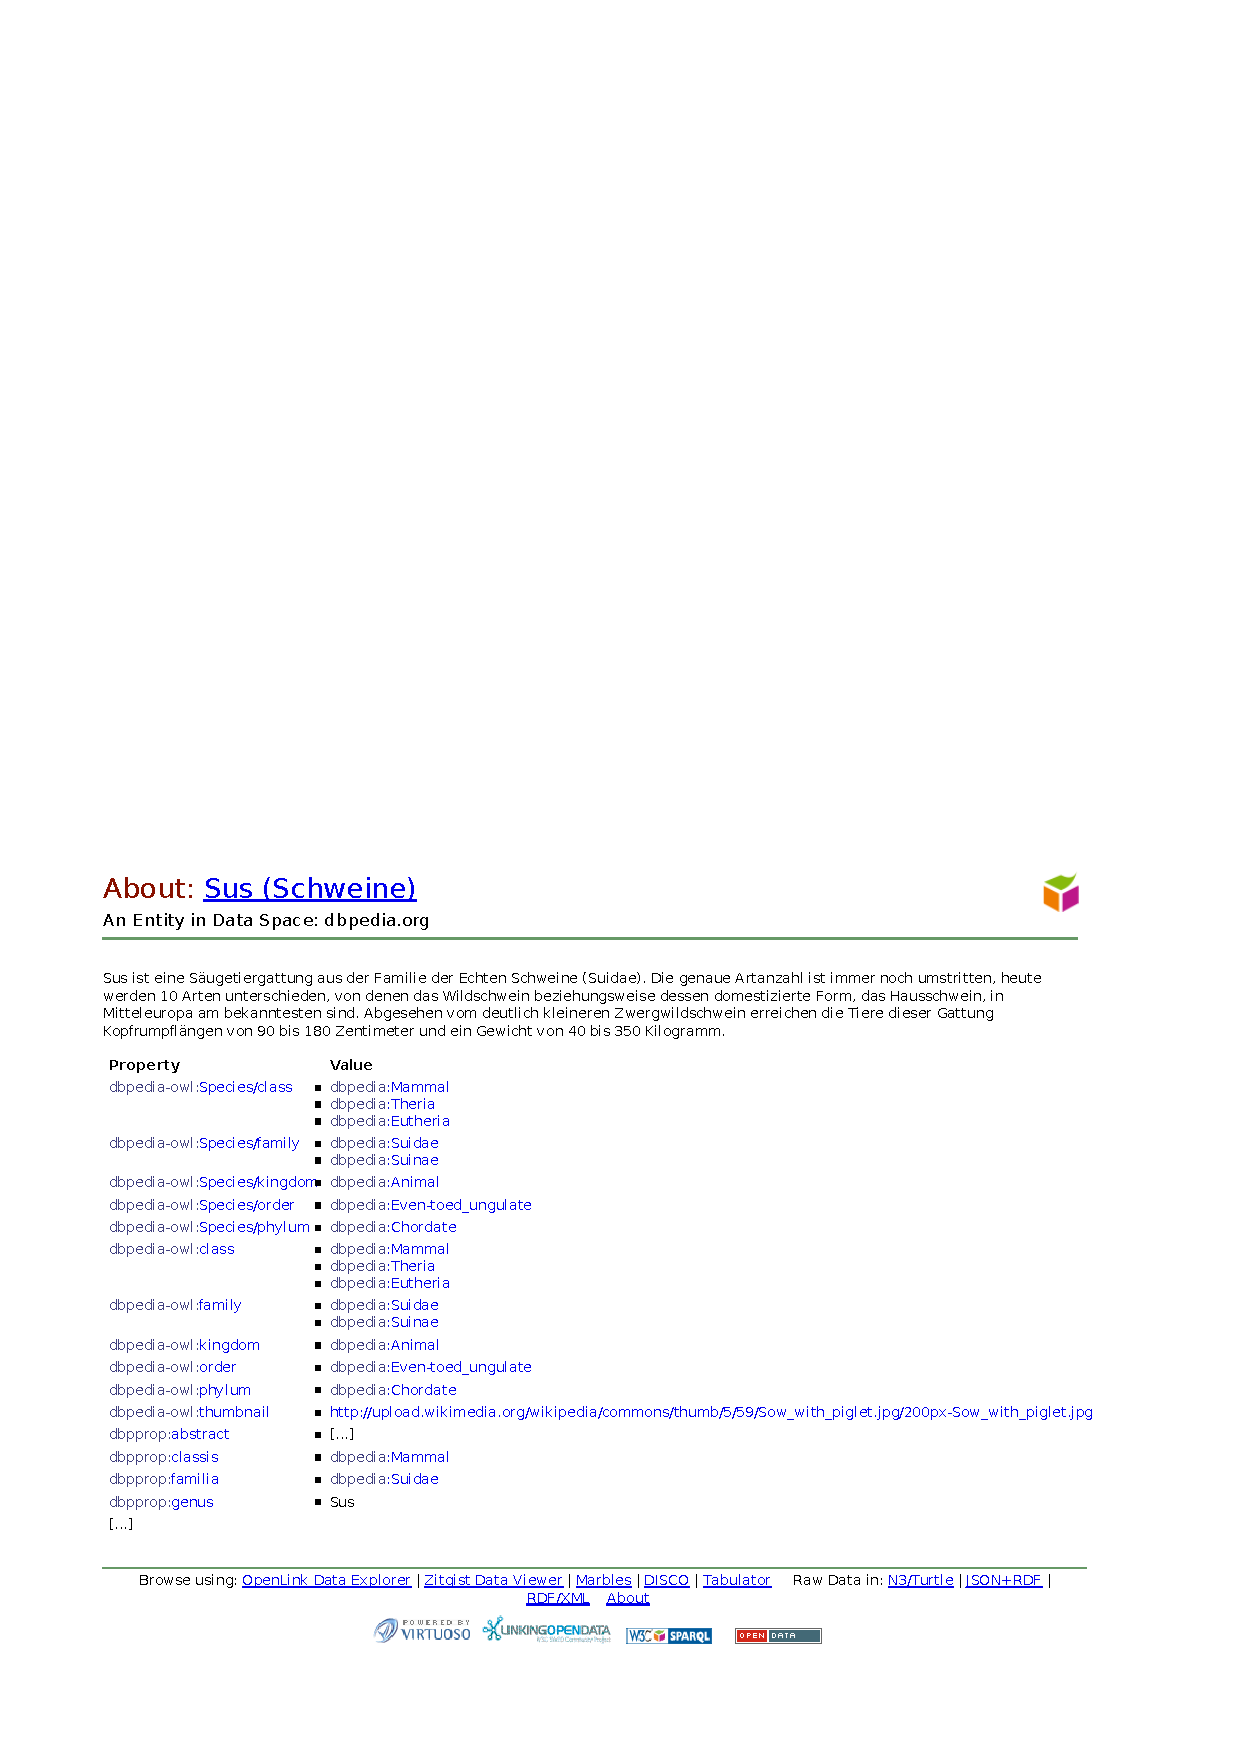
\includegraphics[width=1\textwidth]{img/pdf/pig_anfang.pdf}
\caption[]{Die HTML-Sicht auf den DBpedia-Artikel \url{http://dbpedia.org/resource/pig} (gekürzt, abgerufen am 15.03.2010)}
\label{fig:dbpedia-pig}
\end{figure}

Analog zu \ref{tab:aehnlichkeitsmass-abstracts}:
%Seien $a_1$ und $a_2$ die zu vergleichenden Artikel. 
Seien $P_1$ und $P_2$ die Mengen der enthaltenen Properties sowie v$_1(w)$ und v$_2(w)$ die Anzahl der Vorkommen von $p$ in den beiden DBpedia-Artikeln und f$(p)$ die "`Frequenzklasse"'\footnotemark{} von $p$.
\footnotetext{Analog zur Frequenzklasse von Wörtern: Sei $\f'(p)$ die Frequenz einer Property (die Anzahl der Ressourcen der DBpedia, die mindestens eine Property vom Typ $p$ haben)  und $\f'_{\max}$ die Frequenz der häufigsten Property.
Dann gilt für die Frequenzklasse f der Property:
$f(p)=_{\textnormal{def}}\func{log}_2 \frac{\f'_{\max}}{\f'(p)}$. Bei der Berechnung der Frequenzklasse der Properties wurde auf das Runden verzichtet (im Gegensatz zu der Frequenzklasse der Wörter), es handelt sich also um Fließkommazahlen.}
Da, wie an den Abbildungen \ref{fig:powerlaw_properties_logarithmic_scale} und \ref{fig:zipf_wortschatz_properties} erkennbar ist, auch die Properties $p$ der Entitäten Zipfs Gesetz folgen,
lassen sich auch diese in Frequenzklassen $\f(p)$ einteilen und es ist möglich, eine der im vorigen Kapitel gewählten Gewichtung Ähnliche anzuwenden.
Dann ergibt sich:
%Weiterhin $s_{\max}$ die maximale mögliche Anzahl an Übereinstimmungen der beiden Abstracts sowie $\s_\textnormal{abs}$
%Sei nun s die Funktion s$_{\max}$\\
\begin{subequations}
\begin{align}
\s&_{\textnormal{abs}} 	&:=& \sum_{p\in P_1\cap P_2} \f(p)\cdot\sqrt{\func{v}_1(p)\cdot	\func{v}_2(p)}\\
\s&_{\max}		&:=& \sum_{p\in P_1\cup P_2} \f(p)\cdot\frac{\func{v}_1(p)+	\func{v}_2(p)}{2}\\
\s_{p_1}	&		&:=& \frac{\s_{\textnormal{abs}}}{\s_{\max}}
\end{align}
\label{tab:aehnlichkeitsmass-semantisch}
\end{subequations}

% \subsubsection{Verteilung der Properties}\label{sec:verteilung}
% Um die Gewichtung einer Property, also ihren angenommenen Informationsgehalt, für das semantische Ähnlichkeitsmaß festzulegen, wurde die Verteilung der Properties anhand ihrer Vorkommenshäufigkeit betrachtet.
% Dabei wurde eine Verteilung gemäß eines \emph{power laws}, also eines Potenzgesetzes festgestellt.
% \paragraph{Potenzgesetze}
% Potenzgesetze (engl. \emph{power laws}) beschreiben in der Statistik eine bestimmte Art mathematischer Beziehung zweier Größen und haben die Form
% $f(x) = y = a \cdot x^k+o(x^k)$. Dabei sind $a$ und $k$ Konstanten und $o(x^k)$ ist gegenüber $x^k$ asymptotisch vernachlässigbar.
% Die Funktion f ist \emph{skaleninvariant} mit Skalierungsexponent $k$, das heißt $f(x) \propto f(c\cdot x)$ für jedes $c \in \setR$.
% Aufgrund der teilweise sehr extremen Verteilungen ist es oft schwer, eine solche Beziehung als einem Potenzgesetz entsprechend einzustufen (siehe Abbildung \ref{fig:powerlaw_properties_linear_scale}).
% \begin{figure}[tbh]
% \includegraphics[width=\textwidth]{img/pdf/powerlaw_properties_linscale.pdf}
% \caption[]{Verteilung der Properties der DBpedia bezüglich ihrer Nutzungshäufigkeit (linearer Maßstab)}
% \label{fig:powerlaw_properties_linear_scale}
% \end{figure}
% Aus $y = a \cdot x^k$ folgt $\log(y)= \log(a) + k \cdot \log(x)$.
% Auf einer Darstellung mit logarithmischen Achsen lässt sich also ein linearer Zusammenhang erkennen, falls eine Verteilung gemäß einem Potenzgesetz besteht (siehe Abbildung \ref{fig:powerlaw_properties_logarithmic_scale}).
\begin{figure}[tbh]
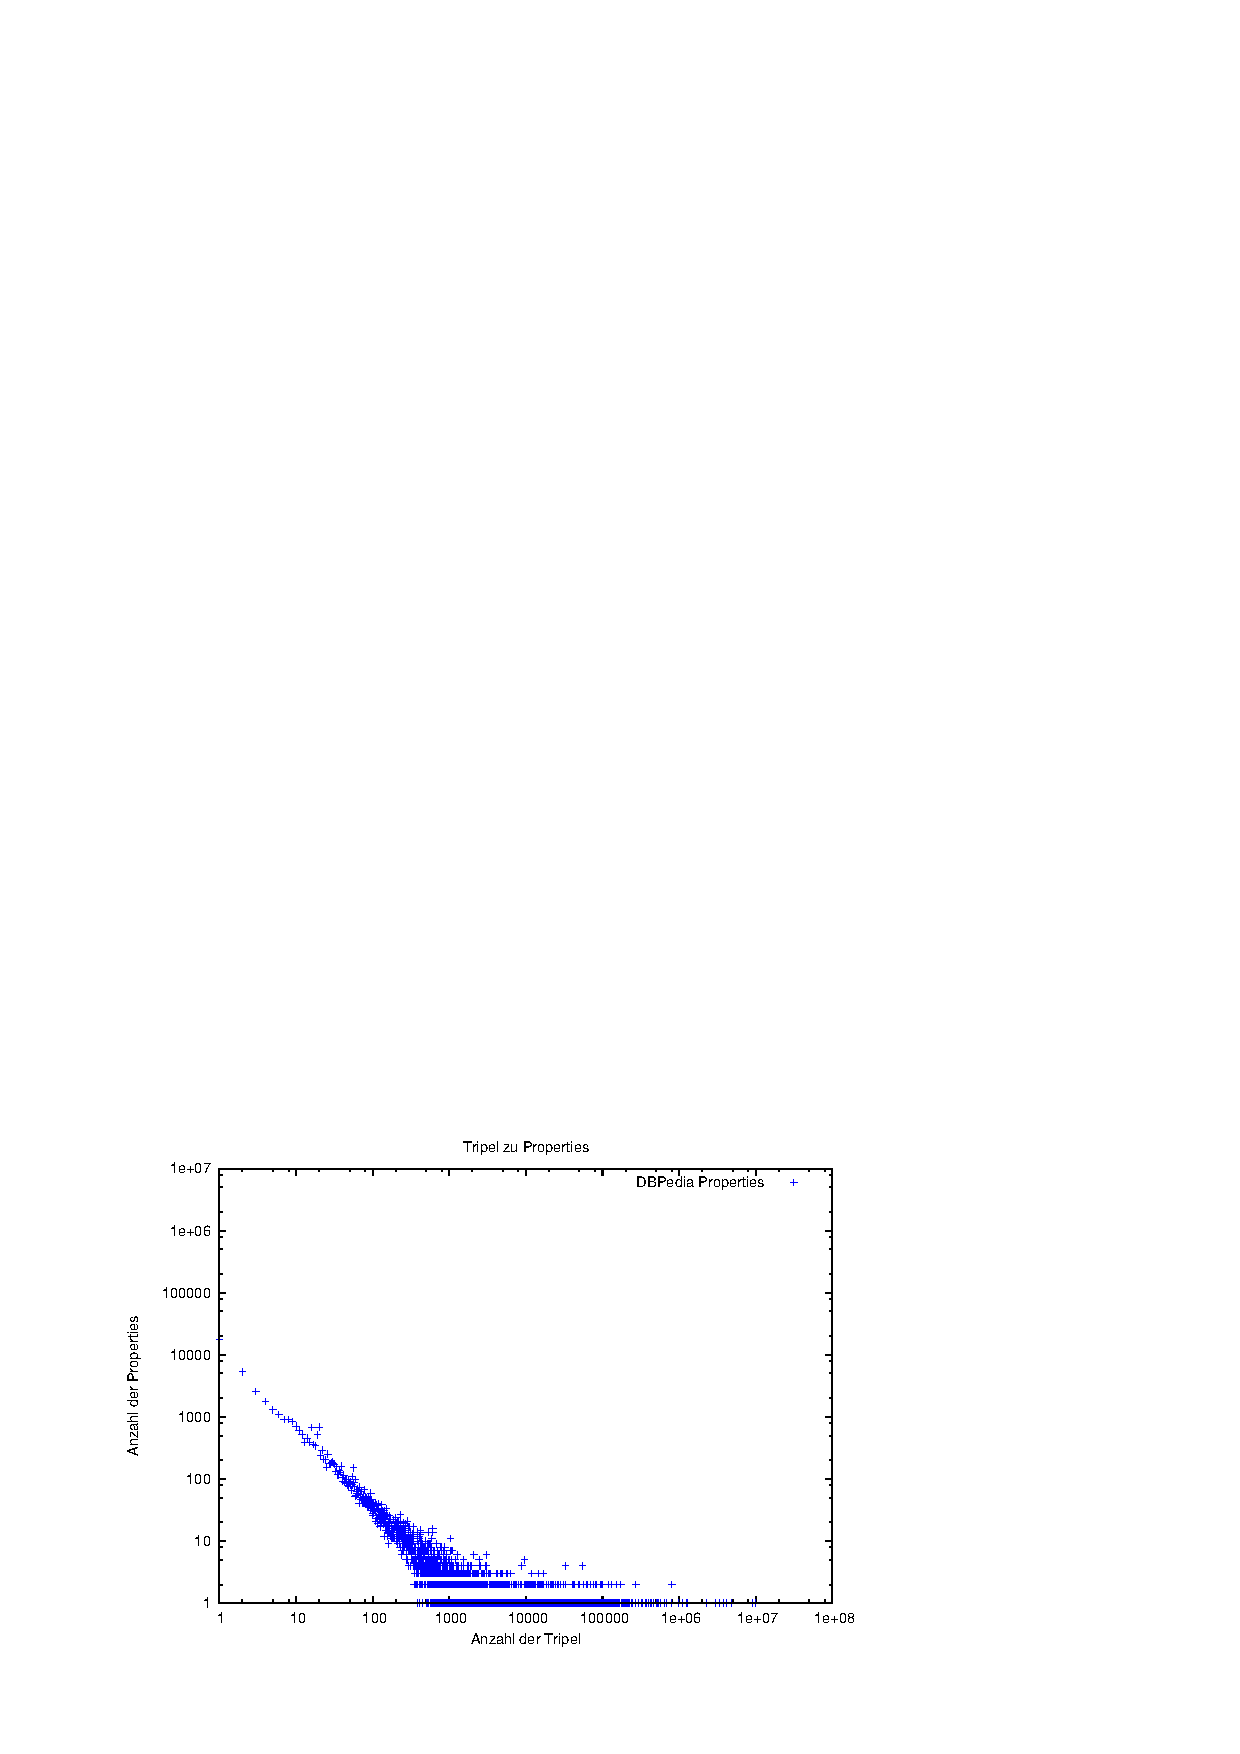
\includegraphics[width=\textwidth]{img/pdf/powerlaw_properties.pdf}
\caption[]{Verteilung der Properties der DBpedia bezüglich ihrer Nutzungshäufigkeit (logarithmischer Maßstab)}
\label{fig:powerlaw_properties_logarithmic_scale}
\end{figure}
%Sehr viele natürliche Phänomene lassen sich mit Potenzgesetzen beschreiben, \zb{} die Größe von Städten, 
% \begin{figure}[tbh]
% 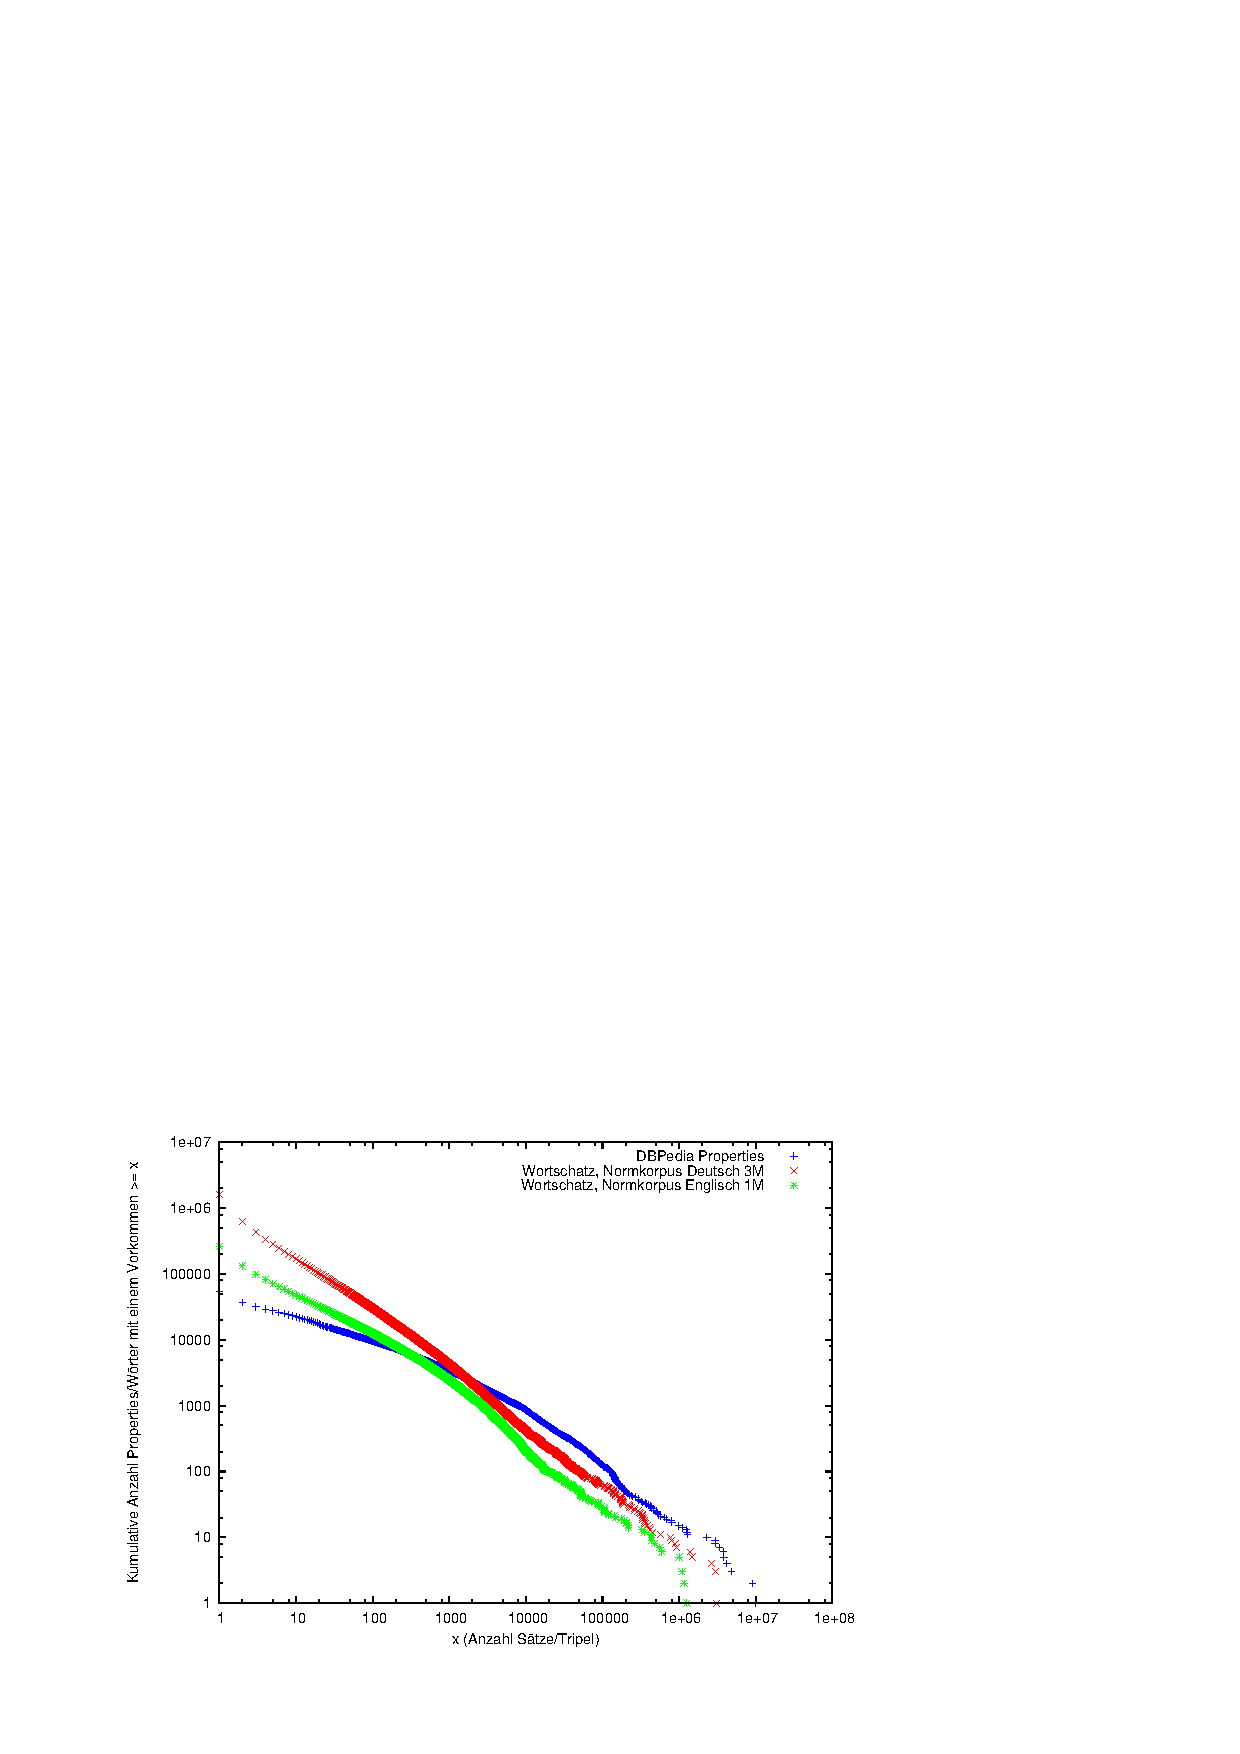
\includegraphics[width=\textwidth]{img/pdf/pareto_wortschatz_properties.pdf}
% %\caption{}
% \label{fig:pareto_wortschatz_properties}
% \end{figure}

\begin{figure}[tbh]
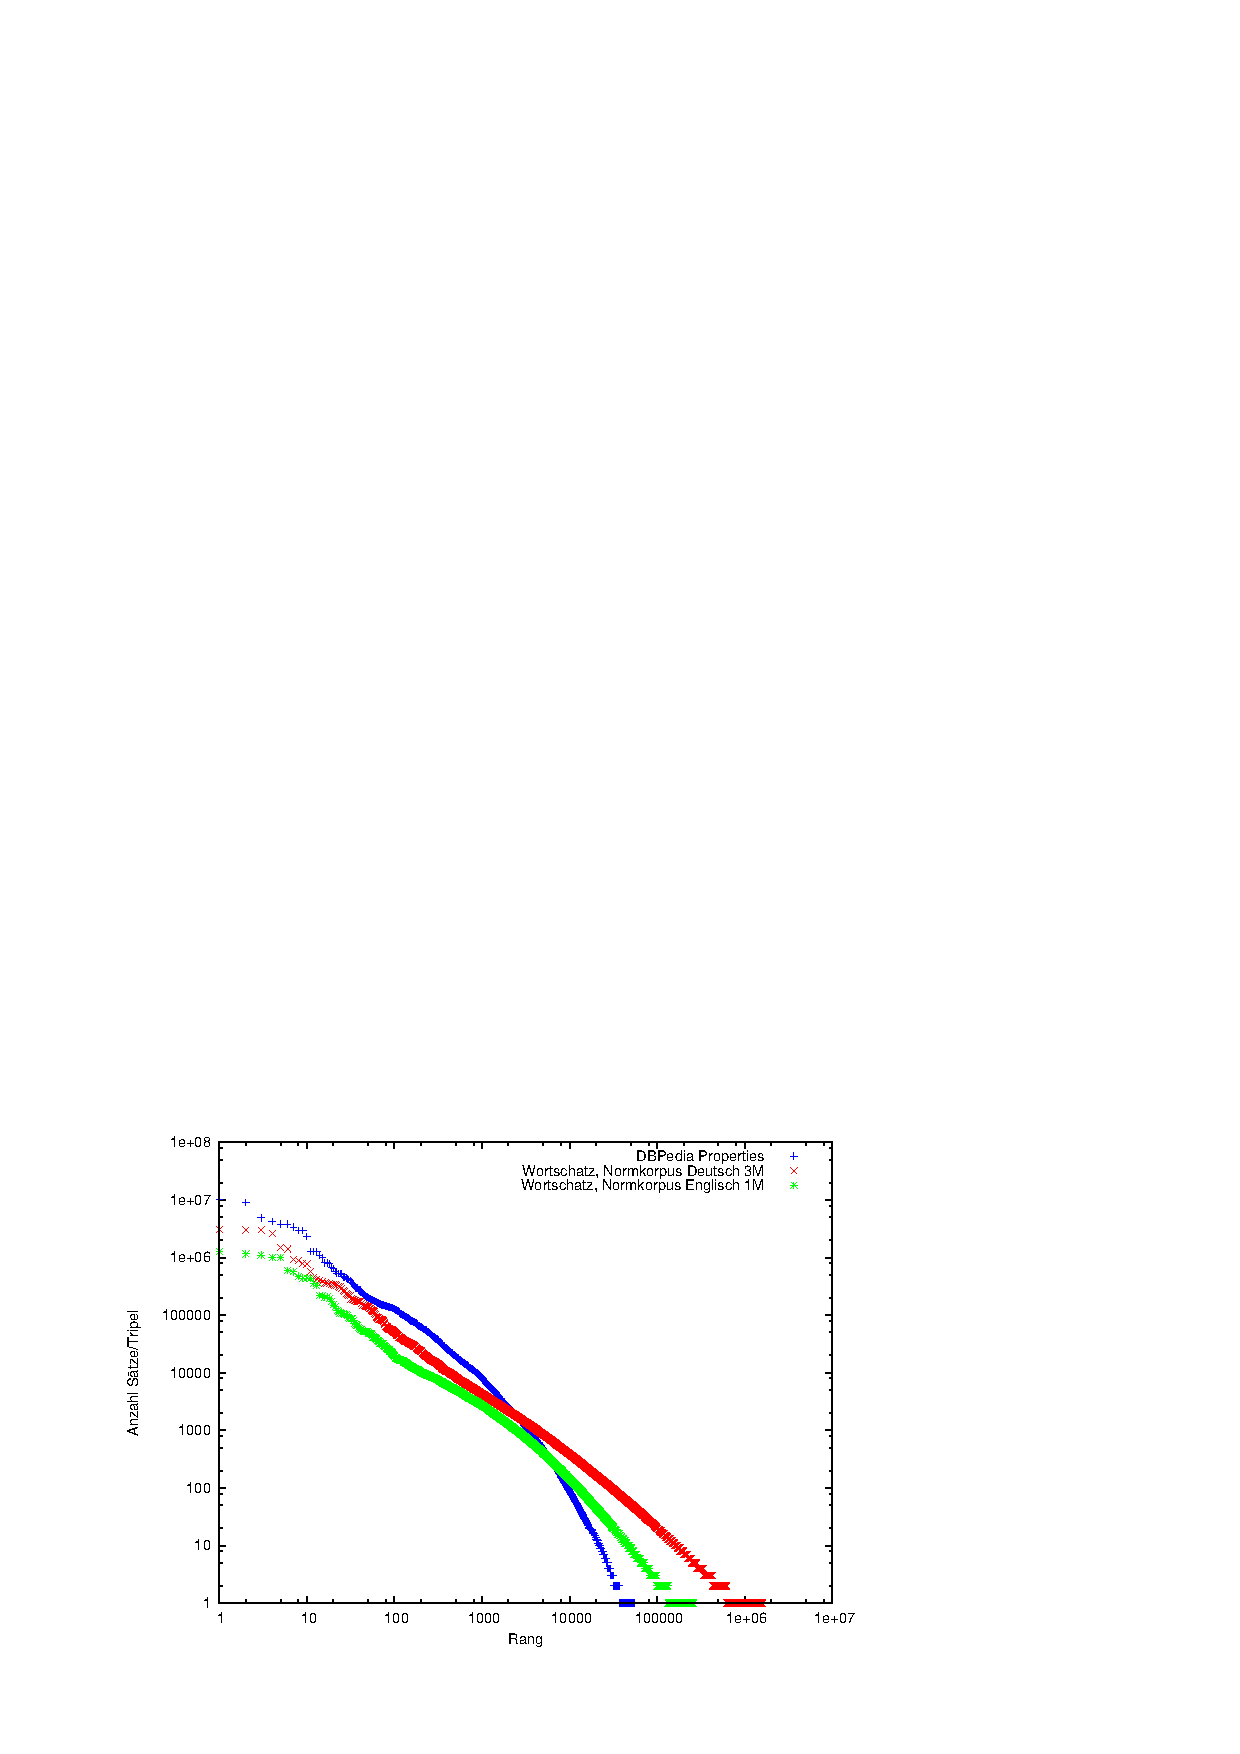
\includegraphics[width=\textwidth]{img/pdf/zipf_wortschatz_properties_reduced.pdf}
%\caption{}
\label{fig:zipf_wortschatz_properties}
\end{figure}

% \begin{figure}[tbh]
% 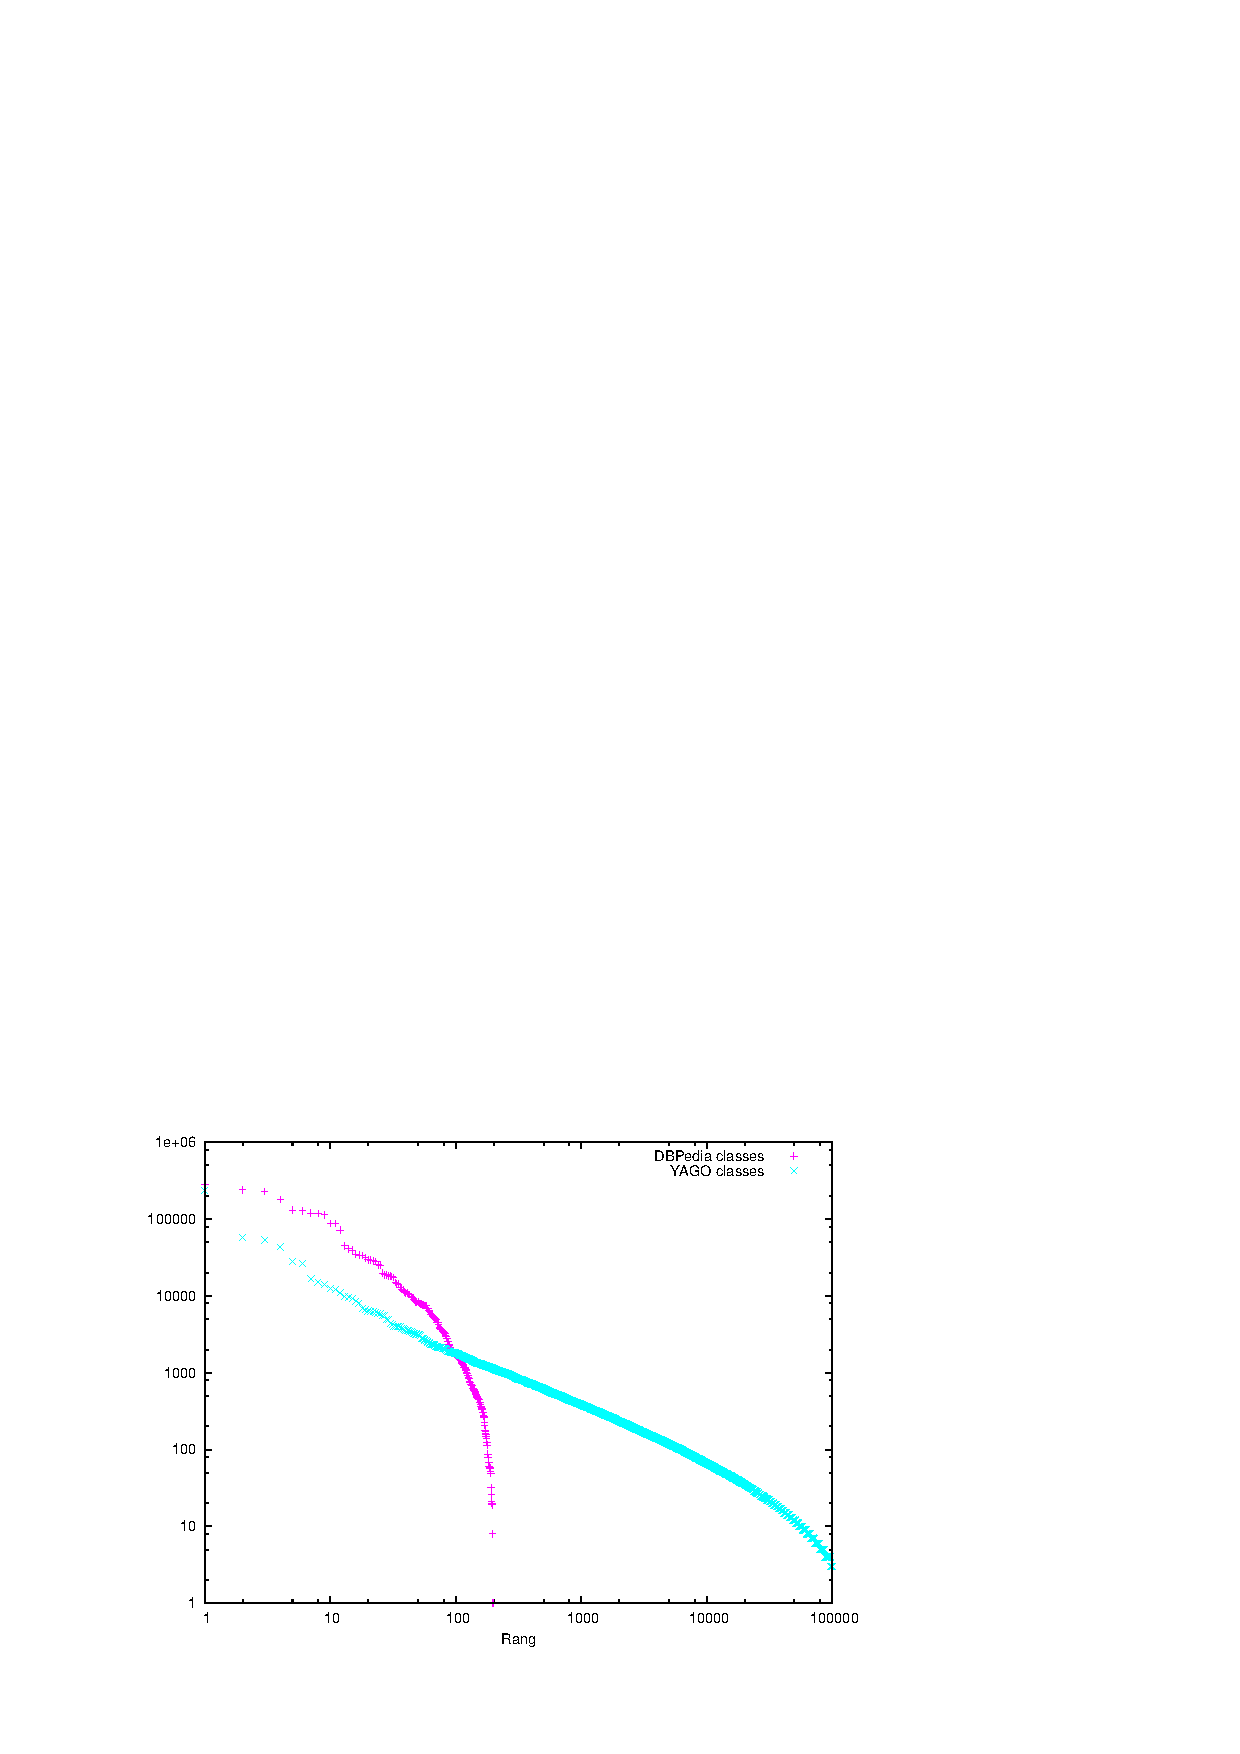
\includegraphics[width=\textwidth]{img/pdf/zipf_hierarchy_reduced.pdf}
% %\caption{}
% \label{fig:zipf_hierarchy}
% \end{figure}

%Außerdem wird die Nähe der zu vergleichenden Klassen in verschiedenen Hierarchien als Hinweis auf eine Ähnlichkeit gewertet.

%umgedreht könnte man auch machen wird aber nicht gemacht

Ein wichtiger Unterschied zwischen den Abstracts der Wikipedia-Artikel und der aus diesen Artikeln extrahierten DBpedia-Daten ist jedoch, dass
die Einleitungen alle ungefähr die gleiche Länge haben und von Menschen mit dem Zweck geschrieben wurden, alle relevanten Informationen zu diesem Thema aufzuführen.
Aus diesem Grund kann das Vorkommen eines Wortes in dem einen Abstract und das Fehlen desselben im Anderen als Indiz dafür aufgefasst werden, dass das eine Konzept ein bestimmtes Merkmal aufweist,
das Andere jedoch nicht. Weiterhin kann die Anzahl der Vorkommen des Wortes Hinweise auf auf die Stärke der Ausprägung des Merkmals geben.
Da die Länge der Wikipedia-Artikel jedoch stark variiert und die Properties nur aus einem Teil der Artikel gewonnen werden (vor allem aus den Infoboxen), ist es fraglich, ob die Anzahl des Vorkommens
einer bestimmten Property in den Ähnlichkeitswert einfließen sollte oder ob die wichtigste Information ist, dass beide Konzepte überhaupt diese Property aufweisen.

\begin{bsp}
Wir vergleichen die Artikel \article{Gordon_Bethune} und \article{Sam_Walton}.
Beide weisen die Property \property{dbpedia-owl:occupation} auf.\\
~\\
\article{Gordon_Bethune} \property{dbpedia-owl:occupation}
\begin{itemize}
\item \article{dbpedia:Continental_Airlines}
\item \article{dbpedia:Braniff}
\item \article{dbpedia:Boeing}
\item \article{dbpedia:Piedmont_Airlines}
\end{itemize}
\article{Sam_Walton} \property{dbpedia-owl:occupation}
\begin{itemize}
\item \article{dbpedia:Wal-Mart}
\item \article{dbpedia:Chairman}
\end{itemize}
\end{bsp}

Die wichtige Information hierbei ist, dass beide Entitäten eine Arbeit besitzen oder besaßen, also Arbeiter sind oder waren.
Dass die eine Person dabei bereits vier Stellen besaß und die andere Zwei (tatsächlich wohl nur eine, da \emph{Chairman} sicherlich eine Position ist und kein Arbeitgeber), ist in diesem Fall kein wesentliches Merkmal.
Aufgrund der \emph{Open World Assumption} kann es ja weitere Angestelltenbeziehungen geben, die nur nicht in der DBpedia enthalten sind.
Aus diesem Grund wurde die Vorkommenshäufigkeit v$(p)$ aus Formel \ref{tab:aehnlichkeitsmass-semantisch} entfernt.
%Es ist also fraglich, ob die Vorkommenshäufigkeit v$(p)$ in Formel \ref{aehnlichkeitsmass-semantisch} zu integrieren ist oder nicht.
%Da es jedoch unklar ist, inwieweit dieses Beispiel zu verallgemeinern ist, wurden beide Möglichkeiten implementiert und in die Evaluierung der Disambiguierung einbezogen.
Natürlich ist nicht nur das gemeinsame Vorhandensein einer Property (\emph{schwache Beziehung} in Tabelle \ref{tab:beispiel-aehnlichkeitsmass}) eine wichtige Information sondern auch, worauf sie verweist.
Sind die Objekte bei beiden Artikeln dieselben (\emph{indirekte Beziehung} in Tabelle \ref{tab:beispiel-aehnlichkeitsmass}), ist dies natürlich ein stärkerer Indikator für eine Übereinstimmung.
%Ist dies nicht der Fall, kann die Ähnlichkeit dieser Objekte noch rekursiv mittels t oder auch mittels eines taxonomischen Vergleiches berechnet werden, dies wurde jedoch aus Laufzeitgründen nicht durchgeführt.
Aus diesen Überlegungen ergibt sich:

\begin{subequations}%\label{aehnlichkeitsmass-semantisch}
\begin{align}
\func{s}&_{\textnormal{abs}} 	&:=& \sum_{p\in P_1\cap P_2} \f(p)\cdot \alpha \\
\func{s}&_{\max}		&:=& \sum_{p\in P_1\cup P_2} \f(p)
\end{align}
\end{subequations}

Mit
$\alpha = 
\begin{cases}
1 &\exists o: (a_1,p,o) \land (a_2,p,o)\footnotemark{}\\%\textnormal{{falls beide Artikel ein Vorkommen von $p$ mit demselben Objekt o haben}\\
c &\textnormal{sonst}, 0 < c < 1
\end{cases}$
\footnotetext{Informell: Falls beide Artikel ein Vorkommen der Property $p$ mit demselben Objekt $o$ haben.}

Daraus ergeben sich jedoch Schwierigkeiten:
Ist $c$ zu klein, dann wird die Bedeutung des Vorhandenseins gleicher Properties unterschätzt, ist $c$ zu groß, dann wird sie überschätzt und das alleinige Vorhandensein einer seltenen Property 
kann schwerer wiegen als die Übereinstimmung in einer häufigen Property inklusive desselben Objektes. Sehr häufige Properties wie \property{rdf:type} oder \property{skos:subject} fallen sogar ganz weg,
da sie eine Frequenzklasse von 0 besitzen. Außerdem sind durch die Multiplikation mit $c$ die resultierenden Ähnlichkeitswerte sehr klein.
Dieses Problem wird behoben, indem die Frequenzklasse nicht einbezogen wird, falls Objektgleichheit vorliegt:

\begin{equation}
\s_{\textnormal{abs}} := \sum_{p\in P_1\cap P_2}
\begin{cases}
d &\exists o: (a_1,p,o) \land (a_2,p,o), d > 1\\
\f(p) &\textnormal{sonst}\\%\textnormal{{falls beide Artikel ein Vorkommen von $p$ mit demselben Objekt o haben}\\
\end{cases}
\end{equation}

Um die Normierung zu gewährleisten folgt daraus:
\begin{equation}
\s_{\max} := \sum_{p\in P_1\cup P_2} \max(\f(p),d)\\
\end{equation}

\begin{rem}\label{rem:properties-exclusion-1}
Einige der häufigsten Properties werden nicht in die Berechnung einbezogen.
\begin{figure}[H]
\property{rdf:type}\\
\property{skos:subject}
%\end{quote}
\caption{Properties, die Klassenzugehörigkeiten anzeigen}
\label{fig:properties_exclusion_1}
\end{figure}
Diese Properties werden separat über Hierarchien behandelt, siehe Abschnitt \ref{sec:hierarchien}.
Weitere Properties wurden ausgeschlossen, weil sie Artikeldetails beschreiben, die keine Hinweise auf die Ähnlichkeit der beschriebenen Gegenstände liefern, siehe Abbildung \ref{fig:properties_exclusion_2}.
\begin{figure}[H]
%\begin{quote}
\property{dbpprop:wikiPageUsesTemplate}\\
\property{dbpprop:imageWidth}\\
\property{foaf:depiction}\\
\property{foaf:name}\\
\property{foaf:page}\\
\property{dbpprop:imageCaption}\\
%\end{quote}
\caption{ausgeschlossene Properties}
\label{fig:properties_exclusion_2}
\end{figure}
\end{rem}

Bei einer ersten Auswertung des Ähnlichkeitsmaßes $s_p$ angewandt auf die Testdaten aus Abschnitt \ref{sec:aehnlichkeitsmass-abstract} (siehe Tabelle \ref{tab:aehnlichkeitsmass-semantisch-properties-1})
ergibt sich ein sehr hoher Wert für das Paar (\article{Wild_boar}, \article{Pig}).
Nimmt man die gleiche Einteilung vor wie bei Tabelle \ref{tab:einschaetzung}, dann ergibt sich folgende Reihenfolge:
\begin{center}
\begin{tabular}{lllllll}
1	&$>$	&$3,9$	&$>$	&$6, 10, 2, 8$	&$>$ &$5,7,4$\\
\end{tabular}
\end{center}
Dieses Ergebnis stimmt nicht mit der manuellen Einschätzung aus Tabelle \ref{tab:einschaetzung} überein.
Weiterhin fällt auf, dass in Tabelle \ref{tab:aehnlichkeitsmass-semantisch-properties-1} mehrere Artikelpaare den gleichen Ähnlichkeitswert aufweisen.
Um die Ursache für diese Probleme zu untersuchen, werden die gemeinsamen Properties der getesteten Artikel betrachtet (siehe Tabelle \ref{tab:properties-intersection}).
Unter diesen befinden sich immer noch einige Properties, die Details des Artikels und nicht des Artikelgegenstandes beschreiben.
Abbildung \ref{tab:properties_exclusion_3} zeigt weitere Properties, die daher zusätzlich zu denen aus Abbildung \ref{fig:properties_exclusion_2} entfernt wurden.
\begin{figure}[H]
%\begin{quote}
\property{dbpedia-owl:thumbnail}\\
\property{dbpprop:relatedInstance}\\
\property{dbpprop:wikiPageUsesTemplate}\\
\property{dbpedia-owl:thumbnail}\\
\property{dbpprop:hasPhotoCollection}\\
\property{dbpprop:name}\\
%\end{quote}
\caption{weitere ausgeschlossene Properties}
\label{tab:properties_exclusion_3}
\end{figure}

Eine Anwendung der Ähnlichkeitsmaßes $\s_p$ auf die Testdaten, bei denen auch die Properties aus Tabelle \label{tab:properties_exclusion_3} ignoriert werden, erhöht den Ähnlichkeitswert des Paares (\article{Wild_boar}, \article{Pig}) auf \val{0.9568}, resultiert jedoch
in einem Ähnlichkeitswert von 0 für alle weiteren Paare (siehe Tabelle \ref{tab:aehnlichkeitsmass-semantisch-properties-2}).

Dies liegt daran, dass für alle hier getesteten DBpedia-Artikel bis auf \article{Wild_boar} und \article{Pig} keine ausführlichen Daten vorliegen.
Die Daten der DBpedia werden per automatischer Extraktion aus Wikipedia-Infoboxen erzeugt.
Dadurch kann beispielsweise zwischen den Artikeln \article{Wild_boar} und \article{Elephant} keine Ähnlichkeit festgestellt werden (siehe Abbildungen \ref{fig:wikipedia-wild_boar} und \ref{fig:wikipedia-elephant}).

%foaf:depiction, relatedInstance	&thumbnail, wikiPageUsesTemplate, piction, hasPhotoCollection	&	&~\\
%\midrule
%Starship\_Enterprise	&wikiPageUsesTemplate, name, relatedInstance	&wikiPageUsesTemplate, name, hasPhotoCollection	&wikiPageUsesTemplate, hasPhotoCollection, relatedInstance
%\item [1] Differenzen von weniger als 0,01 wurden als $\approx$ gewertet.

\begin{center}
\begin{table}
\begin{threeparttable}
\begin{tabular}{llll}
\toprule
Artikel 1 		&Artikel 2 		&Ähnlichkeitswert	&$\delta$\tnote{1}\\
\midrule
Wild\_boar		&Pig		&\val{0.8679}		&\val{0.7112}\\
Wild\_boar		&Elephant		&\val{0.1567}		&\val{0.0000}\\
Wild\_boar		&Outer\_space		&\val{0.1567}		&\val{0.0163}\\
Wild\_boar		&Starship\_Enterprise		&\val{0.1404}		&\val{0.0095}\\
Elephant		&Outer\_space		&\val{0.1309}		&\val{0.0048}\\
Pig			&Elephant		&\val{0.1261}		&\val{0.0000}\\
Pig			&Outer\_space		&\val{0.1261}		&\val{0.0163}\\
Pig			&Starship\_Enterprise		&\val{0.1098}		&\val{0.0000}\\
Elephant		&Starship\_Enterprise		&\val{0.1098}		&\val{0.0000}\\
Starship\_Enterprise	&Outer\_space		&\val{0.1098}		&\\
\midrule
$\average$		&			&	0.2034&\\
\bottomrule
\end{tabular}
\begin{tablenotes}
\item [1] In Zeile i: Die Differenz des Ähnlichkeitswertes zwischen Zeile i und Zeile i+1
\end{tablenotes}
\caption{Werte von $s_p$ unter Ausschluß der Properties aus den Abbildungen \ref{fig:properties_exclusion_1} und \ref{fig:properties_exclusion_2}.}
\label{tab:aehnlichkeitsmass-semantisch-properties-1}
\end{threeparttable}
\end{table}
\end{center}

\begin{center}
\begin{table}
\begin{threeparttable}
\begin{tabular}{llll}
\toprule
Artikel 1 		&Artikel 2 		&Ähnlichkeitswert	&$\delta$\tnote{1}\\
\midrule
Wild\_boar		&Pig		&\val{0.9568}		&\val{0.9568}\\
Wild\_boar		&Elephant		&\val{0.0000}		&\val{0.0000}\\
Wild\_boar		&Starship\_Enterprise		&\val{0.0000}		&\val{0.0000}\\
Wild\_boar		&Outer\_space		&\val{0.0000}		&\val{0.0000}\\
Pig		&Elephant		&\val{0.0000}		&\val{0.0000}\\
Pig		&Starship\_Enterprise		&\val{0.0000}		&\val{0.0000}\\
Pig		&Outer\_space		&\val{0.0000}		&\val{0.0000}\\
Elephant		&Starship\_Enterprise		&\val{0.0000}		&\val{0.0000}\\
Elephant		&Outer\_space		&\val{0.0000}		&\val{0.0000}\\
Starship\_Enterprise	&Outer\_space		&\val{0.0000}		&\\
\midrule
$\average$		&			&0.0957		&\\
\bottomrule
\end{tabular}
\begin{tablenotes}
\item [1] In Zeile i: Die Differenz des Ähnlichkeitswertes zwischen Zeile i und Zeile i+1
\end{tablenotes}
\caption{Werte von $s_p$ unter Ausschluß der Properties aus den Abbildungen \ref{fig:properties_exclusion_1}, \ref{fig:properties_exclusion_2} und \ref{fig:properties_exclusion_3}.}
\label{tab:aehnlichkeitsmass-semantisch-properties-2}
\end{threeparttable}
\end{table}
\end{center}


\begin{sidewaystable}
\footnotesize
\begin{tabular}{lp{4cm}p{4cm}p{4cm}p{4cm}}
\toprule
~	&Wild\_boar	&Pig	&Elephant	&Starship\_Enterprise\\
\midrule
Pig	&Species/class, Species/family, Species/kingdom, Species/order, Species/phylum, dbpedia-owl:class, dbpedia-owl:family, dbpedia-owl:kingdom, dbpedia-owl:order, dbpedia-owl:phylum, thumbnail, dbpprop:classis, dbpprop:familia, dbpprop:genus, dbpprop:name, dbpprop:ordo, dbpprop:phylum, dbpprop:regnum, , foaf:name	&	&	&\\
\midrule
Elephant	&thumbnail, relatedInstance, 	&thumbnail, hasPhotoCollection	&	&\\
\midrule
Starship\_Enterprise	&dbpprop:name, relatedInstance, 	&hasPhotoCollection, dbpprop:name, 	&hasPhotoCollection, relatedInstance, 	&\\
\midrule
Outer\_space	&thumbnail, relatedInstance	&thumbnail, hasPhotoCollection	&thumbnail, hasPhotoCollection, relatedInstance	&hasPhotoCollection, relatedInstance\\
\bottomrule
\end{tabular}
\caption[]{
Gemeinsame Properties der Artikel \article{Wild_boar}, \article{Pig}, \article{Elephant}, \article{Starship_Enterprise}. Ohne die in Bemerkung \ref{rem:properties-exclusion-1} aufgeführten Properties.\\
Aus Platzgründen sind einige Präfixe nicht aufgeführt.
}
\label{tab:properties-intersection}
\end{sidewaystable}

\begin{figure}[tbh]
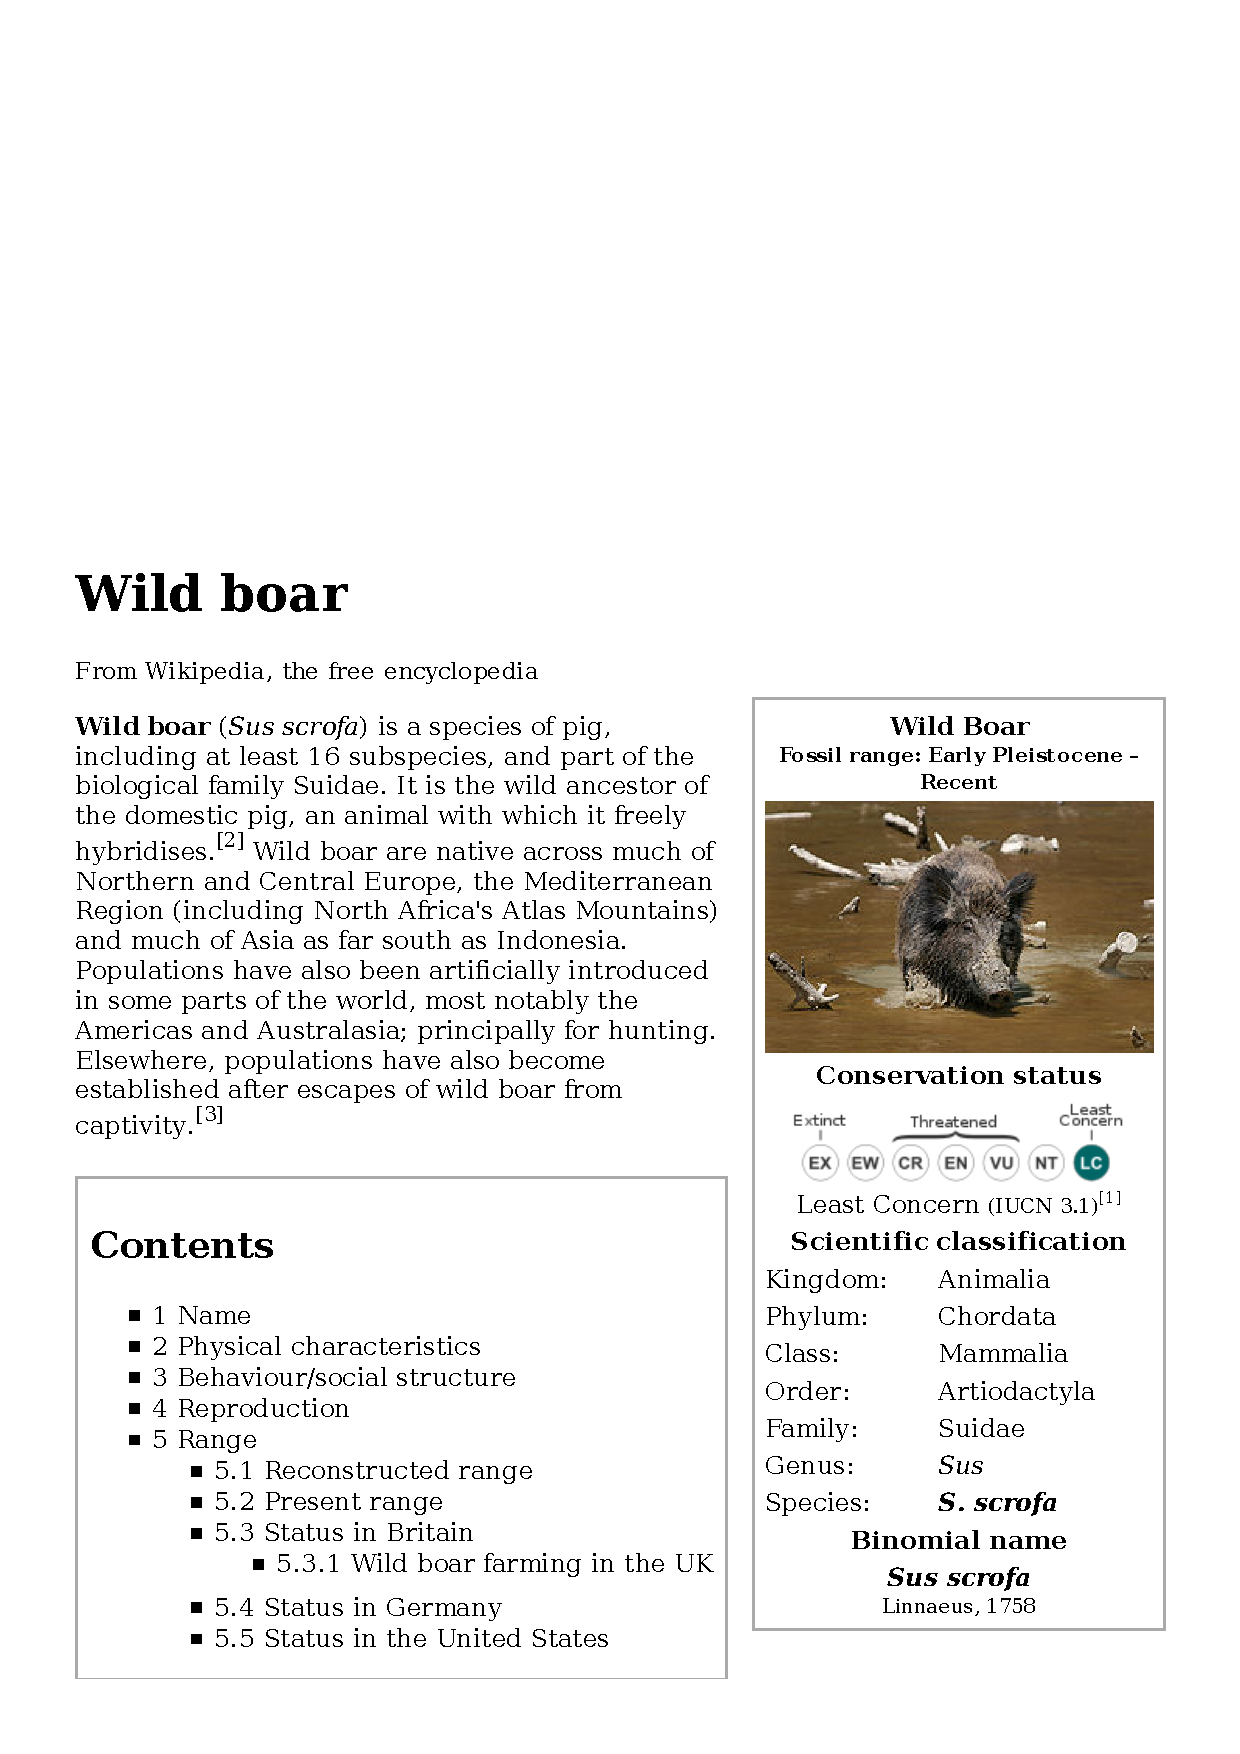
\includegraphics[width=0.99\textwidth]{img/pdf/wild_boar_wikipedia.pdf}
\caption[]{Der Wikipedia-Artikel \url{http://en.wikipedia.org/wiki/Wild_boar} (teilweise abgebildet, aufgerufen am 17.03.2010) enthält eine automatisch verarbeitbare \emph{Infobox}.}
\label{fig:wikipedia-wild_boar}
\end{figure}

\begin{figure}[tbh]
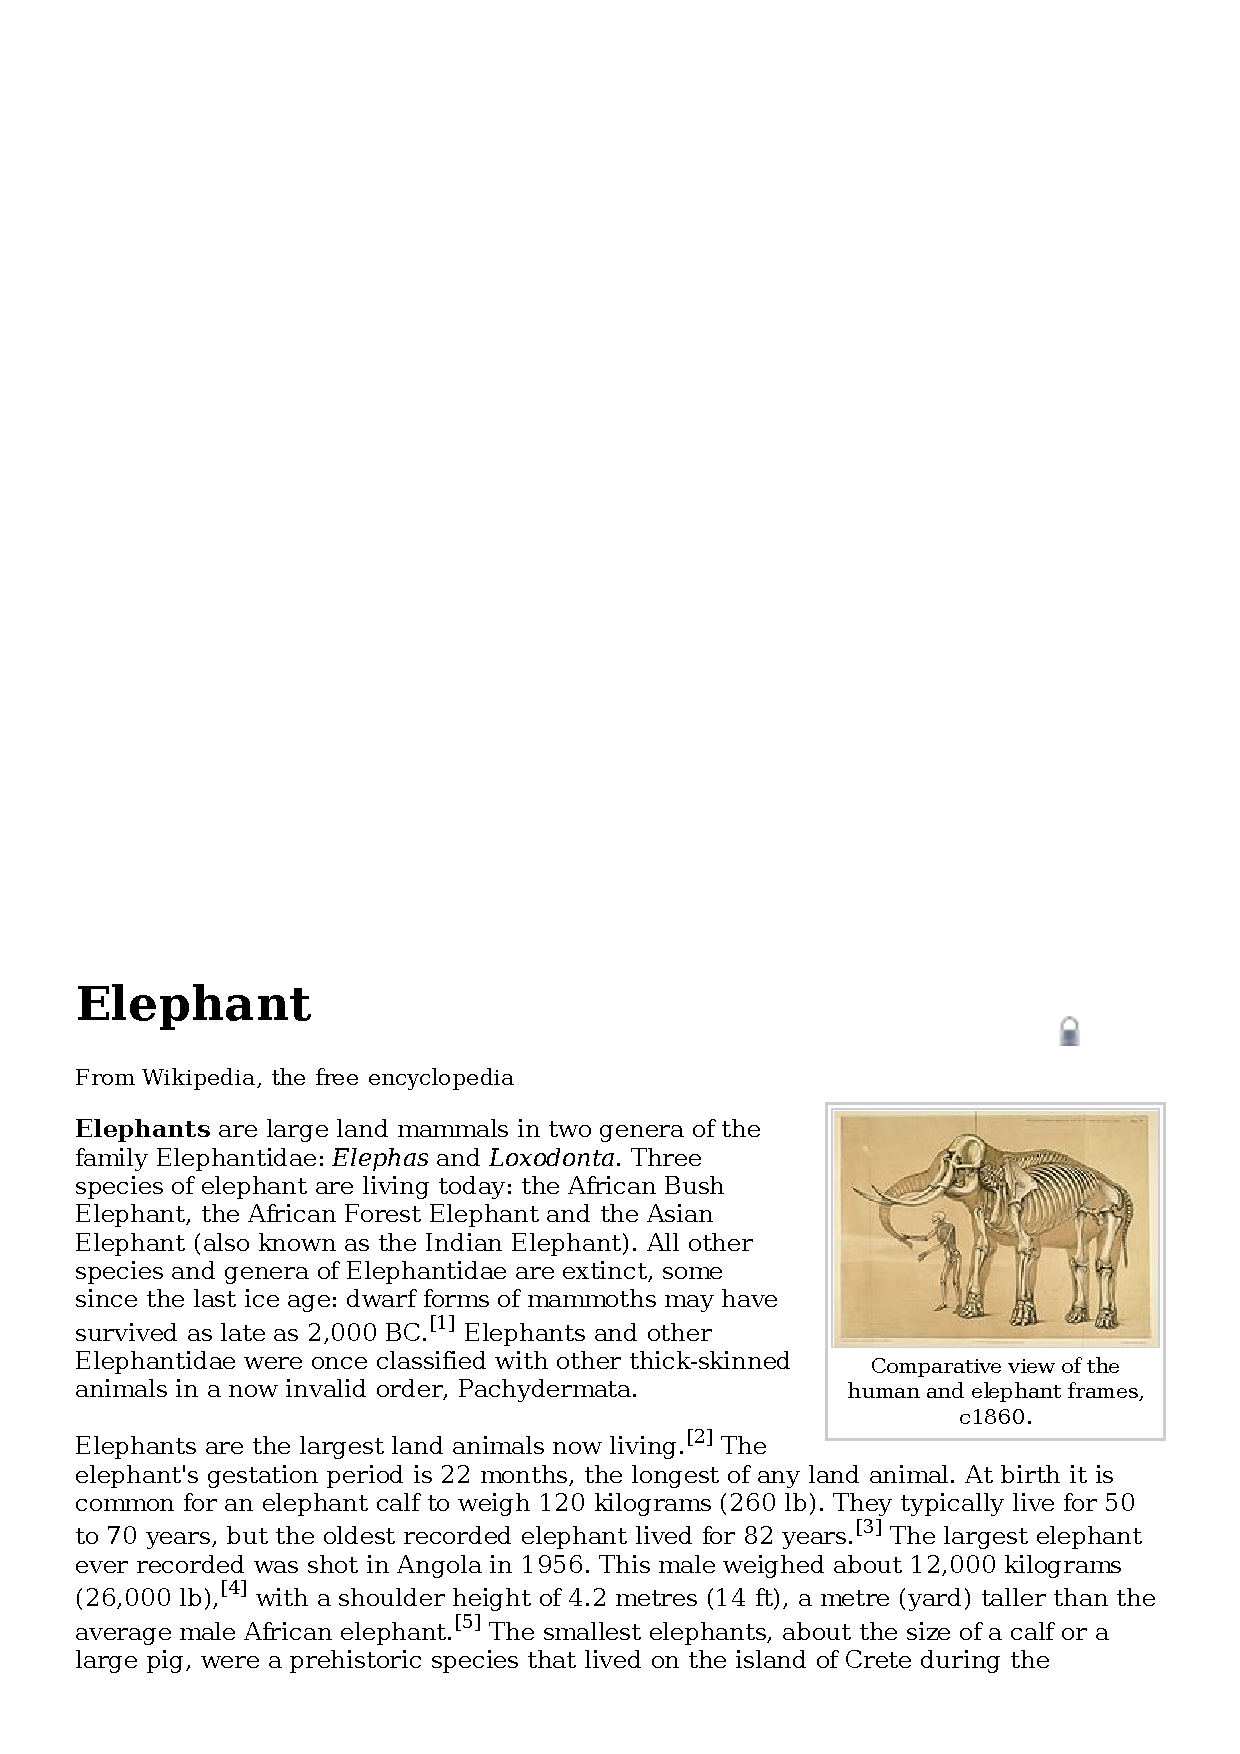
\includegraphics[width=0.99\textwidth]{img/pdf/elephant_wikipedia.pdf}
\caption[]{Der Wikipedia-Artikel \url{http://en.wikipedia.org/wiki/Elephant} (teilweise abgebildet, aufgerufen am 17.03.2010) enthält keine Infobox.}
\label{fig:wikipedia-elephant}
\end{figure}

\subsubsection{Version 2}
Bei näherer Betrachtung von Version 1 des Ähnlichkeitsmaßes der Properties fallen einige Schwächen auf.
So werden Ähnlichkeiten nur dann festgestellt, wenn beide Entitäten dieselbe Property aufweisen und vorzugsweise noch dasselbe Objekt haben.
Es existieren jedoch noch einige weitere Verbindungen, die auf eine Ähnlichkeit oder eine Beziehung zwischen zwei Entitäten schließen lassen.
Aus diesem Grund wurde eine zweite Version des Ähnlichkeitsmaßes entworfen, die eine größere Anzahl an Beziehungstypen in Betracht zieht.
Seien $aRx$ und $bRx$ (bzw. $(a,p,x)$ und $(b,p,x)$) zwei Tripel, wobei $a$ und $b$ als Subject, $R$ bzw. $p$ als property und $x$ als Objekt fungieren.
\begin{table}[h]
\begin{center}
\begin{tabular}{llll}
\toprule
	&Beziehung			&			&Hinweis auf\\
\midrule
a	&direkt				&$aRb \lor  bRa$	&Ähnlichkeit, Beziehungsstärke\\
b	&stark indirekt 		&$aRx \land bRx$	&Ähnlichkeit, Beziehungsstärke\\
c	&schwach indirekt		&$aRx \land bSy$	&Beziehungsstärke\\
d	&gleiche Property		&$aRx \land bRy$	&Ähnlichkeit, Beziehungsstärke\\
\bottomrule
\end{tabular}
\end{center}
\caption{Beziehungstypen zwischen zwei Entitäten $a$ und $b$ in Reihenfolge ihrer Beziehungsstärke}
\label{tab:disambiguierung-properties}
\end{table}

\begin{figure}[H]
\centering
\subfloat[]{
\Tree[2]{
\K{a}\B{d}^{R}\\
\K{b}\\
} 
}
\subfloat[]{
\Tree[-1]
{
		&\K{x}\B{dl}_{R}\B{dr}^{R}\\
\K{a}		&			&\K{b}\\
} 
}
\subfloat[]{
\Tree[-1]
{
		&\K{x}\B{dl}_{R}\B{dr}^{S}\\
\K{a}		&			&\K{b}\\
} 
}
\subfloat[]{
\Tree[-1]
{
\K{a}\B{d}^{R}	&\K{b}\B{d}^{R}\\
\K{x}		&\K{y}\\
} 
}
\end{figure}

Sei $T$ die Menge aller in der DBpedia enthaltenen Tripel und seien $T_a$ und $T_b$ die Mengen der Tripel mit $a$ und $b$ als Subjekt, $T_a = \{t=(s,p,o)\in T| s = a\}$,
$T_b = \{t=(s,p,o)\in T| s = b\}$.
%Seien weiterhin $P_a$ und $P_b$ die Menge aller Properties aus $T_a$ und $T_b$, $P_a = \{p|\exists o: (a,p,o) \in T_a\}$, $P_b = \{p|\exists o: (b,p,o) \in T_b\}$.
Aus Tabelle \ref{tab:disambiguierung-properties} lässt sich nun folgendes Ähnlichkeitsmaß konstruieren:

\begin{align}
\s_{p_2}(a,b)	&= \frac{\sum_{t \in T_a} \s_{p_1}(t,b,T_b)+\sum_{t \in T_b} \s_{p_2}'(t,a,T_a)}{|T_a|+|T_b|}
\end{align}
mit
\begin{equation}
\s_{p_2}'((s,p,o),x,T') = 
\begin{cases}
1 					&\text{wenn } o=x\\
1 					&\text{wenn } \exists (x,p,o) \in T'\\
\alpha<1				&\text{wenn } \exists p': 	\exists (x,p',o) \in T'\\
1-\frac{1}{\val{0.1}\cdot f(p)+1}	&\text{wenn } \exists o':	\exists (x,p,o') \in T'\\
\end{cases} 
\end{equation}
%f(p) die Frequenzklasse der Property ist.
Die einzelnen Fälle lassen sich dabei wie folgt begründen:

\begin{align*}
1 			&\text{  wenn } o=x
\end{align*}
In diesem Fall gilt entweder $t = (a,p,b)$ oder $(b,p,a)$, was eine direkte Beziehung und damit ein starkes Indiz für eine Ähnlichkeit ist.

\begin{align*}
1 			&\text{  wenn } \exists (x,p,o) \in T'\\
\end{align*}
In diesem Fall gibt es eine stark indirekte Beziehung, was auch ein starkes Indiz für eine Ähnlichkeit ist.

\begin{align*}
\alpha<1		&\text{  wenn } \exists p': 	\exists (x,p',o) \in T'\\
\end{align*}
Es existiert eine schwach indirekte Beziehung, was ein etwas schwächeres Indiz für eine Ähnlichkeit ist. Alpha wurde dabei auf $\alpha = 0,7$ festgelegt.

\begin{align*}
1-\frac{1}{0,1 \cdot f(p)+1}	&\text{  wenn } \exists o':	\exists (x,p,o') \in T'\\
\end{align*}

Beide Entitäten haben nur das Vorhandensein der gleichen Property gemein, jedoch mit verschiedenen Objekten. Die Stärke der draus gewonnenen Information ist hierbei davon abhängig, wie häufig die Property $p$ ist.
\article{dbpedia-owl:location} beispielsweise hat ohne gleiches Objekt fast gar keine Aussagekraft, \article{dbpedia-owl:vicePresident} hingegen schon, da es die Aussage erlaubt, dass das Konzept eine Person beschreibt, 
die ein Präsident von etwas ist, was eine starke Einschränkung der Gesamtmenge aller Konzepte ist.
In diesem Fall erfolgt keine Gewichtung verschiedener Terme sondern es ist ein einzelner Ähnlichkeitsteilwert für ein Tripel gesucht. Dieser Wert wurde zunächst durch $1-\frac{1}{f(p)+1}$ (Abbildung \ref{fig:1minus1durch1plusx}) berechnet,
dann jedoch auf $1-\frac{1}{0,1 \cdot f(p)+1}$ (Abbildung \ref{fig:1minus1durch1plusxdurch10}) abgeändert,
um erst ab einer Frequenzklasse von 10 (was einer Property entspricht, die $\approx$ 1000 mal so selten ist wie die Häufigste) einen Wert von 0,5 zu erhalten.

\begin{figure}[H]
\subfloat[$1-\frac{1}{f(p)+1}$]{
\includegraphics[width=0.5\textwidth]{img/pdf/1minus1durch1plusx.pdf}
\label{fig:1minus1durch1plusx}
}
\subfloat[$1-\frac{1}{0,1 \cdot f(p)+1}$]{
\includegraphics[width=0.5\textwidth]{img/pdf/1minus1durch1plusxdurch10.pdf}
\label{fig:1minus1durch1plusxdurch10}
}
\caption{verschiedene Gewichtungen der Frequenzklasse einer Property}
\end{figure}


\subsubsection{Anwendung}
Die Property-basierten Ähnlichkeitsmaße eignen sich gut für Entitäten, die zwar nicht besonders ähnlich sind aber auf gemeinsame Elemente verweisen oder die in den Hierarchien auf der gleichen Stufe stehen.
Die Tabellen \ref{tab:aehnlichkeitsmass-semantisch-properties-version1} und \ref{tab:aehnlichkeitsmass-semantisch-properties-version2} zeigen, dass den Städten aus dem gleichen Land höhere Werte zugewiesen werden.
Da $s_{p_2}$ hier unähnlichere Paare stärker abstraft, wird im Folgenden nur noch $s_{p_2}$ verwendet.

\begin{table}
\begin{tabular}{lll}
\toprule
Konzeptpaar					&Ähnlichkeitswert $\s_{p}$\\
\midrule
Leipzig		&Dresden		&0,5381\\
Borna		&Leipzig		&0,5359\\
London		&Liverpool		&0,4677\\
Borna		&Dresden		&0,4633\\
Dresden		&London		&0,4037\\
Dresden		&Liverpool		&0,4037\\
Leipzig		&London		&0,3359\\
Leipzig		&Liverpool		&0,3359\\
Borna		&London		&0,3322\\
Borna		&Liverpool		&0,3322\\
\bottomrule
\end{tabular}
\caption{Werte der Ähnlichkeitsfunktion $\s_{p}$ von einigen Städten}
\label{tab:aehnlichkeitsmass-semantisch-properties-version1}
\end{table}


\begin{table}
\begin{tabular}{lll}
\toprule
Konzeptpaar					&Ähnlichkeitswert $\s_{p_2}$\\
\midrule
Borna		&Leipzig		&0,4816\\
Leipzig		&Dresden		&0,4094\\
Borna		&Dresden		&0,3863\\
London		&Liverpool		&0,3535\\
Dresden		&London		&0,1652\\
Dresden		&Liverpool		&0,1381\\
Borna		&Liverpool		&0,1185\\
Leipzig		&Liverpool		&0,1062\\
Borna		&London		&0,1021\\
Leipzig		&London		&0,0918\\
\bottomrule
\end{tabular}
\caption{Werte der Ähnlichkeitsfunktion $\s_{p_2}$ von einigen Städten}
\label{tab:aehnlichkeitsmass-semantisch-properties-version2}
\end{table}

\FloatBarrier
\subsection{Ähnlichkeit durch Hierarchien}\label{sec:hierarchien}

Es werden folgende Hierarchien benutzt (näher beschrieben in Abschnitt \ref{sec:grundlagen-hierarchien}):
\begin{itemize}
 \item Wikipediakategorien
 \item YAGO
 \item DBpedia-Klassen
\end{itemize}
\iffalse
@article{DBLP:journals/computer/Brachman83,
  author    = {Ronald J. Brachman},
  title     = {What IS-A Is and Isn't: An Analysis of Taxonomic Links in
               Semantic Networks},
  journal   = {IEEE Computer},
  volume    = {16},
  number    = {10},
  year      = {1983},
  pages     = {30-36},
  bibsource = {DBLP, http://dblp.uni-trier.de}
}

SELECT ?o WHERE
{
<http://dbpedia.org/resource/Ant> a ?o.
}

owl:Thing [http]
<http://sw.opencyc.org/2008/06/10/concept/Mx4rvVjf5JwpEbGdrcN5Y29ycA> [http]
dbpedia:ontology/Species [http]
dbpedia:ontology/Animal [http]
dbpedia:ontology/Insect [http]
dbpedia:ontology/Eukaryote [http]

SELECT ?o WHERE
{
<http://dbpedia.org/resource/Pig> a ?o.
}

owl:Thing [http]
dbpedia:ontology/Species [http]
dbpedia:ontology/Animal [http]
dbpedia:ontology/Mammal [http]
<http://sw.opencyc.org/2008/06/10/concept/Mx4rvVjLLJwpEbGdrcN5Y29ycA> [http]
dbpedia:ontology/Eukaryote [http]

SELECT ?o WHERE
{
<http://dbpedia.org/resource/Pig> skos:subject ?o.
}

:Category:Even-toed_ungulates [http]
:Category:Pigs [http]

PREFIX owl: <http://www.w3.org/2002/07/owl#>
PREFIX xsd: <http://www.w3.org/2001/XMLSchema#>
PREFIX rdfs: <http://www.w3.org/2000/01/rdf-schema#>
PREFIX rdf: <http://www.w3.org/1999/02/22-rdf-syntax-ns#>
PREFIX foaf: <http://xmlns.com/foaf/0.1/>
PREFIX dc: <http://purl.org/dc/elements/1.1/>
PREFIX : <http://dbpedia.org/resource/>
PREFIX dbpedia2: <http://dbpedia.org/property/>
PREFIX dbpedia: <http://dbpedia.org/>
PREFIX skos: <http://www.w3.org/2004/02/skos/core#>

Problem: skos-categorien sind mit skos:broader verbunden statt mit rdf:type
-> egal, wir benutzen sowieso yago
-> mal gucken wies da aussieht
\fi

%Da ein Baum ein Spezialfall eines DAG ist, wird in diesem Abschnitt zuerst eine Methode zur Ähnlichkeitsbestimmung anhand einer Polyhierarchie vorgestellt.
In diesem Abschnitt wird zuerst eine Methode zur Ähnlichkeitsbestimmung anhand einer Polyhierarchie vorgestellt.
Darauf folgt ein laufzeitoptimiertes Verfahren, welches bei Monohierarchien ein exaktes Ergebnis liefert, bei Polyhierarchien jedoch immer noch eine gute Näherung.

% die blätter von dem baum sind dann die instanzen
% und die direkten superklassen sind die typen
% -> nee das ist blöd, die blätter sind die typen und die artikel bilden nen count oder so
% -> obwohl das unintuitiv ist erstes ist vielleicht doch besser
% - in der hierarchie sind aber nur die klassen drin und nicht die instanzen also das 2.
\paragraph{Aufgabenstellung}
Sei $G$ eine Hierarchie, $G = (V,E)$.
Seien $T_1, T_2 \subseteq V$ die Klassen (Typen) der DBpedia-Entitäten $a_1$ und $a_2$. %, $T_{i} = \func{classes}(a_{i})$.
%Sei weiterhin $E^+$ die \emph{transitive Hülle}\footnotemark{} der Relation $E$, sowie $T^\star$ die Menge aller Superklassen von $T$, $T^\star = \{v \in V| \exists t \in T: t E^+ v\}$.
%\footnotetext{$x \ E^{+} \ y : \Leftrightarrow \exists n \geq 0 \ \exists e_1,\dots ,e_n \in V: x \,E \,e_1 \,E \,e_2 \,E \dots \,E \,e_n \,E \,y$.}
Gesucht ist nun ein Ähnlichkeitsmaß $\s_h: \pow{V} \times \pow{V} \rightarrow [0,1] \subset \setR$.

\paragraph{Erster Lösungsansatz}
\newcommand{\snaiv}{\s_{\h_0}}
Ein naiver Ansatz ist, den Anteil gleicher Klassen der beiden Individuen zu bestimmen:
\begin{equation*}
\snaiv := \frac{|(T_1 \cap T_2)|}{|(T_1 \cup T_2)|} 
\end{equation*}

Diese Methode ermöglicht jedoch nur eine sehr mangelhafte Aussage über die Ähnlichkeit der Entitäten $a_1$ und $a_2$.
Klassen, die nicht übereinstimmen, führen zu einer Abwertung des Ähnlichkeitswertes.
Aufgrund der Offene-Welt-Annahme ist jedoch auch bei den Entitäten, deren Zuordnung zu einer bestimmten Klasse nicht explizit definiert wurde, die Zugehörigkeit zu dieser Klasse möglich.
Weiterhin sorgt diese Methode für sehr hohe Ähnlichkeitswerte bei Paaren, die eine sehr geringe Anzahl an Klassenzuordnungen besitzen, welche sehr nahe an der Wurzel liegen.

\begin{table}
\begin{tabular}{ll}
\toprule
Entität		&Klassen\\
\midrule
London		&owl:Thing, City\\
Pig		&owl:Thing, Animal\\
Elephant	&owl:Thing, Animal\\
Dog		&owl:Thing, Animal, Mammal, Carnivora\\
Human		&owl:Thing, Animal, Mammal, Primate\\
Mensch		&owl:Thing, Animal, Mammal, Primate\\
\bottomrule
\end{tabular} 
\caption{fiktive Klassenzuordnung einiger Individuen}
\label{tab:klassenzuordnung_fiktiv}
\end{table}

\begin{table}
\begin{tabular}{ll}
\toprule
Konzeptpaar $p$					&Ähnlichkeitswert $\snaiv(p)$\\
\midrule
$($\article{London}$,$\article{Pig}$)$		&0,5\\
$($\article{Pig}$,$\article{Elephant}$)$ 	&1\\
$($\article{Human}$,$\article{Dog}$)$		&0,8\\
$($\article{Human}$,$\article{Mensch}$)$	&1\\
\bottomrule
\end{tabular}
\caption{Werte der Ähnlichkeitsfunktion $\snaiv$ von einigen Paaren von Entitäten aus Tabelle \ref{tab:klassenzuordnung_fiktiv}}
\label{tab:snaiv_werte}
\end{table}

Obwohl in Tabelle \ref{tab:klassenzuordnung_fiktiv} mehr Hinweise auf eine starke Ähnlichkeit zwischen \article{Human} und \article{Dog} vorliegen, als zwischen \article{Pig} und \article{Elephant},
zeigt Tabelle \ref{tab:snaiv_werte}, dass $\snaiv($\article{Human}$,$\article{Dog}$)$ nur einen Wert von $\frac{3}{5} = \val{0.8}$, $\snaiv($\article{Pig}$,$\article{Elephant}$)$ jedoch einen Wert von 1 annimmt.
\FloatBarrier
\paragraph{Fortgeschrittener Lösungsansatz}
%Dieser Ansatz befasst sich mit der Frage nach der \emph{gewonnenen Information} durch eine Angabe von Klassen.
Dieser Ansatz befasst sich mit der Frage, wie genau eine Menge von Eigenschaften ein Objekt charakterisiert.
Gibt es nur ein einziges Objekt, für das diese Eigenschaften zutreffen, dann ist es mit diesen eindeutig identifizierbar.
Die Eigenschaften \emph{"`schwarz"'} und \emph{"`US-Präsident"'} treffen etwa auf nur eine Person zu (\emph{Barrack Obama}),
die gewonnene Information durch diese Angabe ist also maximal.
Die Eigenschaften \emph{"`grün"'} und \emph{"`Grashalm"'} treffen jedoch auf sehr viele Objekte zu, der Informationsgehalt ist also gering.
Die Ähnlichkeit einer Menge von Objekten wird nun dem Informationsgehalt der gemeinsamen Eigenschaften gleich gesetzt,
\begin{equation*}
\s_\h(M) := \func{I}(\bigcap_{m\in M} m) 
\end{equation*}
%Die durch solch eine Zuordnung gewonnene Information entspricht dem Ausmaß der Einschränkung der Menge der Entitäten.
%Die aus einer Menge von Klassen erhaltene Information ist also umgekehrt proportional zur Anzahl der Entitäten, die diesen Klassen zugehörig sind.
%Ist die Anzahl der Entitäten, die die gleichen Klassen gemeinsam haben, wie die beiden Entitäten, gleich der Anzahl aller Entitäten, dann ist die gewonnene Information gleich null.
%\paragraph{}
%Seien $T_1$, $T_2$ die Klassen und Superklassen der Artikel $a_1$ und $a_2$.
%Sei $n = |(T_1^\star \cap T_2^\star)|$ sowie $m$ gleich der Anzahl aller Entitäten.

Die Ähnlichkeit soll einen Wert von 1 annehmen, wenn die Eigenschaften ein einziges Objekt beschrieben und einen Wert von 0, wenn jedes Objekt damit beschrieben werden kann.
Die Zwischenwerte sollen linear zwischen diesen beiden Werten liegen. Sei $m$ die Anzahl aller Individuen und $n$ die Anzahl der Individuen, welche zu allen Klassen einer gegebenen Klassenmenge gehören. Es ergibt sich:

\begin{dfn}
\begin{equation*}
\s_\h = \dfrac{m-n}{m-1}
\end{equation*}
\end{dfn}

\paragraph{Herleitung}
Gesucht ist eine lineare Funktion $\s_\h$, für die gilt:
\begin{eqnarray}
\s_\h(m)	&= 0\\
\s_\h(1)	&= 1
\end{eqnarray}

Es gilt:
\begin{align*}
\s_\h(n)	= y	&= a\cdot n + b\\
\s_\h(m)		&= 0\\
a\cdot m+b	&= 0\\
b		&= -a\cdot m\\
\s_\h(1)		&= 1\\
1a+b		&= 1\\
a-am		&= 1\\
a(1-m)		&= 1\\
a		&= \frac{1}{1-m}\\
b		&= -\frac{1}{1-m}\cdot m\\
b		&= \frac{m}{m-1}\\
y		&= \frac{1}{1-m} \cdot n + \frac{m}{m-1}\\
y		&= \frac{m}{m-1}  - \frac{1}{m-1} \cdot n\\
y		&= \frac{m-n}{m-1}\\
\end{align*}

\begin{bem}
Im Gegensatz zu den bisher eingeführten Ähnlichkeitsmaßen besteht hier die Möglichkeit, dass $\s_\h(x,x) \neq 1$ ist.
\end{bem}

Wendet man nun das Ähnlichkeitsmaß $\s_\h$ auf die Paare aus Tabelle \ref{tab:snaiv_werte} an, dann ergeben sich bei einer angenommenen Größe der Klassen aus Tabelle \ref{tab:klassengroessen_fiktiv} die
in Tabelle \ref{tab:s_h_werte} angegeben Werte. Wie man an dieser Tabelle sehen kann, leidet $\s_\h$ nicht unter den Problemen von $\snaiv$ sondern weist dem Paar $($\article{Pig}$,$\article{Elephant}$)$ den
gleichen Wert zu wie dem Paar $($\article{Human}$,$\article{Dog}$)$. Auch erfüllt es die geforderten Eigenschaften, dass eine Angabe von Eigenschaften, die für jedes Objekt gelten, einen Ähnlichkeitswert von 0,
und eine Angabe von Eigenschaften, die ein einziges Objekt identifizieren einen Wert von 1 ergeben.

\begin{table}[H]
\begin{tabular}{ll}
\toprule
Klasse		&Anzahl Individuen\\
\midrule
owl:Thing	&100\\
Animal		&20\\
Mammal		&10\\
Primate		&1\\
\bottomrule
\end{tabular}
\caption{Anzahl an Individuen pro Klasse (fiktiv)}
\label{tab:klassengroessen_fiktiv}
\end{table}

\begin{table}[H]
\begin{tabular}{lll}
\toprule
Konzeptpaar $p$					&gemeinsame Klassen			&Ähnlichkeitswert $\s_\h(p)$\\
\midrule
$($\article{London}$,$\article{Pig}$)$		&owl:Thing				&0\\
$($\article{Pig}$,$\article{Elephant}$)$ 	&owl:Thing, Animal, Mammal		&$\frac{100-10}{99} = \frac{90}{99} \approx 0,9091$\\
$($\article{Human}$,$\article{Dog}$)$		&owl:Thing, Animal, Mammal		&$\frac{90}{99}$\\
$($\article{Human}$,$\article{Mensch}$)$	&owl:Thing, Animal, Mammal,Primate	&1\\
\bottomrule
\end{tabular}
\caption{Werte der Ähnlichkeitsfunktion $\s_\h$ von den Entitätspaaren aus Tabelle \ref{tab:snaiv_werte}}
\label{tab:s_h_werte}
\end{table}

\subsubsection[Berechnung]{Berechnung von $\s_\h$}

Gesucht ist nun eine effiziente Berechnungsmöglichkeit von $n$, der Anzahl der Individuen, die den Klassen der Entitäten $a_1$ und $a_2$ zugehörig sind,
$\displaystyle n = |\bigcap_{t \in T}  t|$, mit $T = \{t_1,t_2,\ldots,t_e\} = T_1 \cap T_2$.
%Seien $T = T_1 \cap T_2$ die gemeinsamen Klassen der Entitäten $a_1$ und $a_2$.
Die Klassenmengen $T_1$ und $T_2$ lassen sich mit folgender SPARQL-Abfrage erhalten:

\begin{lstlisting}[language=SQL,mathescape]
SELECT DISTINCT ?o WHERE {<$a_i$> rdf:type ?o.} 
\end{lstlisting}
\paragraph{Verfahren 1}
Nun wird die Anzahl der Individuen mit einer weiteren SPARQL-Abfrage berechnet:
\begin{center}
\begin{lstlisting}[language=SQL,mathescape]
SELECT count(*) as ?count
WHERE {?s rdf:type <$t_1$>. ?s rdf:type <$t_2$>. $\ $ $\ldots$ $\ $?s rdf:type <$t_e$>.}
\end{lstlisting}%$T = \{t_1,\ldots,t_e\}$
\end{center}

Falls -- wie es bei YAGO der Fall ist -- nur die direkten Klassenzuordnungen physisch vorliegen, lässt sich $n$ jedoch nicht ohne weiteres berechnen. 
Beispielsweise würde die Schnittmenge der Typen von \article{Human} und \article{Dog} die leere Menge $\{\textnormal{Carnivora}\} \cap \{\textnormal{Primate}\} = \emptyset$ zurückliefern.
Anhand des Superklassengraphen der Hierarchie lassen sich jedoch $T_1$ und $T_2$ und damit auch $T = T_1 \cap T_2$ per Expansion bestimmen.
Selbst die daraus resultierende SPARQL-Anfrage wird jedoch nur die Zahl der Individuen zurückgeben, deren direkte Klassen genau mit denen aus
$T$ übereinstimmen, im Vergleich zwischen \article{Human} und \article{Dog} also nur diejenigen, deren Typen genau \article{owl:Thing}, \article{Animal} und \article{Mammal} sind (siehe Tabelle \ref{tab:s_h_werte}).
Dabei gibt es jedoch zwei Probleme. Erstens werden Instanzen bei der Angabe nur der direkten Klasse mit nur einer der drei Klassen ausgezeichnet, zweitens werden dadurch Instanzen von Unterklassen nicht berücksichtigt,
\article{Human}, als \article{Primate} ausgezeichnet, würde also auch nicht berücksichtigt werden. Es ist also eine Abfrage nötig, die die implizite Transitivität der Subklassenrelation berücksichtigt.
Da eine implizite Transitivität zwar in OWL, nicht jedoch in RDF oder RDFS ausdrückbar ist und SPARQL eine RDF-Abfragesprache ist, sind mit der grundlegenden SPARQL-Syntax solche Anfragen jedoch nicht möglich,
%\emph{Virtuoso SPARQL} bietet aber eine geignete Erweiterung.
%Wird mit dieser Erweiterung eine Anfrage der Art \texttt{?s rdf:type ?class} gestellt, dann werden alle Tripel der Form \texttt{?s rdf:type ?superclass} als vorhanden angesehen, bei denen \texttt{?superclass} eine direkte oder indirekte Superklasse
%von \texttt{?class} ist. Falls im Superklassengraph Zyklen vorhanden sind, ist das Verhalten undefiniert, führt jedoch nicht zu einer Endlosschleife.\footnotemark{}
%\footnotetext{Siehe \url{http://docs.openlinksw.com/virtuoso/rdfsparqlrule.html}.}

Es ist jedoch möglich, mithilfe des Superklassengraphen einer Relation die Anfrage selbst zu expandieren, also anstelle der Zugehörigkeit zu einer gesuchten Klasse die der gesuchte Klasse und ihrer Oberklassen zu untersuchen.
Da die YAGO-Hierarchie jedoch aus über \val{150000} Klassen besteht, können die expandierten Anfragen sehr groß werden, wenn die zu expandierende Klasse nahe an der Wurzel liegt. Aus diesem Grund wird auch für YAGO
Methode 2 benutzt, auch wenn es sich dabei um eine Annäherung handelt.

%eine möglichkeit wäre es, die anfrage umzustricken, so a la "`gehört zu dieser klasse oder gehört zu dieser klasse und dieser klasse oder ..."'
%Dies setzt jedoch vorraus, das entweder die Klassenzuordnungen expandiert vorlegen, 

% inferenz bei sparql siehe http://docs.openlinksw.com/virtuoso/rdfsparqlrule.html
% \begin{figure*}[h]
% \begin{center}
% \Tree[2]{
% 			&\Kred{\article{owl:Thing}}\Vred  \\
% \K{\article{City}}	&					&\Kred{\article{Animal}}\Bred{d}\\
% 			&					&\Kred{\article{Mammal}}\B{dl}\B{dr}\\
% 			&\Kblue{\article{Carnivora}}\B{d}		&					&\Kblue{\article{Primate}}\B{d}\\
% 			&\Kblue{\article{Dog}}			&					&\Kblue{\article{Human}}\\
% } 
% \end{center}
% %\includegraphics[width=0.5\textwidth]{img/hierarchy_with_classes.png} 
% \caption{Die gemeinsamen Klassen (rot markiert) von \article{Human} und \article{Dog} -- \article{Mammal}, \article{Animal} und \article{owl:Thing} -- liegen alle auf einem Pfad.
% Die Anzahl der Individuen, die diesen Klassen zugehörig sind, entspricht daher der Größe der Klasse \article{Mammal}.}
% \end{figure*}

%Virtuoso SPARQL
\paragraph{Verfahren 2}
Handelt es sich bei der zu verwendenden Hierarchie (wie in Abbildung \ref{fig:monohierarchie_pfad}) um eine Monohierarchie, also um einen Baum, dann existiert ein performanteres Verfahren.
Dabei macht man sich zunutze, dass in einer Monohierarchie jede Instanz höchstens eine direkte Klasse und jede Klasse höchstens eine direkte Oberklasse besitzt. Sämtliche gemeinsamen Klassen liegen daher auf 
einem Pfad und $T$ lässt sich daher darstellen als $T = {t_1,t_2,\ldots,t_e}$ mit  $t_1 \subseteq t_2 \subseteq \ldots \subseteq t_e$ (siehe Abbildung \ref{fig:monohierarchie_pfad}).
Daher gilt $|t_1 \cap t_2 \cap \ldots \cap t_e| = |t_1| = \min(\{|t_1|,|t_2|,\ldots,|t_e|\})$.
%$|\bigcap_{t \in T}  t| = \min(||)$
Da sich die Größe jeder Klasse einer Hierarchie vorberechnen lässt, ist damit die Berechnung der Klassengröße sehr effizient möglich.
\begin{figure*}[h]
\begin{center}
\Tree[2]{
			&\Kred{\article{owl:Thing}}\Vred  \\
\K{\article{City}}	&					&\Kred{\article{Animal}}\Bred{d}\\
			&					&\Kred{\article{Mammal}}\B{dl}\B{dr}\\
			&\Kblue{\article{Carnivora}}\B{d}		&					&\Kblue{\article{Primate}}\B{d}\\
			&\Kblue{\article{Dog}}			&					&\Kblue{\article{Human}}\\
} 
\end{center}
%\includegraphics[width=0.5\textwidth]{img/hierarchy_with_classes.png} 
\caption{Die gemeinsamen Klassen \iffalse(rot markiert)\fi von \article{Human} und \article{Dog} -- \article{Mammal}, \article{Animal} und \article{owl:Thing} -- liegen alle auf einem Pfad.
Die Anzahl der Individuen, die diesen Klassen zugehörig sind, entspricht daher der Größe der Klasse \article{Mammal}.}
\label{fig:monohierarchie_pfad}
\end{figure*}

Handelt es sich bei der Hierarchie um eine Polyhierarchie, dann bildet dieses Verfahren immer noch eine obere Schranke für den exakten Wert, denn
$\min(\{|t_1|,|t_2|,\ldots,|t_e|\} \geq |t_1 \cap t_2 \cap \ldots \cap t_e|$.
Ob dieses Verfahren auch bei Polyhierarchien noch akzeptable Werte erzeugt, wird in Abschnitt \ref{sec:evaluierung} evaluiert.

\begin{table*}[h]
\begin{threeparttable}
\begin{tabular}{llll}
\toprule 
Hierarchie		&Typ				&expandiert	&Methode\\
\midrule
DBpedia-Klassen		&Monohierarchie			&\checkmark	&2\\
YAGO			&Polyhierarchie			&		&2 (annähernd)\\
Wikipediakategorien	&annähernd Polyhierarchie	&		&keine\tnote{1}\\
\bottomrule
\end{tabular}
\footnotesize
\begin{tablenotes}
 \item [1] Da die Wikipediakategorien Zyklen enthalten, lassen sie sich nicht zuverlässig expandieren und werden daher nicht verwendet.
\end{tablenotes}

\end{threeparttable}
\end{table*}


% To repeat, there is no 'logical result' of an RDF or RDFS query which 
% would support checking transitive closures. You would need to have 
% something like OWL, or have a rule language added, in order to be 
% even able to say 'transitive'.

% \paragraph{DBpedia-Klassen}
% rdf:type in dbpedia, ist bereits expandiert -> mega hauptmethode
% \paragraph{Wikipediakategorien}
% zu schlechte qualität, (wieso?) fallen ganz weg
% \paragraph{YAGO}
% nicht expandiert, deshalb speedmethode


%                  \Tree{
%                         & \Kred{IP}\Vred \\
%                         \Kblue{NP}\Bblue{d} &&
%                                \Kred{I$’$}\Vred \\
%                         \Tblue{John}& \Kred{I$^{0}$} &&
%   
% 		\Kgray{VP} \Vgray \\
%                         && \Kgreen{t}\Linkblue{ull}&&
%                                     \Kgray{V$’$}\Vgray\\
%                         &&&\Kgray{V$^{0}$}&& \Kgray{NP} }
\iffalse
Der nächste Schritt ist nun, 
Hier tritt nun das Problem auf, dass bei allen benutzten Hierarchien 
Mit einer SPARQL-Anfrage lässt sich 

Bei der Berechnung der Anzahl der Klassen 

ist das n denn überhaupt effizient berechenbar mit SPARQL? und wie geht das genau?
ja, es geht, wenn die klassen in dbpedia schon expandiert sind, sonst geht es nich

denn:
mit sparql fragt man ja nur die direkten klassen ab und nicht inklusive superklassen,
also wenn ich wissen will wer alles animal und säugetier und thing ist, würde mir das ding bei nicht expandierten sachen nicht das pferd zurückgeben wenn da nicht animal mit drinsteht
-> aber für rdf:type erstmal ok (denn da geht es? wenn man "`a"' als property nimmt?)
\fi
\paragraph{Anwendung}
Die hierarchiebasierten Ähnlichkeitsmaße sind besonders für streng organisierte Entitäten, wie \zb Lebewesen geeignet und eignen sich gut für die Identifizierung ähnlicher Konzepte,
jedoch weniger für das Feststellen der generellen Beziehungsstärke (Relatedness).
Tabelle \ref{tab:aehnlichkeitsmass-semantisch-hierarchie-dbpedia} zeigt, dass sämtliche Ähnlichkeitswerte der DBpedia-Hierarchie von den untersuchten Paaren von Lebewesen 
mit der biologischen Ähnlichkeit übereinstimmen. Die vier Paare mit den höchsten Ähnlichkeitswerten sind die Paare der beiden Säugetiere, der Vögel, der Insekten und der Pflanzen.
Da bei den untersuchten Entitäten keine YAGO-Klassenzuordnungen vorlagen, konnten sie damit nicht geprüft werden.
\begin{table}
\begin{tabular}{lll}
\toprule
Konzeptpaar					&Ähnlichkeitswert $\s_{h_d}$\\
\midrule
Wild\_boar		&Pig		&0,9977\\
Ostrich		&Griffon\_Vulture		&0,9964\\
Ant		&Bee		&0,9909\\
Oak		&Willow		&0,9901\\
Wild\_boar		&Ostrich		&0,9746\\
Wild\_boar		&Ant		&0,9746\\
Wild\_boar		&Griffon\_Vulture		&0,9746\\
Wild\_boar		&Bee		&0,9746\\
Pig		&Ostrich		&0,9746\\
Pig		&Ant		&0,9746\\
Pig		&Griffon\_Vulture		&0,9746\\
Pig		&Bee		&0,9746\\
Ostrich		&Ant		&0,9746\\
Ostrich		&Bee		&0,9746\\
Ant		&Griffon\_Vulture		&0,9746\\
Griffon\_Vulture		&Bee		&0,9746\\
Wild\_boar		&Oak		&0,9628\\
Wild\_boar		&Willow		&0,9628\\
Pig		&Oak		&0,9628\\
Pig		&Willow		&0,9628\\
Ostrich		&Oak		&0,9628\\
Ostrich		&Willow		&0,9628\\
Ant		&Oak		&0,9628\\
Ant		&Willow		&0,9628\\
Griffon\_Vulture		&Oak		&0,9628\\
Griffon\_Vulture		&Willow		&0,9628\\
Bee		&Oak		&0,9628\\
Bee		&Willow		&0,9628\\
\bottomrule
\end{tabular}
\caption{Werte der Ähnlichkeitsfunktion $\s_{h_d}$ von einigen Lebewesen}
\label{tab:aehnlichkeitsmass-semantisch-hierarchie-dbpedia}
\end{table}


\FloatBarrier
\begin{Huge}---------------------------------------------------------------------------------------Der Abgrund------------------------------------------------------------------------------------------------\end{Huge}
\section{Evaluierung}\label{sec:evaluierung}
In diesem Abschnitt wird die Disambiguierungsleistung gemessen und optimiert.
Zunächst wird anhand eines einfachen Beispiels das verwendete Verfahren beschrieben. %außerhalb des Gesamtsystems von NLP2RDF getestet. der Ähnlichkeit des Abstracts 
Im Anschluß wird die Performance mit den einzelnen Ähnlichkeitsfunktionen und verschiedenen Mappings auf den Testdaten von \citet{cucerzan2007}, die auch in Abschnitt \ref{relatedwork} beschrieben sind, gemessen, wobei verschiedene Parameter variiert und deren optimale Werte bestimmt werden.
Schließlich wird eine optimale Kombination der einzelnen Ähnlichkeitsmaße bestimmt.
%dabei wird dann auch parametertuning betrieben bei dem genetischen algorithmus bei den abstracts, da war das ja noch nicht so ganz klar
%die anderen ähnlichkeitsmaße sind eigentlich good to go, obwohl man die art der gewichtung mit frequenzklasse und so sowohl beim abstract als auch bei dne properties variiern könnte
%dann wird noch geguckt was es bringt die maße zu verbinden denn die letzten 2 sind halt (davon das letzte noch mehr) so sure shot methoden die echt gute werte bringen aber halt nur wenn uach ne infobox da ist was natürlich klar ist bei dbpedia

\begin{bsp}
 %Gegeben sei folgender Beispielsatz:
\emph{\begin{quote}You can set a common nail’s head below the surface without smashing the surrounding wood with your hammer---just use another nail.\footnotemark{}\end{quote}}
\footnotetext{\url{http://www.popularmechanics.com/blogs/home_journal_news/4217164.html}, Artikel vom \datum{2007}{5}{24}, aufgerufen am \datum{2010}{2}{1}}

%Anhand dieses Beispielsatzes wird das verwendete Prinzip 
%Die Disambiguierung wurde zunächst mit der Ähnlichkeit des Abstracts außerhalb des Gesamtsystems von NLP2RDF getestet.
%Als einfache Emulation von NLP2RDF %
In diesem Beispielsatz sind manuell die Substantive des Satzes und einige Kandidaten bestimmt, siehe Tabelle \ref{tab:evaluierung_beispielsatz}.
Sowohl die jeweils \textbf{intuitiv} als auch die unter Verwendung des Ähnlichkeitsmaßes des Abstracts \ovalbox{automatisch} eingestuften Bedeutungen sind dabei markiert.
Dabei werden die vorläufigen Parameter verwendet, siehe Tabelle \ref{tab:aehnlichkeitsmass-parameter}.

\begin{table}[htb]
\begin{center}
\begin{tabular}[c]{llll}
\toprule
Wort	&Bedeutungen\\
\midrule
nail	&\ovalbox{\textbf{Nail\_(fastener)}}	&Nail\_(unit)\\
head	&\ovalbox{Head}				&Drumhead\\
surface	&\ovalbox{\textbf{Surface}}		&Surface\_(TV\_series)	&Surface\_wave\\
wood	&\ovalbox{\textbf{Wood}}		&USS\_Wood		&Wood\_(golf)\\
hammer	&\ovalbox{\textbf{Hammer}}		&MC\_Hammer\\
nail	&\ovalbox{\textbf{Nail\_(fastener})}	&Nail\_(unit)\\
\bottomrule
\end{tabular}
\end{center}
\caption{Ergebnis der automatischen und menschlichen Disambiguierung}
\label{tab:evaluierung_beispielsatz}
\end{table}

%Nail_(fastener), Head, Surface_wave, Wood, Hammer, Nail_(fastener)
%[Nail_(fastener), Head, Surface, Wood_(golf), Hammer, Nail_(fastener)]
\begin{sidewaystable}
%\footnotesize
\begin{tabular}{llllllllllll}
~	&\begin{sideways}Nail\_(fastener)\end{sideways}	&\begin{sideways}Drumhead\end{sideways}	&\begin{sideways}Surface\_wave\end{sideways}	&\begin{sideways}Head\end{sideways}	&\begin{sideways}USS\_Wood\end{sideways}	&\begin{sideways}Hammer\end{sideways}	&\begin{sideways}Wood\_(golf)\end{sideways}	&\begin{sideways}Surface\end{sideways}	&\begin{sideways}Wood\end{sideways}	&\begin{sideways}MC\_Hammer\end{sideways}	&\begin{sideways}Surface\_(TV\_series)\end{sideways}\\
\midrule
Drumhead	&\val{0.0582}	&~	&~	&~	&~	&~	&~	&~	&~	&~	&~\\

Surface\_wave	&\val{0.0708}	&\val{0.0554}	&~	&~	&~	&~	&~	&~	&~	&~	&~\\

Head	&\val{0.0661}	&\val{0.0273}	&\val{0.0855}	&~	&~	&~	&~	&~	&~	&~	&~\\

USS\_Wood	&\val{0.0389}	&\val{0.0151}	&\val{0.0176}	&\val{0.0312}	&~	&~	&~	&~	&~	&~	&~\\

Hammer	&\val{0.1734}	&\val{0.0493}	&\val{0.082}	&\val{0.0926}	&\val{0.0673}	&~	&~	&~	&~	&~	&~\\

Wood\_(golf)	&\val{0.0845}	&\val{0.0547}	&\val{0.0681}	&\val{0.0747}	&\val{0.0194}	&\val{0.1128}	&~	&~	&~	&~	&~\\

Surface	&\val{0.0857}	&\val{0.0374}	&\val{0.1334}	&\val{0.0467}	&\val{0.0145}	&\val{0.0991}	&\val{0.0364}	&~	&~	&~	&~\\

Wood	&\val{0.1322}	&\val{0.0496}	&\val{0.0633}	&\val{0.0533}	&\val{0.0982}	&\val{0.1239}	&\val{0.1438}	&\val{0.0972}	&~	&~	&~\\

MC\_Hammer	&\val{0.0425}	&\val{0.0276}	&\val{0.0302}	&\val{0.0251}	&\val{0.0149}	&\val{0.0675}	&\val{0.0326}	&\val{0.0485}	&\val{0.0755}	&~	&~\\

Surface\_(TV\_series)	&\val{0.0474}	&\val{0.0419}	&\val{0.0344}	&\val{0.0305}	&\val{0.0659}	&\val{0.0648}	&\val{0.0333}	&\val{0.0718}	&\val{0.0595}	&\val{0.0807}	&~\\

Nail\_(unit)	&\val{0.1507}	&\val{0.0574}	&\val{0.0787}	&\val{0.0661}	&\val{0.0267}	&\val{0.1144}	&\val{0.0608}	&\val{0.0462}	&\val{0.0713}	&\val{0.0484}	&\val{0.0352}\\
\bottomrule
\end{tabular}
\caption{Die Werte der Basisähnlichkeitsfunktion für alle möglichen Paare von Bedeutungen der Substantive des Beispielsatzes}
\label{evaluierung_beispielsatz_werte}
\iffalse
\begin{tabular}{lllllllllllll}
~	&\begin{sideways}Nail\_(fastener)\end{sideways}	&\begin{sideways}Drumhead\end{sideways}	&\begin{sideways}Surface\_wave\end{sideways}	&\begin{sideways}Head\end{sideways}	&\begin{sideways}USS\_Wood\end{sideways}	&\begin{sideways}Hammer\end{sideways}	&\begin{sideways}Wood\_(golf)\end{sideways}	&\begin{sideways}Surface\end{sideways}	&\begin{sideways}Wood\end{sideways}	&\begin{sideways}MC\_Hammer\end{sideways}	&\begin{sideways}Surface\_(TV\_series)\end{sideways}	&Nail\_(unit)\\
\midrule
Nail\_(fastener)	&null	&\val{0.0582}	&\val{0.0708}	&\val{0.0661}	&\val{0.0389}	&\val{0.1734}	&\val{0.0845}	&\val{0.0857}	&\val{0.1322}	&\val{0.0425}	&\val{0.0474}	&\val{0.1507}\\
Drumhead	&null	&null	&\val{0.0554}	&\val{0.0273}	&\val{0.0151}	&\val{0.0493}	&\val{0.0547}	&\val{0.0374}	&\val{0.0496}	&\val{0.0276}	&\val{0.0419}	&\val{0.0574}\\
Surface\_wave	&null	&null	&null	&\val{0.0855}	&\val{0.0176}	&\val{0.082}	&\val{0.0681}	&\val{0.1334}	&\val{0.0633}	&\val{0.0302}	&\val{0.0344}	&\val{0.0787}\\
Head	&null	&null	&null	&null	&\val{0.0312}	&\val{0.0926}	&\val{0.0747}	&\val{0.0467}	&\val{0.0533}	&\val{0.0251}	&\val{0.0305}	&\val{0.0661}\\
USS\_Wood	&null	&null	&null	&null	&null	&\val{0.0673}	&\val{0.0194}	&\val{0.0145}	&\val{0.0982}	&\val{0.0149}	&\val{0.0659}	&\val{0.0267}\\
Hammer	&null	&null	&null	&null	&null	&null	&\val{0.1128}	&\val{0.0991}	&\val{0.1239}	&\val{0.0675}	&\val{0.0648}	&\val{0.1144}\\
Wood\_(golf)	&null	&null	&null	&null	&null	&null	&null	&\val{0.0364}	&\val{0.1438}	&\val{0.0326}	&\val{0.0333}	&\val{0.0608}\\
Surface	&null	&null	&null	&null	&null	&null	&null	&null	&\val{0.0972}	&\val{0.0485}	&\val{0.0718}	&\val{0.0462}\\
Wood	&null	&null	&null	&null	&null	&null	&null	&null	&null	&\val{0.0755}	&\val{0.0595}	&\val{0.0713}\\
MC\_Hammer	&null	&null	&null	&null	&null	&null	&null	&null	&null	&null	&\val{0.0807}	&\val{0.0484}\\
Surface\_(TV\_series)	&null	&null	&null	&null	&null	&null	&null	&null	&null	&null	&null	&\val{0.0352}\\
Nail\_(unit)	&null	&null	&null	&null	&null	&null	&null	&null	&null	&null	&null	&null\\
\end{tabular}
\fi
\iffalse
\begin{tabular}{llllllllllll}

\val{0.0582}	&\val{0.0708}	&\val{0.0661}	&\val{0.0389}	&\val{0.1734}	&\val{0.0845}	&\val{0.0857}	&\val{0.1322}	&\val{0.0425}	&\val{0.0474}	&\val{0.1507}\\
~	&\val{0.0554}	&\val{0.0273}	&\val{0.0151}	&\val{0.0493}	&\val{0.0547}	&\val{0.0374}	&\val{0.0496}	&\val{0.0276}	&\val{0.0419}	&\val{0.0574}\\
~	&~	&\val{0.0855}	&\val{0.0176}	&\val{0.082}	&\val{0.0681}	&\val{0.1334}	&\val{0.0633}	&\val{0.0302}	&\val{0.0344}	&\val{0.0787}\\
~	&~	&~	&\val{0.0312}	&\val{0.0926}	&\val{0.0747}	&\val{0.0467}	&\val{0.0533}	&\val{0.0251}	&\val{0.0305}	&\val{0.0661}\\
~	&~	&~	&~	&\val{0.0673}	&\val{0.0194}	&\val{0.0145}	&\val{0.0982}	&\val{0.0149}	&\val{0.0659}	&\val{0.0267}\\
~	&~	&~	&~	&~	&\val{0.1128}	&\val{0.0991}	&\val{0.1239}	&\val{0.0675}	&\val{0.0648}	&\val{0.1144}\\
~	&~	&~	&~	&~	&~	&\val{0.0364}	&\val{0.1438}	&\val{0.0326}	&\val{0.0333}	&\val{0.0608}\\
~	&~	&~	&~	&~	&~	&~	&\val{0.0972}	&\val{0.0485}	&\val{0.0718}	&\val{0.0462}\\
~	&~	&~	&~	&~	&~	&~	&~	&\val{0.0755}	&\val{0.0595}	&\val{0.0713}\\
~	&~	&~	&~	&~	&~	&~	&~	&~	&\val{0.0807}	&\val{0.0484}\\
~	&~	&~	&~	&~	&~	&~	&~	&~	&~	&\val{0.0352}\\
\end{tabular}
\fi
\end{sidewaystable}

Tabelle \ref{tab:evaluierung_beispielsatz} zeigt, dass der Algorithmus mit der intuitiven Einschätzung in diesem Fall exakt übereinstimmt.
Der Begriff \emph{head} als \emph{Nagelkopf} war zur Zeit der Evaluierung in Wikipedia nicht vorhanden, es gibt bei diesem Begriff also keine richtige Bedeutung.
%Ähnlichkeitsfunktionen
\end{bsp}

Im Folgenden wird die Disambiguierung anhand der Testdaten aus \cite{cucerzan2007} ausgewertet.
Von den dort enhaltenen 797 Oberflächenformen lassen sich 651 (\valunit{81.6813}{\%}) zu einem Wikipediaartikel zuordnen und sind damit disambiguierbar.
Die Parameter des verwendeten Disambiguierungsalgorithmus (siehe Abschnitt \ref{sec:algorithmus}) werden empirisch festgelegt, indem die Parameter varriert und das Optimum bestimmt wird.
Das in Abschnitt \ref{sec:mapping1} erstellte erste Mapping ist für diesen Zweck jedoch nicht geeignet, da es auf hohe Präzision ausgelegt ist, was jedoch zu Lasten der Kandidatenvielfalt geht.
Außerdem enhalten die Testdaten, im Gegensatz zu Tabelle \ref{tab:evaluierung_beispielsatz}, einen hohen Anteil an Mehrfachwörtern, also Verbindungen mehrerer Wörter, \zb{} \emph{SPD Vorsitzender Frank Walter Steinmeier},
die benutzte Wortschatzdatei enhält jedoch nur einzelne Wörter.
Dies macht ein neues Mapping notwendig:

\paragraph{Zweites Mapping}

Das zweite Mapping wird mit den folgenden Stringtransformatoren in dieser Reihenfolge erzeugt:

\begin{center}
\begin{tabular}{ll}
\toprule
Stringtransformator				&Beispielergebnis\\
\midrule
						&Der Baum im Wald (Film)\\
entferne Klammerpaare und ihren Inhalt		&Der Baum im Wald\\
zerlege das Wort in seine Teilwörter		&$\{\textnormal{Der}, \textnormal{Baum}, \textnormal{im}, \textnormal{Wald}\}$\\
entferne Wörter mit weniger als drei Buchstaben	&$\{\textnormal{Der}, \textnormal{Baum}, \textnormal{Wald}\}$\\
schreibe den ersten Buchstaben klein		&$\{\textnormal{der}, \textnormal{baum}, \textnormal{wald}\}$\\
\bottomrule
\end{tabular}
\end{center}

Weiterhin werden dem Mapping noch alle Paare $(w,a)$ hinzugefügt, bei denen $w$ der Titel einer Entität ist, die die Entität $a$ disambiguiert, oder per Redirect auf $a$ verweist:

\begin{center}
\begin{tabular}{ll}
\toprule
Herr der Ringe		&Der\_Herr\_der\_Ringe\_(Film)\\
Der Herr der Ringe	&Der\_Herr\_der\_Ringe\_(Film)\\
Der Herr der Ringe	&Der\_Herr\_der\_Ringe\_(Buch)\\
%\midrule
\bottomrule
\end{tabular}
\end{center}

Die Standardwerte für die nicht variierten Parameter sind:

\begin{center}
\begin{tabular}{ll}
\toprule
cooling Factor			&0.9\\
Anzahl der Iterationen $n$	&1000\\
Anfangstemperatur		&1000\\
%\midrule
\bottomrule
\end{tabular}
\end{center}

Die Basis $a$ der Distanzfunktion $a^{d_{ij}}$ ist nicht mit angegeben, da die zugrundeliegenden Vergleichsdaten nur die Wörter ohne Satzposition enhalten und damit sämtliche Wörter als im selben Satz befindlich
 behandelt werden.
Die resultierenden Genauigkeiten der Disambiguierung mit der Ähnlichkeitsfunktion der Abstracts sind in den Abbildungen 
\ref{fig:disambiguierung_evaluierung_mapping2_n}, \ref{fig:disambiguierung_evaluierung_mapping2_cooling_factor} und \ref{fig:disambiguierung_evaluierung_mapping2_starting_temperature} dargestellt.

\begin{figure}[tbh]
\includegraphics[height=0.4\textheight]{img/pdf/mapping2/n.pdf}
\caption[]{Disambiguierungspräzision mit dem zweiten Mapping und der Ähnlichkeitsfunktion der Abstracts in Abhängigkeit der Anzahl der Iterationen}
\label{fig:disambiguierung_evaluierung_mapping2_n}
\end{figure}

\begin{figure}[tbh]
\includegraphics[height=0.4\textheight]{img/pdf/mapping2/cooling_factor.pdf}
\caption[]{Disambiguierungspräzision mit dem zweiten Mapping und der Ähnlichkeitsfunktion der Abstracts in Abhängigkeit des cooling factors}
\label{fig:disambiguierung_evaluierung_mapping2_cooling_factor}
\end{figure}

\begin{figure}[tbh]
\includegraphics[height=0.4\textheight]{img/pdf/mapping2/starting_temperature.pdf}
\caption[]{Disambiguierungspräzision mit dem zweiten Mapping und der Ähnlichkeitsfunktion der Abstracts in Abhängigkeit der Anfangstemperatur}
\label{fig:disambiguierung_evaluierung_mapping2_starting_temperature}
\end{figure}

Aufgrund der Vielzahl an Kandidaten sind die Resultate des zweiten Mappings ungenügend für eine erfolgreiche Disambiguierung, selbst wenn man bedenkt, dass nur eine einzelne Ähnlichkeitsfunktion verwendet wird.
Wegen der sehr niedrigen Werte ist auch der Wert für die Analyse der Parameter fraglich.
Aus diesen Gründen wurde ein drittes Mapping erzeugt:
%Trotzdem lassen sich generelle Trends für die Parameter beobachten und damit neue Standardwerte festlegen.
%Da der verwendete Algorithmus Zufallswerte verwendet und die Abweichungen sehr gering sind, werden diese jedoch mit dem dritten Mapping noch einmal überprüft.
% Die überarbeiteten Standardwerte sind:
% \begin{center}
% \begin{tabular}{ll}
% \toprule
% cooling Factor			&0.95\\
% Anzahl der Iterationen $n$	&1000\\
% Anfangstemperatur		&32000\\
% %\midrule
% \bottomrule
% \end{tabular}
% \end{center}

\FloatBarrier
\paragraph{Drittes Mapping}

%Um eine annehmbare Präzision zu erreichen, wird nun ein drittes Mapping verwendet.
%Hierzu wurde freundlicherweise von Herrn Volker Böhlke vom Wortschatzprojekt eine Mehrfachwortliste zur Verfügung gestellt.
%Das dritte Mapping wird mit den folgenden Stringtransformatoren in dieser Reihenfolge erzeugt:
Um dieses Mapping zu erzeugen, wird im Gegensatz zu den anderen beiden Mappings nicht Wortschatz2DBpedia benutzt, sondern es werden nur die folgenden Wikipediadaten verwendet:
\begin{itemize}
\item Titel
\item Redirects
\item Disambiguierungen
\end{itemize}

Dies hat den Vorteil, dass nur relevante Kandidaten erzeugt werden und die Kandidatenanzahl nicht zu groß wird aber auch den Nachteil, dass keine Matches von einzelnen Wörtern auf Mehrwörter möglich sind, wenn diese nicht in Form eines Redirects oder einer Disambiguierung vorliegen.
Dieses Problem wird jedoch in den meisten Fällen umgangen, in dem bei der Verwendung des dritten Mappings im selben Text befindliche Oberflächenformen, die nur aus einem Wort bestehen, durch die Kandidaten derer erweitert werden,
die aus mehreren Wörtern bestehen, von denen mindestens eines mit dem einzelnen Wort übereinstimmt. Wird beispielsweise in einem Text \emph{Barack Obama} referenziert, dann wird der Kandidat \article{Barack_Obama} jedem
Vorkommen von \emph{Barack} und \emph{Obama} in diesem Text hinzugefügt.

% \begin{center}
% \begin{tabular}{ll}
% \toprule
% \midrule
% 
% \bottomrule
% \end{tabular}
% \end{center}

%Weiterhin werden dem Mapping noch alle Paare $(w,a)$ hinzugefügt, \todo{...} %bei denen $w$ der Titel einer Entität ist, die die Entität $a$ disambiguiert, oder per Redirect auf $a$ verweist:

Die Präzisionen der Disambiguierung mit dem Ähnlichkeitsmaß der Abstracts mit dem dritten Mapping in Abhängigkeit der überarbeiten Standardparameter sind in den Abbildungen
\ref{fig:disambiguierung_evaluierung_mapping3_n}, \ref{fig:disambiguierung_evaluierung_mapping3_cooling_factor} und \ref{fig:disambiguierung_evaluierung_mapping3_starting_temperature} dargestellt.
Daraus wurden die endgültigen Parameter für den Disambiguierungsalgorithmus abgeleitet:

\begin{center}
\begin{tabular}{ll}
\toprule
cooling Factor			&0.9\\
Anzahl der Iterationen $n$	&4096\\
Anfangstemperatur		&8192\\
%\midrule
\bottomrule
\end{tabular}
\end{center}

\begin{figure}[tbh]
\includegraphics[height=0.4\textheight]{img/pdf/mapping3/n.pdf}
\caption[]{Disambiguierungspräzision mit dem dritten Mapping und der Ähnlichkeitsfunktion der Abstracts in Abhängigkeit der Anzahl der Iterationen}
\label{fig:disambiguierung_evaluierung_mapping3_n}
\end{figure}

\begin{figure}[tbh]
\includegraphics[height=0.4\textheight]{img/pdf/mapping3/cooling_factor.pdf}
\caption[]{Disambiguierungspräzision mit dem dritten Mapping und der Ähnlichkeitsfunktion der Abstracts in Abhängigkeit des cooling factors}
\label{fig:disambiguierung_evaluierung_mapping3_cooling_factor}
\end{figure}

\begin{figure}[tbh]
\includegraphics[height=0.4\textheight]{img/pdf/mapping3/starting_temperature.pdf}
\caption[]{Disambiguierungspräzision mit dem dritten Mapping und der Ähnlichkeitsfunktion der Abstracts in Abhängigkeit der Anfangstemperatur}
\label{fig:disambiguierung_evaluierung_mapping3_starting_temperature}
\end{figure}

% \begin{figure}[tbh]
% \includegraphics[width=1\textwidth]{img/pdf/mapping3/n.pdf}
% \caption[]{Disambiguierungspräzision mit dem dritten Mapping und der Ähnlichkeitsfunktion der Abstracts in Abhängigkeit der Anzahl der Iterationen}
% \label{fig:disambiguierung_evaluierung_mapping3_n}
% \end{figure}
% 
% \begin{figure}[tbh]
% \includegraphics[width=1\textwidth]{img/pdf/mapping3/cooling_factor.pdf}
% \caption[]{Disambiguierungspräzision mit dem dritten Mapping und der Ähnlichkeitsfunktion der Abstracts in Abhängigkeit des cooling factors}
% \label{fig:disambiguierung_evaluierung_mapping3_cooling_factor}
% \end{figure}
% 
% \begin{figure}[tbh]
% \includegraphics[width=1\textwidth]{img/pdf/mapping3/starting_temperature.pdf}
% \caption[]{Disambiguierungspräzision mit dem dritten Mapping und der Ähnlichkeitsfunktion der Abstracts in Abhängigkeit der Anfangstemperatur}
% \label{fig:disambiguierung_evaluierung_mapping3_starting_temperature}


Im Folgenden wird untersucht, welche Kombination der Ähnlichkeitsmaße optimal ist.

\begin{center}
\begin{tabular}{ll}
\toprule
Ähnlichkeitsmaß		&Formelzeichen\\
\midrule
Abstracts			&$\s_{a}$\\
Properties (Version 1)		&$\s_{p}$\\
Properties (Version 2)		&$\s_{p_2}$\\
DBpedia-Hierarchie		&$\s_{h_d}$\\
YAGO-Hierarchie			&$\s_{h_y}$\\
%Hierarchie gemischt		&$\s_{h}= \average(\s_{h_d}, \s_{h_y})$\\
\bottomrule
\end{tabular}
\end{center}

\begin{table}
\begin{tabular}{ll}
\toprule
Kombination	&Präzision\\
\midrule
Grundlinie							&\valunit{57.6651}{\%}\\
$\s_{a}$							&\valunit{71.9453}{\%}\\
$\s_{p}$							&\valunit{67.1732}{\%}\\
$\s_{p_2}$							&\valunit{70.7144}{\%}\\
$\s_{h_d}$							&\valunit{67.5798}{\%}\\
$\s_{h_y}$							&\valunit{66.0609}{\%}\\
%$\s_{h}$							&0.5154\\
$\average(\s_{a},\s_{p_2},\s_{h_d},\s_{h_y})$			&\valunit{68.3502}{\%}\\
$\average'(\s_{a},\s_{p_2},\s_{h_d},\s_{h_y})$			&\valunit{64.8386}{\%}\\
$\average''(\s_{a},\s_{p_2},\s_{h_d},\s_{h_y})$			&\valunit{65.9421}{\%}\\
$\average'''(\s_{a},\s_{p_2},\s_{h_d},\s_{h_y})$		&\valunit{71.3748}{\%}\\
$\max'(\s_{a},\s_{p_2},\s_{h_d},\s_{h_y})$			&\valunit{72.1956}{\%}\\
%gewichtetes Maximum : 72.1956
%$\average_{\textnormal{geom}}(\s_{a},\s_{p_2},\s_{h_d})$	&\\
%$\max(\s_{a},\s_{p_2},\s_{h_d})$				&\valunit{}{\%}\\
\bottomrule
\end{tabular}
\caption{Kombinationen verschiedener Ähnlichkeitsmaße und deren Präzision}
\label{tab:disambiguierung_evaluierung_kombination}
\end{table}

Tabelle \ref{tab:disambiguierung_evaluierung_kombination} zeigt, dass sich unter Verwendung des Ähnlichkeitsmaßes der Abstracts bereits eine Präzision von \valunit{71.9453}{\%} erreichen lässt,
was eine signifikante Steigerung gegenüber der Grundlinie von \valunit{57.6651}{\%} ist.
Die Grundlinie wird ermittelt, in dem als Ähnlichkeitsmaß die konstante Funktion $s(x,y) = 1$ verwendet wird, wodurch die Kandidatenauswahl also zufällig erfolgt.
Aufgrund der großen Anzahl von 651 disambiguierbaren Oberflächenformen sind zufällige Schwankungen dabei vernachlässigbar.
Dass dabei bereits ein Wert von \valunit{57.6651}{\%} erreicht wird erklärt sich damit, dass 375 der 651 disambiguierbaren Oberflächenformen nur einen einzigen Kandidaten aufweisen (siehe Abbildung \ref{fig:disambiguierung_evaluierung_candidatenumbers}).
Werden die semantischen Ähnlichkeitsmaße einzeln verwendet, ergibt sich eine niedrigere Genauigkeit als unter Verwendung des textbasierten Ähnlichkeitsmaß der Abstracts.
Dies wird damit erklärt, dass nur für einen Teil der Entitäten semantische Daten verfügbar sind.
Tabelle \ref{tab:disambiguierung_evaluierung_nicht_null_werte} zeigt die Anzahl der beim Testen verglichenen Entitätspaare und den Anteil der Paare, die keine Nullwerte liefern.
Die Präzision, die durch die Verwendung des kombinierten Ähnlichkeitsmaßes in Form des arithmetische Mittels der Ähnlichkeitsmaße $\s_{a}$,$\s_{p_2}$,$\s_{h_d}$ und $\s_{h_y}$
erreicht wird, ist mit \valunit{68.3502}{\%} jedoch deutlich geringer als die die durch $\s_{a}$ erreichte von \valunit{71.9453}{\%}, obwohl die Präzisionen der semantischen Ähnlichkeitsmaße deutlich über der Grundlinie liegen und eine
höhere Präzision durch die Integration der verschiedenen Maße erwartet wurde.
Eine mögliche Erklärung dafür ist, dass Paare mit verfügbaren semantischen Daten gegenüber denen ohne solche Daten durch die Disambiguierung bevorzugt werden.
Aus diesem Grund wird zusätzlich zum arithmetischen Mittel $\average$ auch ein erweitertes Mittel $\average'$ verwendet, welches sämtliche Nullwerte durch die in Tabelle \ref{tab:disambiguierung_evaluierung_durchschnittswerte}
aufgeführten Werte ersetzt, welche die Durchschnittswerte aller während eines Testlaufes ermittelten Werte der Ähnlichkeitsfunktionen, wobei Nullwerte ausgenommen sind, darstellen.
Mit diesem Verfahren werden Entitätspaare, bei denen beide Elemente keine semantischen Daten gemeinsamer Art aufweisen (Properties, YAGO-Klassenzuordnungen oder DBpedia-Klassenzuordnungen) nicht mehr gegenüber
den Anderen benachteiligt, andererseits werden jedoch Paare, die zwar über diese Daten verfügen, jedoch in gar keinem Merkmal übereinstimmen, nicht korrekt abgestraft.
% -> verbesserung: mit "`null"' und "`0"' rückgabewert auf Double statt double setzen und dann da variieren
%Dieses Mittel basiert auf der Annahme, dass einander unähnliche Entitäten in vielen Fällen zwar sehr kleine, jedoch keine Nullwerte annehmen, solange semantische Daten verfügbar sind.
Die Präzision, die durch Verwendung von $\average'$ erreicht wird, liegt mit \valunit{64.8386}{\%} jedoch noch unter der mit $\average$ Erreichten. %} ...
Ein weitere Möglichkeit der Kombination ist das gewichtete Mittel. $\average''$ entsteht durch die Gewichtung jedes Wertes mit dem Kehrwert seines Durchschnittes, wobei Nullwerte wie in $\average'$ durch 
Durchschnittswerte ersetzt werden. Der daraus resultierende Wert von \valunit{65.9421}{\%} liegt zwischen $\average$ und $\average'$, was nahelegt, dass die Mittelung eine Verbesserung der Präzision mit sich bringt,
die Ersetzung von Nullwerten jedoch nicht. Aus diesem Grund ist in Tabelle \ref{tab:disambiguierung_evaluierung_kombination} als weitere Kombination das gewichtete Mittel ohne Nullwertersetzung $\average'''$ aufgeführt,
welches mit \valunit{71.3748}{\%} bessere Werte als $\average$ jedoch immer noch Schlechtere als $\s_a$ erreicht. Die einzige getestete Kombination, die eine Verbesserung gegenüber dem Ähnlichkeitsmaß des Abstracts erreicht 
ist das gewichtete Maximum $\max'$, bei dem vor dem Bilden des Maximums jeder Wert wie bei $\average''$ und $\average'''$ mit dem Kehrwert seines Durchschnittswertes multipliziert wird.
Der durch $\max'$ erreichte Wert liegt mit \valunit{72.1956}{\%} jedoch nur sehr geringfügig über der von $s_a$ erreichten Präzision von \valunit{71.3748}{\%}.




\begin{figure}[tbh]
\includegraphics[height=0.4\textheight]{img/pdf/candidatenumbers.pdf}
\caption[]{Verteilung der Anzahl der Bedeutungskandidaten der Oberflächenformen}
\label{fig:disambiguierung_evaluierung_candidatenumbers}
\end{figure}

\begin{table}
\begin{tabular}{llll}
\toprule
Ähnlichkeitsmaß		&Anzahl nicht-null-Werte	&Anteil nicht-null-Werte\\
\midrule
Abstracts			&\val{46490}		&\valunit{71.6300}{\%}\\
Properties (Version 2)		&\val{9194}		&\valunit{14.1658}{\%}\\
DBpedia-Hierarchie		&\val{6206}		&\valunit{9.5620}{\%}\\
YAGO-Hierarchie			&\val{17172}		&\valunit{26.4579}{\%}\\
\bottomrule 
\end{tabular}
\caption{Anzahl der Ähnlichkeitswerte $> 0$, die bei der Disambiguierung der Testdaten berechnet wurden, wobei \val{64903} Entitätspaare miteinander verglichen wurden (einige davon mehrfach).}
\label{tab:disambiguierung_evaluierung_nicht_null_werte}
\end{table}

\begin{table}
\begin{tabular}{ll}
\toprule
Ähnlichkeitsmaß		&Durchschnittswert\\
\midrule
Abstracts			&$\val{0.0590}$\\
Properties (Version 2)		&$\val{0.1407}$\\
DBpedia-Hierarchie		&$\val{0.8322}$\\
YAGO-Hierarchie			&$\val{0.5309}$\\
\bottomrule
\end{tabular}
\label{tab:disambiguierung_evaluierung_durchschnittswerte}
\end{table}

\subsection{Interpretation}
Entgegen der Erwartung konnte durch die Verwendung der semantischen Ähnlichkeitsmaße im Disambiguierungstest keine deutlich gesteigerte Präzision erzielt werden.
Dies wird auf die folgenden drei Faktoren zurückgeführt:
\begin{enumerate}
 \item Wie Tabelle \ref{tab:disambiguierung_evaluierung_nicht_null_werte} zeigt, ist der Anteil ausreichender semantischer Daten in der DBpedia noch gering.
Dies lässt sich mit den Extraktionsansätzen begründen, die auf den Infoboxen der zugrundeliegenden Wikipediaartikel basieren. Da nicht zu jedem Artikel Infoboxen vorliegen
und nur ein Teil der Infoboxen mit einem speziellen Verfahren auf Hierarchien gemappt wird, ist die Anzahl der Artikel, aus denen semantische Informationen extrahiert werden können begrenzt.
Vergleiche hierzu auch \citet{dbpedia}.
 \item Obwohl, wie die Tabellen \todo{...} zeigen, die semantischen Informationen für einfache Konzepte treffende Ähnlichkeitswerte bestimmen lassen, weisen die Wikipediartikel, die zu den in den Testdaten vorkommenden
komplexen Eigennamen gehören, Infoboxen auf, in denen viele der zu einer erfolgreichen Disambiguierung nötigen Informationen nicht vorkommen.
Eine Firma könnte beispielsweise einen Eintrag für den amtierenden Geschäftsführer aufweisen, ohne jedoch die Namen der vorigen Geschäftsleitung zu enthalten, auf die sich ein Textabschnitt beziehen könnte.
 \item Aufgrund der im Rahmen einer Diplomarbeit vorliegenden personellen und zeitlichen Beschränkungen konnten nicht alle denkbaren Ansätze und Optimierungen verfolgt werden. Siehe hierzu auch Abschnitt \ref{zusammenfassung_und_ausblick}.
\end{enumerate}


\iffalse
\section{Disambiguierung durch sich selbst}
Inmitten der Pipeline von NLP2RDF stelt sich das Problem der Wortsinndisambiguierung, um zu jedem Substantiv die Fakten des passenden DBpedia-Artikels anzuhängen.
Anstatt hier jedoch ein vollständig neues Programm zur Wortsinndisambiguierung auf die Beine zu stellen oder ein bereits vorhandenes anzupassen, bietet es sich gleichfalls an, das Programm
 NLP2RDF selbst zum Herstellen von Wortsinnzusammenhänge zu verwenden. 
Dabei wird für jede Bedeutung eines Wortes eine Trainingsmenge benötigt, welche für jede mögliche Bedeutung dieses Wortes ausreichend viele Beispiele enthält.
Anhand dieser Trainingsmenge erstellt der DL-Learner für jede Bedeutung eine Regel, welche auf einen Satz zutrifft, der das Wort in dieser Bedeutung enthält.
Dies mag auf den ersten Blick absurd anmuten, da NLP2RDF zum Funktionieren ja eine Wortsinndisambiguierung benötigt.
Zum Auflösen diese scheinbaren Wiederspruches bieten sich jedoch zwei Lösungsansätze an:
\begin{enumerate}
 \item NLP2RDF wird ohne semantische Daten verwendet.
Das Hinzufügen semantischer Daten ist nur ein optionaler Teil der Pipeline. Syntaktische und statistische Annotierungen sind möglicherweise bereits genug. Dies ist zu untersuchen.
 \item Es werden 
\end{enumerate}

Die Disambiguierung ist jedoch nur für das Annotieren mit semantischen Daten notwendig, 

vorteile
--------
neuer ansatz(?) -> vielleicht besser als die alten

nachteile
---------
- braucht testdaten, langes lernen derer
- regel ist entweder erfüllt oder nicht -> kein gradueller anstieg oder sowas

\section{Kombination}
\section{Senseval}
Es gibt mittlerweile sehr viele Programme, die eine Wortsinndisambiguierung durchführen zu können.
Um diese miteinander zu vergleichen, wurde das Projekt \emph{Senseval} geschaffen.
Seit 1998 findet alle drei Jahre ein Wettbewerb statt, bei dem sich Teilnehmer anhand von Trainingsdaten vorbereiten können um dann letztendlich an einer Menge verschiedener Aufgaben - \emph{Tasks} -
gemessen zu werden. Um die Disambiguierungleistung von NLP2RDF zu messen, wurden anhand der Trainingsdaten mit Hilfe des DL-Learners Regeln aufgestellt.
Die Regeln wurden auf die Prüfungsdaten angewandt und die Ergebnisse wurden mit denen der Teilnehmer verglichen.

Der aktuellste bereits fertig gestellte Wettbewerb war im Zeitraum dieser Arbeit \emph{Senseval-4}.
Der Nachfolger, \emph{Semeval-1}\todo{oder ist das eine parallele Wettbewerbslinie?}, hatte die Annahme von Tasks bereits abgeschlossen, nahm aber noch Bewerber entgegen, die diese Tasks lösen wollten.

\fi
\FloatBarrier


\todo{referenz auf http://www.hpl.hp.com/research/idl/papers/ranking/ranking.html}

- direkte superklassenrelation + abgeleitete
- wurzelbaum hat richtung in-tree out-tree
- intentionale definition, extentionale definition von klassen
- 